% Iteration 2 chapter for the EquiFlow FYP report.
% Put this file and results_tables.tex in the report's chapters/, and docs/figures/*.pdf in its figures/
% (Projects/F26_FYP1_Mid_Report_LaTex_complete/update_iteration2.ps1 does this).
% In main.tex: % Iteration 2 chapter for the EquiFlow FYP report.
% Put this file and results_tables.tex in the report's chapters/, and docs/figures/*.pdf in its figures/
% (Projects/F26_FYP1_Mid_Report_LaTex_complete/update_iteration2.ps1 does this).
% In main.tex: % Iteration 2 chapter for the EquiFlow FYP report.
% Put this file and results_tables.tex in the report's chapters/, and docs/figures/*.pdf in its figures/
% (Projects/F26_FYP1_Mid_Report_LaTex_complete/update_iteration2.ps1 does this).
% In main.tex: % Iteration 2 chapter for the EquiFlow FYP report.
% Put this file and results_tables.tex in the report's chapters/, and docs/figures/*.pdf in its figures/
% (Projects/F26_FYP1_Mid_Report_LaTex_complete/update_iteration2.ps1 does this).
% In main.tex: \input{chapters/chapter7_iteration2} after chapter6_iteration1.
% Needs \usepackage{graphicx} (loaded by most report classes).
% All numbers come from sumo/results/heldout/*.csv and the Projects/ evaluation outputs (see docs/RESULTS.md);
% the tables are generated by sumo/latex_tables.py and should be regenerated rather than edited.

\chapter{Iteration 2: Tracking, Control, Integration and Evaluation}
\label{ch:iteration2}

\section{Iteration Objectives}
Iteration~2 turns the perception and simulation work of Iteration~1 into a working, measured system.
Its objectives, taken from the iteration plan, were to:
(i) track ambulances across frames so that a single confident frame cannot trigger priority;
(ii) give a confirmed ambulance a protected green through safe yellow and all-red transitions, also across
neighbouring junctions (green corridor);
(iii) restore service to delayed approaches afterwards (fair recovery) and add a fairness-aware MARL base
controller;
(iv) integrate the modules behind FastAPI and MQTT with a live dashboard; and
(v) evaluate the controllers on repeatable SUMO runs against fixed-time and actuated baselines.
The exit criterion was that a scripted ambulance scenario triggers and completes a logged preemption with
recovery.

\section{Selected Use Cases / Features}
UC-01 (detect an approaching ambulance), UC-02 (estimate traffic state), UC-03 (grant emergency priority),
UC-04 (recover fairly after priority), UC-05 (run a baseline comparison) and UC-06 (monitor the junction on
the dashboard). Requirement coverage after this iteration is summarised in Table~\ref{tab:it2-req}.

\begin{table}[htbp]
\centering
\small
\caption{Functional requirements and test cases addressed in Iteration 2.}
\label{tab:it2-req}
\resizebox{\textwidth}{!}{%
\begin{tabular}{lll}
\hline
Requirement / test & Implementation & Evidence \\
\hline
FR-01--03 detection input, output, logging & \texttt{vision/live.py}, \texttt{eventlog.py} & \texttt{test\_live\_pipeline.py}, CSV event log \\
FR-04 traffic state & SUMO queues; camera approach zones (\texttt{zones:}) & \texttt{test\_fr04\_zone\_...} \\
FR-05 / TC-03 stale detections & 2\,s age limit on external events, K-of-M vote, 60\,s fail-safe & \texttt{test\_tc03\_...} \\
FR-06--08 phases, timing, priority & \texttt{controllers/intersection.py} & \texttt{test\_controller.py} (randomised safety) \\
FR-07 / TC-04 early end of empty green & gap-out after 5\,s, only if another approach has demand & \texttt{test\_tc04\_...} \\
FR-09 / TC-06 logged preemption and recovery & event log + episode table & \texttt{scripts/scripted\_scenario.py} \\
FR-10 recovery uses queue and wait & queue-sized recovery greens, longest wait first & \texttt{test\_fr10\_...} \\
FR-11 baselines & fixed-time, actuated, fixed-time + priority & Section~\ref{sec:it2-results} \\
FR-12 export metrics and configuration & \texttt{run\_manifest.csv} (config + versions per run) & \texttt{results/heldout/} \\
TC-10 repeatability & same seed and configuration give identical results & \texttt{test\_tc10\_...} \\
\hline
\end{tabular}}
\end{table}

\section{Design}
The controller is split into a \emph{base controller} that chooses the next green in normal operation
(fixed-time, adaptive, or the MARL policy) and an \emph{intersection controller} that wraps it with
everything that must never be learned: ambulance priority, minimum green, yellow and all-red, the 90\,s
maximum-wait guard, gap-out and fair recovery. The intersection controller never reads a clock; it is
given the time on every tick, so the same code runs in the live backend (every 0.1\,s) and inside each SUMO
step. Every decision is published as an event on a bus that feeds the REST/WebSocket API, the optional MQTT
bridge and a CSV event log.

\section{Implementation}
\begin{itemize}
\item \textbf{Perception} (\texttt{backend/app/vision/live.py}): YOLO26s vehicle detection with ByteTrack,
the ambulance classifier on each tracked crop (cls\_v5\_img128, retrained in this iteration at 128\,px), and a
confirmation vote over the last 8 frames. The live camera configuration needs 3 ambulance votes (frame score
$\geq$ 0.6) and a mean score of at least 0.70, re-tuned for the new classifier
(Section~\ref{sec:it2-tracking}); the SUMO evaluation and the backend default use 5 of 8 with mean
$\geq$ 0.65. Optional per-approach polygons restrict counting to the lanes that queue for the signal and
report stationary vehicles as the queue.
\item \textbf{Signal control} (\texttt{backend/app/controllers/}): base controllers, the MARL policy
(shared Q-network over per-phase features, pure NumPy) and the intersection controller described above.
\item \textbf{Integration} (\texttt{backend/app/}): FastAPI REST + WebSocket + MJPEG, MQTT topics, a live
SUMO view driven through TraCI, an optional API key on every write endpoint, and the CSV event log.
\item \textbf{Evaluation} (\texttt{sumo/}): \texttt{run\_matrix.py} runs every controller on the same
networks, demand levels and seeds in parallel; \texttt{aggregate.py} computes means, confidence intervals and
paired differences; \texttt{make\_plots.py} and \texttt{latex\_tables.py} produce the figures and tables in
this chapter.
\end{itemize}

\section{Algorithms and Technical Decisions}
\paragraph{Gap-out.} A green that has run at least 5\,s ends early when no vehicle is within 120\,m of its
stop line and another approach has demand. It is never applied during priority and always passes through
the full yellow and all-red.
\paragraph{Green extension.} Actuated control lengthens a green vehicle by vehicle, while the adaptive controller
fixes each green's length when it starts. A base-controller green that reaches its planned length therefore keeps
going while its approach is still at least as busy as every other one, up to 45\,s, and only while no other
approach with a queue has waited 30\,s. To keep the tail of the waiting-time distribution short, the adaptive
controller also weights waiting time more when it chooses the next green (weight 0.3 instead of 0.1). It is never applied during priority or recovery, and every green still
ends through the full yellow and all-red. The two limits were chosen on tuning seeds 1--2, not on the held-out
seeds.
\paragraph{Priority.} After the vote confirms an ambulance, the current green finishes its minimum time,
then yellow and all-red, and the ambulance's approach turns green alone. Priority ends 4\,s after the
ambulance was last seen, or after 60\,s as a fail-safe. Two ambulances are served first come, first served.
\paragraph{Fair recovery.} After priority, the approaches that were held red and have a queue are served in
order of longest wait, each for about as long as its queue needs to clear (2\,s per queued vehicle, at least
5\,s, at most 30\,s). A first version gave every delayed approach a fixed 15\,s green plus extra, and a third
rule only re-orders the delayed approaches and leaves each green's length to the base controller. Because none of
them improved on having no recovery (Section~\ref{sec:it2-ablation}), recovery is off by default and kept as an
option; the scripted exit scenario switches it on to verify the logged recovery sequence.
\paragraph{Green corridor.} Once a camera confirms an ambulance, signals further along its route are asked for
priority \emph{just in time}: only when the ambulance's arrival time is within the time that signal needs to
switch to it (minimum green, yellow and all-red) plus 3\,s, or, if its phase is already green, when that green
would otherwise end just before the ambulance arrives. The first version cleared every signal within 25\,s of
arrival. Neither made ambulances faster on the evaluated networks, so the corridor is off by default.
\paragraph{Stale detections.} An externally reported detection older than 2\,s (or more than 2\,s in the
future) is rejected and logged, so a delayed or replayed message cannot request priority.

\section{Evaluation Set-up}
Six signalised Islamabad junction networks were each run at four demand levels for one simulated hour.
Every controller used the same 120 network/demand/seed combinations with seeds 6--10; the MARL policy was
trained on seeds 1--5, so all evaluation runs are held out. Ambulances are confirmed by a virtual camera per
approach using the real voting rule. Results are reported as mean $\pm$ 95\% confidence interval over runs,
and as \emph{paired} differences on identical runs, which removes the large differences between networks.
Besides network-wide waits, an approach-level measure counts the vehicles an ambulance actually holds: ordinary
vehicles stopped at a junction while a real ambulance is within camera range on another of its approaches. It is
ground truth, so it is measured the same way for controllers that give no priority. A stress scenario (heavy
traffic and about 40 ambulances per hour, three times the heavy level) tests fair recovery separately.

\input{chapters/results_tables}

\section{Results}
\label{sec:it2-results}
\begin{figure}[htbp]
\centering
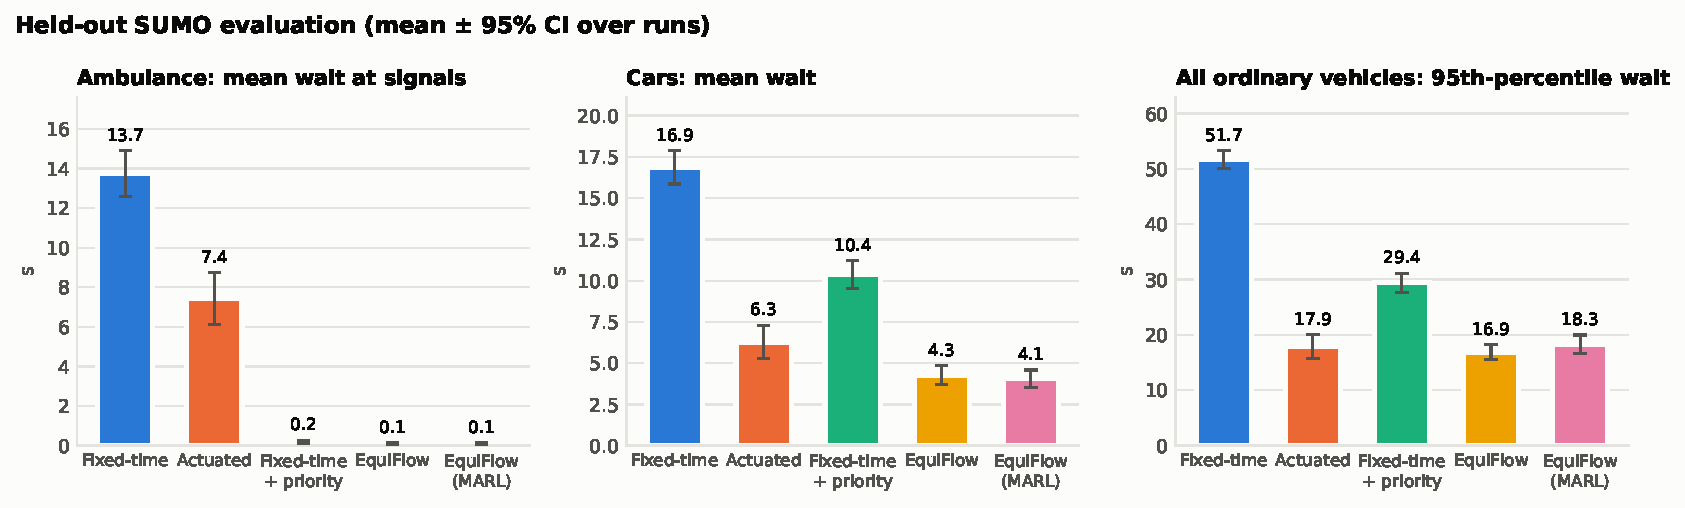
\includegraphics[width=\textwidth]{figures/fig_main_comparison.pdf}
\caption{Held-out evaluation: ambulance wait, car wait and 95th-percentile wait per controller
(mean $\pm$ 95\% CI over 120 runs each).}
\label{fig:it2-main}
\end{figure}

Table~\ref{tab:it2-main} and Figure~\ref{fig:it2-main} give the main comparison. EquiFlow reduces the
ambulance's mean wait at signals from 13.75\,s (fixed-time) and 7.42\,s (actuated) to 0.10\,s, and its travel
time by 16.5\,s (28\%) and 10.1\,s (19\%) respectively. Ordinary traffic also waits less: car wait is 4.28\,s
against 16.87\,s for fixed-time and 6.28\,s for actuated. The paired comparison (Table~\ref{tab:it2-paired})
puts the advantage over actuated at $-2.00 \pm 0.61$\,s (better in 68\% of paired runs), and the worst-served
approach waits 2.3\,s less. The 95th-percentile wait ($-0.96 \pm 1.32$\,s), the longest single wait
($+3.1 \pm 3.3$\,s) and the Jain index across approaches are statistically level with actuated. The price of
priority is paid by the vehicles an ambulance holds: they wait 19.6\,s on average, against 12.4\,s with actuated
control (which never holds them), 25.2\,s with fixed-time plus simple priority and 36.2\,s with fixed-time.

\begin{figure}[htbp]
\centering
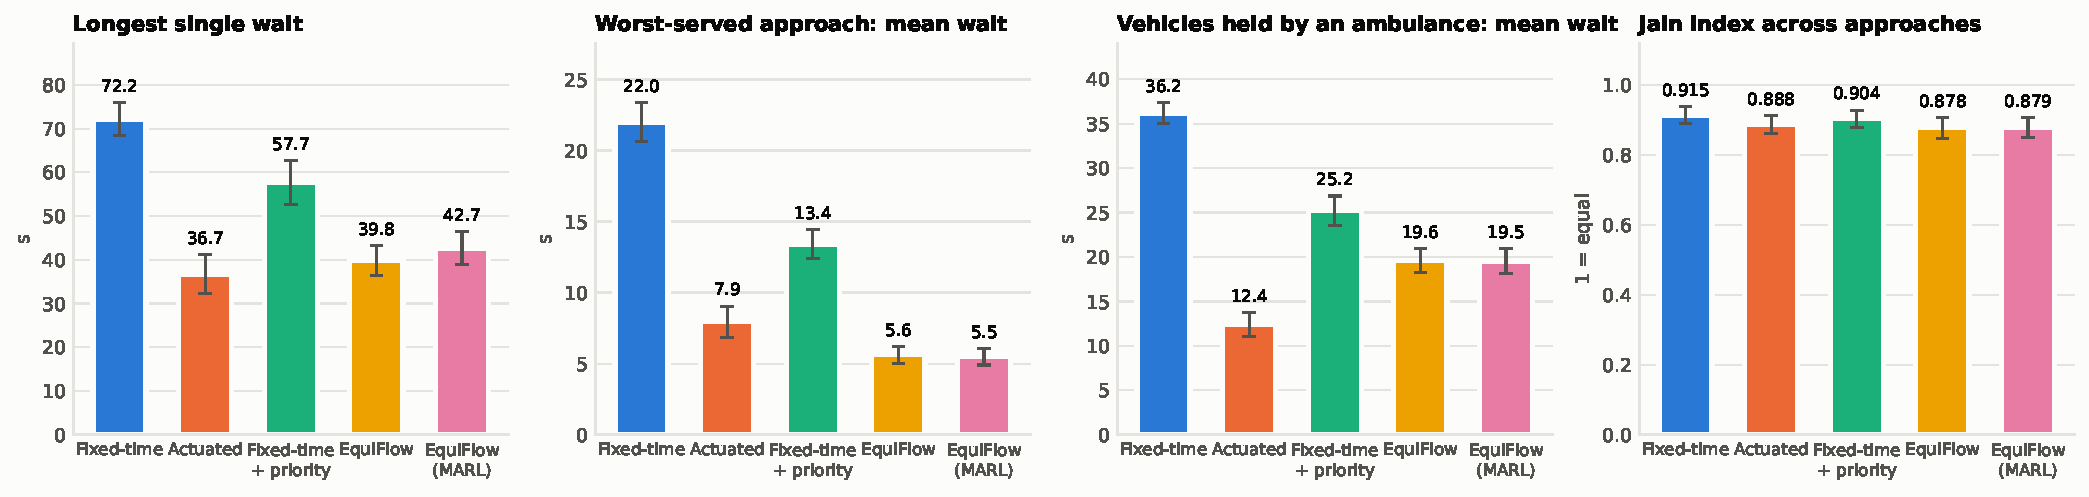
\includegraphics[width=\textwidth]{figures/fig_fairness.pdf}
\caption{Fairness: longest single wait, the worst-served approach's mean wait, the mean wait of the vehicles
held by an ambulance, and Jain's index across approaches.}
\label{fig:it2-fairness}
\end{figure}

\begin{figure}[htbp]
\centering
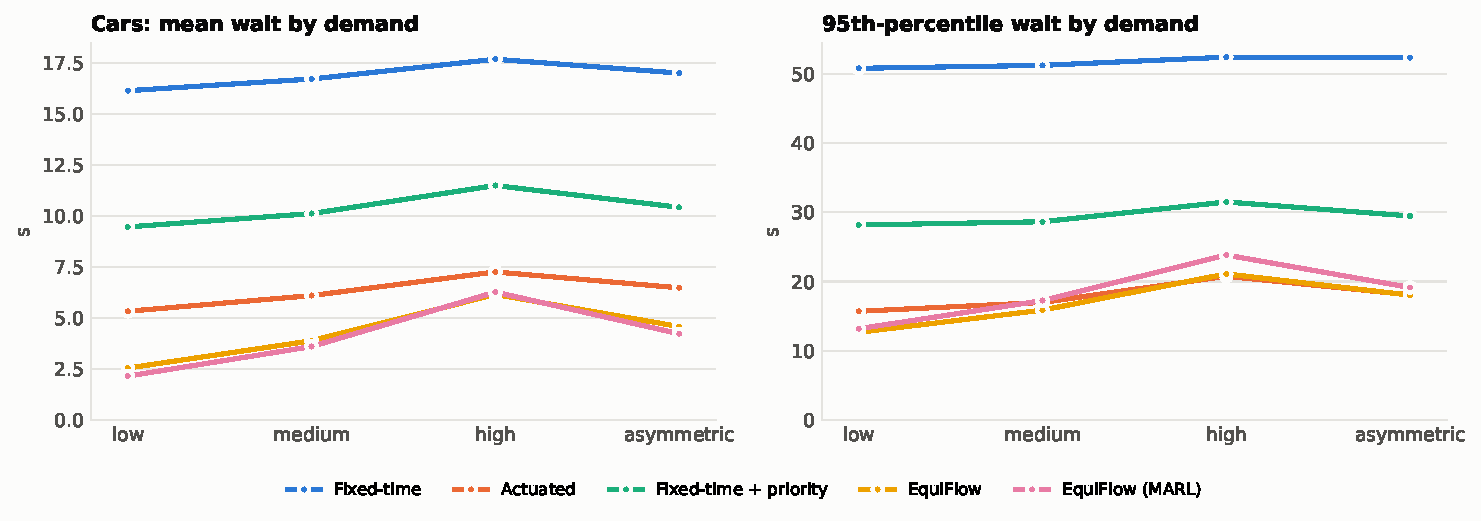
\includegraphics[width=\textwidth]{figures/fig_by_demand.pdf}
\caption{Car mean wait and 95th-percentile wait by demand level.}
\label{fig:it2-demand}
\end{figure}

Under heavy demand (Figure~\ref{fig:it2-demand}) EquiFlow's car wait is below actuated (6.15 against
7.25\,s; 6.92\,s in the first evaluation), and its 95th-percentile wait is now level (21.10 against 20.76\,s, a
paired difference of $+0.33 \pm 2.87$\,s, against $+1.68$\,s in the first evaluation). This is despite every
EquiFlow phase change costing 3\,s of yellow and 2\,s of all-red, against 4\,s of yellow and no all-red in SUMO's
actuated plans; the all-red is kept for safety.

\subsection{Ablations}
\label{sec:it2-ablation}
\begin{figure}[htbp]
\centering
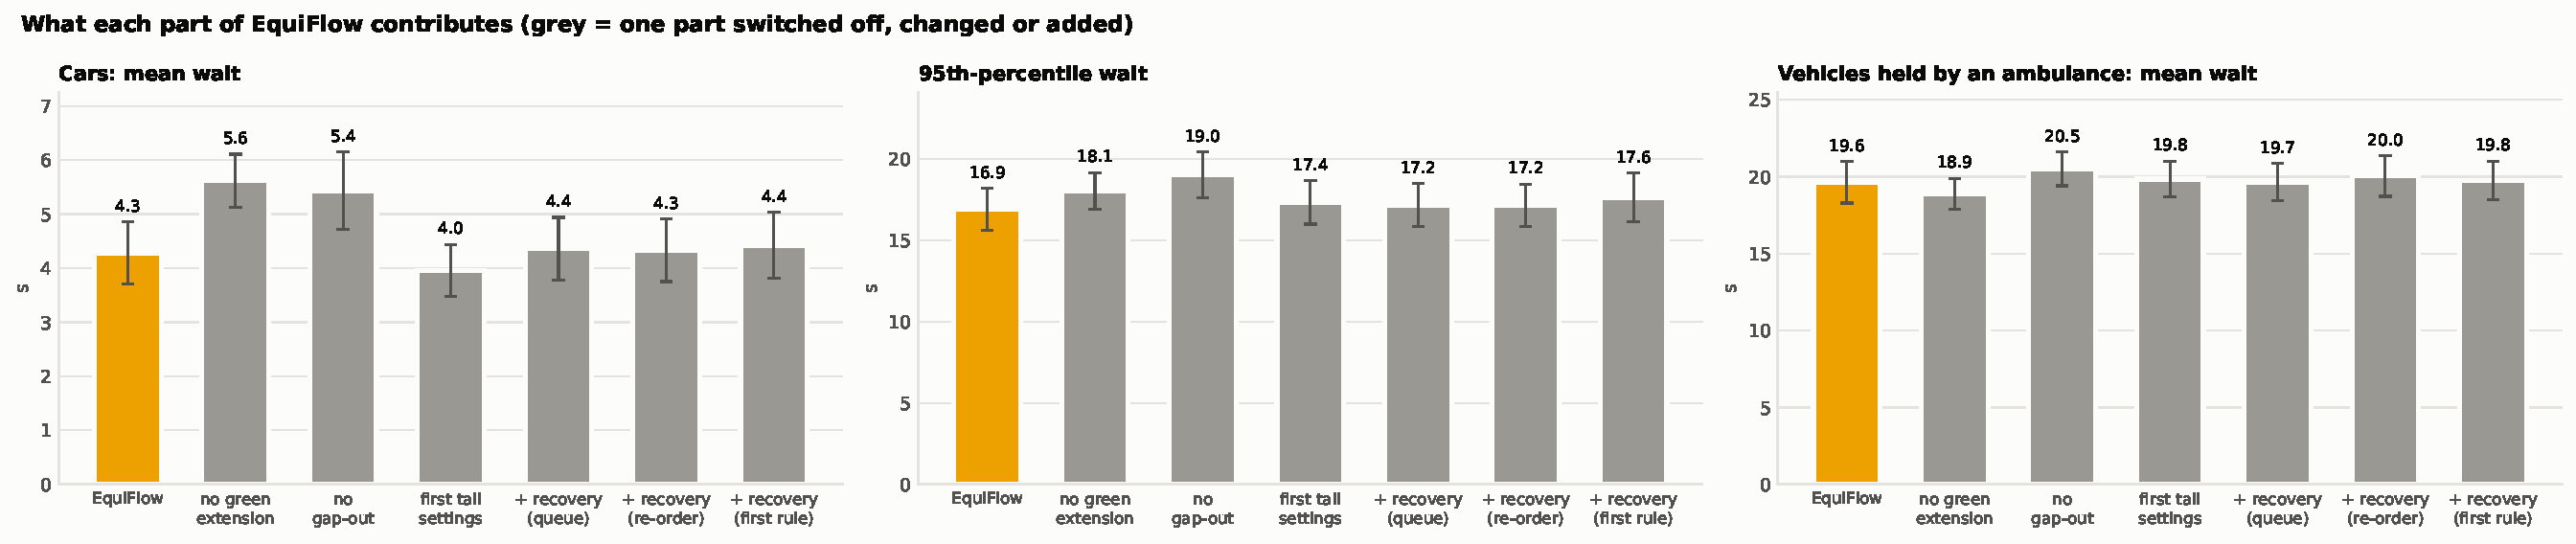
\includegraphics[width=\textwidth]{figures/fig_ablation.pdf}
\caption{Ablations: EquiFlow with one component switched off or replaced.}
\label{fig:it2-ablation}
\end{figure}

Table~\ref{tab:it2-ablation} and Figure~\ref{fig:it2-ablation} switch one component off, change it, or add an
optional one back. \emph{Green extension} gives the largest gain in average waits: without it car wait rises by
1.33\,s (better with it in 95\% of paired runs) and the 95th-percentile wait by 1.16\,s, with no significant
change in the longest wait. In the first evaluation round extension cost 6.6\,s on the longest wait; the tighter
30\,s wait cap and the higher waiting-time weight removed that cost (the first settings have a 4.4\,s longer
longest wait), at 0.3\,s of car wait. \emph{Gap-out} improves every measure: without it car wait rises by 1.15\,s
and the 95th-percentile wait by 2.11\,s (better in 99\% of runs).

\emph{Fair recovery} gives no benefit with any of the three rules. Adding the queue-sized rule raises car wait
by 0.08\,s and the 95th-percentile wait by 0.26\,s; the re-order-only rule changes nothing significantly except a
0.25\,s higher 95th-percentile wait; the first rule is worst (95th percentile +0.74\,s, longest wait +2.2\,s). The
stress scenario (about 40 ambulances per hour, 30 runs per controller) gives the same answer: the queue-sized rule
raises the 95th-percentile wait by 1.3\,s, the first rule by 4.0\,s, and the re-order rule by nothing measurable.
Re-ordering removes the harm but adds no benefit: an adaptive controller that already serves the
longest-waiting busy approach next leaves nothing for a separate recovery phase to fix. Recovery is therefore off
by default.

On the two multi-junction networks (Table~\ref{tab:it2-corridor}) the \emph{green corridor} turns downstream
signals green a little earlier but does not change ambulance travel time, while the vehicles it holds wait
longer: 2.4\,s with the just-in-time rule and 6.8\,s with the first rule. With junctions 300\,m apart, local
priority alone is fast enough, so the corridor is off by default.

\subsection{MARL controller}
\begin{figure}[htbp]
\centering
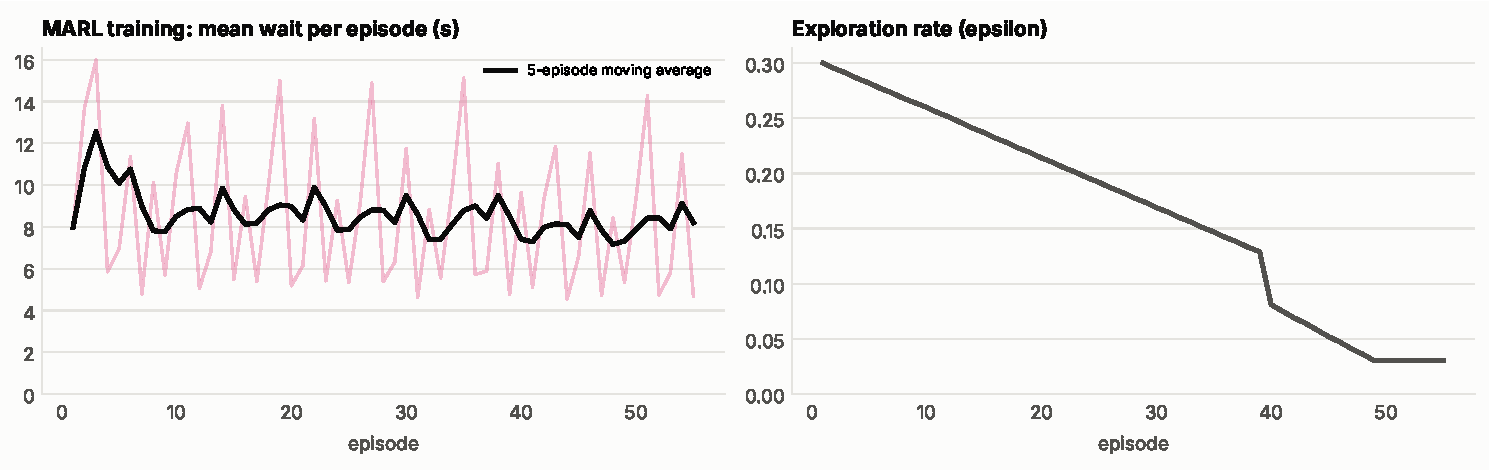
\includegraphics[width=\textwidth]{figures/fig_marl_training.pdf}
\caption{MARL training: mean wait per episode (episodes rotate between networks) and exploration rate.}
\label{fig:it2-marl}
\end{figure}

The first MARL policy (55 training episodes) tied the adaptive heuristic on car wait but had a 1.85\,s higher
95th-percentile wait. Its reward was therefore extended to charge every halted vehicle that has already waited
more than 20\,s (about the 95th-percentile wait), and it was retrained from scratch for 120 episodes on seeds
1--5 with the final junction settings. On the held-out seeds it now beats the heuristic on car wait
($-0.23 \pm 0.18$\,s), but the heuristic's own tail tuning moved further, so MARL's 95th-percentile wait is
$1.43 \pm 0.55$\,s higher and its longest wait 2.9\,s higher, with the same picture on network/demand combinations
it was trained on and on unseen ones (Table~\ref{tab:it2-marl}). The adaptive controller stays the default.

\subsection{Robustness to camera errors}
\begin{figure}[htbp]
\centering
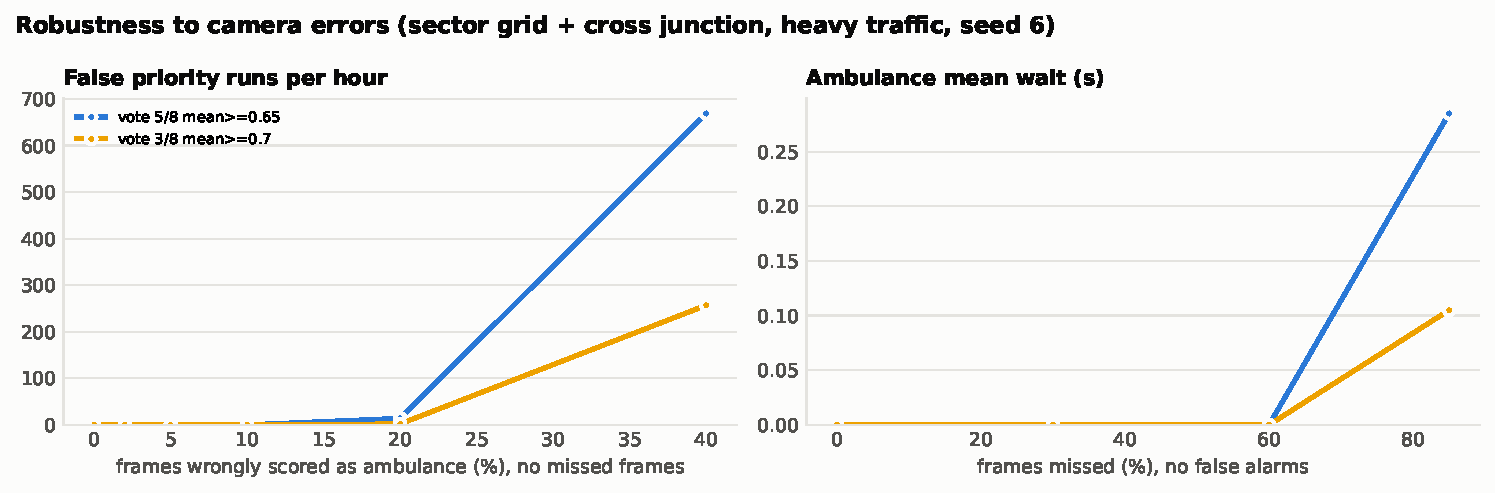
\includegraphics[width=\textwidth]{figures/fig_robustness.pdf}
\caption{False priority runs and ambulance wait as the virtual camera misses frames or scores ordinary
vehicles as ambulances, for the 5-of-8 vote and the live 3-of-8 vote (heavy demand, seed 6).}
\label{fig:it2-robust}
\end{figure}

The sweep was run for both votes (Figure~\ref{fig:it2-robust}). With up to 10\% of frames wrongly scored as
ambulance, neither produces any false priority. At 20\% the 5-of-8 vote (mean $\geq$ 0.65) produces 8--20 false
priority runs per hour and the live 3-of-8 vote (mean $\geq$ 0.70) only 0--4; at 40\% they produce 386--952
and 145--369. The live vote is therefore more tolerant of noisy frames, not less: its stricter mean-score
threshold matters more than the lower vote count. Missing even 85\% of frames barely matters (ambulance wait at
most 0.6\,s). The classifier's per-crop false-alarm rate is 0.9\% on the test split, well inside this margin.

\subsection{Ambulance classifier}
\label{sec:it2-classifier}
\paragraph{Dataset check.} \texttt{Projects/make\_split\_manifest.py} lists all 32\,593 crops with a SHA-1 and a
perceptual hash and looks for images shared between splits. The test split contains no exact copy of a training
image; 134 test crops (3.6\%) are near duplicates of a training crop, all with the same label. The check found
four validation crops labelled ambulance that were copies of training crops labelled other vehicle, and 35
duplicate files inside the training split; all 39 were removed. Removing the four mislabelled copies alone raised
the mid-report model's validation recall from 91.0\% to 91.8\%: all four had been counted as missed ambulances.

\paragraph{Retraining.} Three changes proposed in the mid-report were trained one at a time on the cleaned data and
compared on the validation split only (Table~\ref{tab:it2-cls-val}). Retraining with unchanged settings changes
little; doubling the ambulance crops gives the highest recall but more false alarms; a 128\,px input
(cls\_v5\_img128) is best on PR-AUC and F1 and was selected.

\paragraph{Test split.} Only the selected model and the mid-report model were then run on the held-out test split,
once (Table~\ref{tab:it2-cls-test}). cls\_v5\_img128 is better on every metric: 93.5\% recall at 96.5\% precision
and a 0.9\% false-alarm rate. Recall is lowest on the Pakistani ambulance crops (88.1\%, against 95.9\% on the
public dataset). A threshold chosen on the validation split for 95\% recall gives 95.7\% test recall for the
mid-report model, at 87.7\% precision.

\paragraph{Latency.} On an RTX 4050 laptop GPU the vehicle detector takes 27.7\,ms per 1280\,px frame and the
classifier 1.7\,ms per crop in a batch (Table~\ref{tab:it2-latency}): about 45\,ms per frame, or 22 frames per
second, with ten vehicles in view. Measured back to back, the 128\,px classifier costs the same as the 96\,px one.

\subsection{Tracking on real video}
\label{sec:it2-tracking}
With the new classifier and the old vote (5 of 8, mean $\geq$ 0.65) the pipeline confirmed 5 of the 7 labelled
ambulance passes. \texttt{Projects/tune\_tracking.py} records every track's score per frame once and replays the
vote offline; at the old setting the replay reproduces the pipeline's confirmations exactly on all 12 videos.
Of 360 settings (Table~\ref{tab:it2-tune}), the number of votes K decides the result: every setting with K = 3
and a mean score of 0.70--0.75 confirms all 7 passes with 6 false events, whatever the frame threshold, while
K = 4 or 5 confirm 5. The chosen setting keeps the frame threshold at 0.6 and uses K = 3, mean $\geq$ 0.70.

Table~\ref{tab:it2-tracking} gives the re-run pipeline on all 12 available clips (a thirteenth clip has no source
video): 7 of 7 passes confirmed, on average 0.94\,s after the labelled start, with 6 false confirmations: 3 in
test5, a clip checked to contain no ambulance (a look-alike vehicle), 2 in test12 1.4\,s before a labelled pass,
and 1 in test4. Because the same videos chose and scored the setting, this is optimistic. Choosing the setting on
11 videos and scoring the twelfth, for each video in turn, gives 7 of 7 passes and 11 false events. Seven passes
are far too few for a reliable recall estimate.

\subsection{Performance}
A controller tick takes about 1\,$\mu$s and a MARL decision about 24\,$\mu$s (p99 62\,$\mu$s), against a
100\,000\,$\mu$s tick period (Table~\ref{tab:it2-perf}). A one-hour SUMO run takes about 3\,s.

\section{Failure Analysis}
\begin{table}[htbp]
\centering
\small
\caption{Failure cases found in Iteration 2 and the planned response.}
\label{tab:it2-failures}
\resizebox{\textwidth}{!}{%
\begin{tabular}{lll}
\hline
Failure & Likely cause & Response \\
\hline
Short ambulance tracks missed with a 5-of-8 vote (test12) & too few confident frames before it leaves & resolved: K = 3, re-tuned \\
3 false confirmations in test5 (no ambulance) & ambulance-like vehicle not in training & add its crops as hard negatives \\
Early confirmations (test12, 1.4\,s before the label) & hand-labelled windows are approximate & label from the first visible frame \\
Recall 88\% on Pakistani ambulances (test) & few local ambulance crops in training & collect more local ambulance crops \\
Mislabelled duplicate crops (4 in validation) & copies made while sorting crops & resolved: split manifest + duplicate check \\
False priority at $\geq$20\% per-frame false alarms & vote too permissive for very noisy input & keep per-frame FP $\ll$ 20\%; live 3-of-8 vote is 4$\times$ more tolerant \\
Higher p95 wait than actuated under heavy demand & green length fixed at its start & resolved: extension + tail tuning (gap +0.3\,s, n.s.) \\
Green extension lengthened the longest wait (+6.6\,s) & others held up to the 40\,s cap & resolved: 30\,s cap, wait weight 0.3 \\
Corridor gives no measurable ambulance benefit & junctions 300\,m apart & off by default; just-in-time rule kept as an option \\
Fair recovery gives no benefit (harmful when frequent) & adaptive order already serves delayed approaches & off by default; re-order rule removes the harm \\
MARL better on car wait, worse on tail waits & heuristic tail tuning moved further & longer training, tail-weighted reward \\
\hline
\end{tabular}}
\end{table}

\section{Limitations}
All control results are from simulation; the SUMO cameras are virtual (exact ambulance positions with
simulated classifier scores), so the real camera pipeline and the SUMO evaluation share the controller and the
voting rule but not the video. The live vote (3 of 8) was tuned on the same 12 clips it is scored on, which
hold only 7 ambulance passes. The fair-recovery stress scenario is one synthetic demand pattern. Authentication
is off by default and must be enabled for any deployment.

\section{Iteration Outcome}
The exit criterion is met: the scripted scenario (\texttt{scripts/scripted\_scenario.py}) sends one ambulance,
then two simultaneous ambulances; each is confirmed by detection, receives a protected green, and is followed
by recovery greens, and the whole sequence is recorded in the event log. All 45 automated tests pass. The classifier
was evaluated on the held-out test split and replaced by a better retrained model, all available videos were
processed, and the improvements the first evaluation pointed to were implemented and evaluated on the held-out
seeds: green extension and tail tuning (which closed the heavy-demand gap to actuated control), an approach-level
fairness measure, a re-order-only recovery rule and a recovery stress test, a just-in-time corridor, a retrained
MARL policy and the camera-error sweep for the live vote. Fair recovery and the corridor did not help and are off
by default. The main open items for FYP-2 are reducing the delay of the vehicles an ambulance holds (the cost of
priority that remains), MARL training that also wins on tail waits, more labelled real video, and hard negatives
for ambulance look-alikes.
 after chapter6_iteration1.
% Needs \usepackage{graphicx} (loaded by most report classes).
% All numbers come from sumo/results/heldout/*.csv and the Projects/ evaluation outputs (see docs/RESULTS.md);
% the tables are generated by sumo/latex_tables.py and should be regenerated rather than edited.

\chapter{Iteration 2: Tracking, Control, Integration and Evaluation}
\label{ch:iteration2}

\section{Iteration Objectives}
Iteration~2 turns the perception and simulation work of Iteration~1 into a working, measured system.
Its objectives, taken from the iteration plan, were to:
(i) track ambulances across frames so that a single confident frame cannot trigger priority;
(ii) give a confirmed ambulance a protected green through safe yellow and all-red transitions, also across
neighbouring junctions (green corridor);
(iii) restore service to delayed approaches afterwards (fair recovery) and add a fairness-aware MARL base
controller;
(iv) integrate the modules behind FastAPI and MQTT with a live dashboard; and
(v) evaluate the controllers on repeatable SUMO runs against fixed-time and actuated baselines.
The exit criterion was that a scripted ambulance scenario triggers and completes a logged preemption with
recovery.

\section{Selected Use Cases / Features}
UC-01 (detect an approaching ambulance), UC-02 (estimate traffic state), UC-03 (grant emergency priority),
UC-04 (recover fairly after priority), UC-05 (run a baseline comparison) and UC-06 (monitor the junction on
the dashboard). Requirement coverage after this iteration is summarised in Table~\ref{tab:it2-req}.

\begin{table}[htbp]
\centering
\small
\caption{Functional requirements and test cases addressed in Iteration 2.}
\label{tab:it2-req}
\resizebox{\textwidth}{!}{%
\begin{tabular}{lll}
\hline
Requirement / test & Implementation & Evidence \\
\hline
FR-01--03 detection input, output, logging & \texttt{vision/live.py}, \texttt{eventlog.py} & \texttt{test\_live\_pipeline.py}, CSV event log \\
FR-04 traffic state & SUMO queues; camera approach zones (\texttt{zones:}) & \texttt{test\_fr04\_zone\_...} \\
FR-05 / TC-03 stale detections & 2\,s age limit on external events, K-of-M vote, 60\,s fail-safe & \texttt{test\_tc03\_...} \\
FR-06--08 phases, timing, priority & \texttt{controllers/intersection.py} & \texttt{test\_controller.py} (randomised safety) \\
FR-07 / TC-04 early end of empty green & gap-out after 5\,s, only if another approach has demand & \texttt{test\_tc04\_...} \\
FR-09 / TC-06 logged preemption and recovery & event log + episode table & \texttt{scripts/scripted\_scenario.py} \\
FR-10 recovery uses queue and wait & queue-sized recovery greens, longest wait first & \texttt{test\_fr10\_...} \\
FR-11 baselines & fixed-time, actuated, fixed-time + priority & Section~\ref{sec:it2-results} \\
FR-12 export metrics and configuration & \texttt{run\_manifest.csv} (config + versions per run) & \texttt{results/heldout/} \\
TC-10 repeatability & same seed and configuration give identical results & \texttt{test\_tc10\_...} \\
\hline
\end{tabular}}
\end{table}

\section{Design}
The controller is split into a \emph{base controller} that chooses the next green in normal operation
(fixed-time, adaptive, or the MARL policy) and an \emph{intersection controller} that wraps it with
everything that must never be learned: ambulance priority, minimum green, yellow and all-red, the 90\,s
maximum-wait guard, gap-out and fair recovery. The intersection controller never reads a clock; it is
given the time on every tick, so the same code runs in the live backend (every 0.1\,s) and inside each SUMO
step. Every decision is published as an event on a bus that feeds the REST/WebSocket API, the optional MQTT
bridge and a CSV event log.

\section{Implementation}
\begin{itemize}
\item \textbf{Perception} (\texttt{backend/app/vision/live.py}): YOLO26s vehicle detection with ByteTrack,
the ambulance classifier on each tracked crop (cls\_v5\_img128, retrained in this iteration at 128\,px), and a
confirmation vote over the last 8 frames. The live camera configuration needs 3 ambulance votes (frame score
$\geq$ 0.6) and a mean score of at least 0.70, re-tuned for the new classifier
(Section~\ref{sec:it2-tracking}); the SUMO evaluation and the backend default use 5 of 8 with mean
$\geq$ 0.65. Optional per-approach polygons restrict counting to the lanes that queue for the signal and
report stationary vehicles as the queue.
\item \textbf{Signal control} (\texttt{backend/app/controllers/}): base controllers, the MARL policy
(shared Q-network over per-phase features, pure NumPy) and the intersection controller described above.
\item \textbf{Integration} (\texttt{backend/app/}): FastAPI REST + WebSocket + MJPEG, MQTT topics, a live
SUMO view driven through TraCI, an optional API key on every write endpoint, and the CSV event log.
\item \textbf{Evaluation} (\texttt{sumo/}): \texttt{run\_matrix.py} runs every controller on the same
networks, demand levels and seeds in parallel; \texttt{aggregate.py} computes means, confidence intervals and
paired differences; \texttt{make\_plots.py} and \texttt{latex\_tables.py} produce the figures and tables in
this chapter.
\end{itemize}

\section{Algorithms and Technical Decisions}
\paragraph{Gap-out.} A green that has run at least 5\,s ends early when no vehicle is within 120\,m of its
stop line and another approach has demand. It is never applied during priority and always passes through
the full yellow and all-red.
\paragraph{Green extension.} Actuated control lengthens a green vehicle by vehicle, while the adaptive controller
fixes each green's length when it starts. A base-controller green that reaches its planned length therefore keeps
going while its approach is still at least as busy as every other one, up to 45\,s, and only while no other
approach with a queue has waited 30\,s. To keep the tail of the waiting-time distribution short, the adaptive
controller also weights waiting time more when it chooses the next green (weight 0.3 instead of 0.1). It is never applied during priority or recovery, and every green still
ends through the full yellow and all-red. The two limits were chosen on tuning seeds 1--2, not on the held-out
seeds.
\paragraph{Priority.} After the vote confirms an ambulance, the current green finishes its minimum time,
then yellow and all-red, and the ambulance's approach turns green alone. Priority ends 4\,s after the
ambulance was last seen, or after 60\,s as a fail-safe. Two ambulances are served first come, first served.
\paragraph{Fair recovery.} After priority, the approaches that were held red and have a queue are served in
order of longest wait, each for about as long as its queue needs to clear (2\,s per queued vehicle, at least
5\,s, at most 30\,s). A first version gave every delayed approach a fixed 15\,s green plus extra, and a third
rule only re-orders the delayed approaches and leaves each green's length to the base controller. Because none of
them improved on having no recovery (Section~\ref{sec:it2-ablation}), recovery is off by default and kept as an
option; the scripted exit scenario switches it on to verify the logged recovery sequence.
\paragraph{Green corridor.} Once a camera confirms an ambulance, signals further along its route are asked for
priority \emph{just in time}: only when the ambulance's arrival time is within the time that signal needs to
switch to it (minimum green, yellow and all-red) plus 3\,s, or, if its phase is already green, when that green
would otherwise end just before the ambulance arrives. The first version cleared every signal within 25\,s of
arrival. Neither made ambulances faster on the evaluated networks, so the corridor is off by default.
\paragraph{Stale detections.} An externally reported detection older than 2\,s (or more than 2\,s in the
future) is rejected and logged, so a delayed or replayed message cannot request priority.

\section{Evaluation Set-up}
Six signalised Islamabad junction networks were each run at four demand levels for one simulated hour.
Every controller used the same 120 network/demand/seed combinations with seeds 6--10; the MARL policy was
trained on seeds 1--5, so all evaluation runs are held out. Ambulances are confirmed by a virtual camera per
approach using the real voting rule. Results are reported as mean $\pm$ 95\% confidence interval over runs,
and as \emph{paired} differences on identical runs, which removes the large differences between networks.
Besides network-wide waits, an approach-level measure counts the vehicles an ambulance actually holds: ordinary
vehicles stopped at a junction while a real ambulance is within camera range on another of its approaches. It is
ground truth, so it is measured the same way for controllers that give no priority. A stress scenario (heavy
traffic and about 40 ambulances per hour, three times the heavy level) tests fair recovery separately.

% Generated by sumo/latex_tables.py from the CSV results. Do not edit by hand; re-run the script.

\begin{table}[htbp]
\centering
\small
\caption{Held-out evaluation: mean $\pm$ 95\% confidence interval over one-hour SUMO runs (seeds 6--10).}
\label{tab:it2-main}
\resizebox{\textwidth}{!}{%
\begin{tabular}{lccccc}
\hline
Metric & Fixed-time & Actuated & Fixed + priority & EquiFlow & EquiFlow (MARL) \\
\hline
Car mean wait (s) & 16.87 $\pm$ 1.02 & 6.28 $\pm$ 1.01 & 10.36 $\pm$ 0.86 & 4.28 $\pm$ 0.57 & 4.05 $\pm$ 0.53 \\
Ordinary vehicles, mean wait (s) & 17.07 $\pm$ 1.05 & 6.23 $\pm$ 0.99 & 10.29 $\pm$ 0.84 & 4.32 $\pm$ 0.56 & 4.10 $\pm$ 0.52 \\
95th-percentile wait (s) & 51.71 $\pm$ 1.61 & 17.87 $\pm$ 2.13 & 29.44 $\pm$ 1.69 & 16.91 $\pm$ 1.31 & 18.34 $\pm$ 1.65 \\
Longest single wait (s) & 72.17 $\pm$ 3.72 & 36.71 $\pm$ 4.45 & 57.69 $\pm$ 5.03 & 39.84 $\pm$ 3.34 & 42.69 $\pm$ 3.72 \\
Share waiting $>$60 s & 0.030 $\pm$ 0.005 & 0.002 $\pm$ 0.001 & 0.002 $\pm$ 0.001 & 0.001 $\pm$ 0.000 & 0.001 $\pm$ 0.001 \\
Worst approach, mean wait (s) & 21.98 $\pm$ 1.37 & 7.95 $\pm$ 1.10 & 13.40 $\pm$ 1.01 & 5.63 $\pm$ 0.59 & 5.49 $\pm$ 0.58 \\
Jain index across approaches & 0.915 $\pm$ 0.025 & 0.888 $\pm$ 0.025 & 0.904 $\pm$ 0.025 & 0.878 $\pm$ 0.030 & 0.879 $\pm$ 0.029 \\
Held by an ambulance, mean wait (s) & 36.17 $\pm$ 1.16 & 12.39 $\pm$ 1.37 & 25.22 $\pm$ 1.63 & 19.64 $\pm$ 1.35 & 19.55 $\pm$ 1.43 \\
Held by an ambulance, p95 wait (s) & 56.02 $\pm$ 2.19 & 22.53 $\pm$ 3.00 & 39.74 $\pm$ 3.26 & 29.47 $\pm$ 2.18 & 31.80 $\pm$ 3.17 \\
Ambulance mean wait (s) & 13.75 $\pm$ 1.16 & 7.42 $\pm$ 1.31 & 0.19 $\pm$ 0.08 & 0.10 $\pm$ 0.06 & 0.10 $\pm$ 0.05 \\
Ambulance travel time (s) & 59.14 $\pm$ 2.42 & 52.75 $\pm$ 2.40 & 43.19 $\pm$ 2.21 & 42.68 $\pm$ 2.22 & 42.54 $\pm$ 2.22 \\
Detection to green (s) & -- & -- & 2.57 $\pm$ 0.17 & 2.37 $\pm$ 0.13 & 2.39 $\pm$ 0.16 \\
Recovery interval (s) & -- & -- & 0.00 $\pm$ 0.00 & 0.00 $\pm$ 0.00 & 0.00 $\pm$ 0.00 \\
Runs & 120 & 120 & 120 & 120 & 120 \\
\hline
\end{tabular}}
\end{table}

\begin{table}[htbp]
\centering
\small
\caption{Ablations: EquiFlow with one component switched off, changed or added (all networks).}
\label{tab:it2-ablation}
\resizebox{\textwidth}{!}{%
\begin{tabular}{lccccccc}
\hline
Metric & EquiFlow & No extension & No gap-out & First tail settings & + Recovery (queue) & + Recovery (re-order) & + Recovery (first rule) \\
\hline
Car mean wait (s) & 4.28 $\pm$ 0.57 & 5.62 $\pm$ 0.49 & 5.43 $\pm$ 0.71 & 3.96 $\pm$ 0.48 & 4.36 $\pm$ 0.58 & 4.33 $\pm$ 0.58 & 4.42 $\pm$ 0.61 \\
95th-percentile wait (s) & 16.91 $\pm$ 1.31 & 18.07 $\pm$ 1.12 & 19.02 $\pm$ 1.41 & 17.35 $\pm$ 1.34 & 17.17 $\pm$ 1.32 & 17.16 $\pm$ 1.31 & 17.65 $\pm$ 1.49 \\
Longest single wait (s) & 39.84 $\pm$ 3.34 & 38.48 $\pm$ 3.82 & 42.21 $\pm$ 3.22 & 44.19 $\pm$ 3.08 & 39.78 $\pm$ 3.32 & 40.31 $\pm$ 3.60 & 41.99 $\pm$ 3.90 \\
Jain index across approaches & 0.878 $\pm$ 0.030 & 0.911 $\pm$ 0.025 & 0.889 $\pm$ 0.029 & 0.864 $\pm$ 0.032 & 0.881 $\pm$ 0.030 & 0.880 $\pm$ 0.030 & 0.877 $\pm$ 0.030 \\
Held by an ambulance, mean wait (s) & 19.64 $\pm$ 1.35 & 18.89 $\pm$ 1.00 & 20.50 $\pm$ 1.09 & 19.84 $\pm$ 1.17 & 19.66 $\pm$ 1.21 & 20.04 $\pm$ 1.32 & 19.77 $\pm$ 1.24 \\
Ambulance mean wait (s) & 0.10 $\pm$ 0.06 & 0.13 $\pm$ 0.06 & 0.14 $\pm$ 0.08 & 0.10 $\pm$ 0.04 & 0.10 $\pm$ 0.05 & 0.10 $\pm$ 0.06 & 0.08 $\pm$ 0.03 \\
Ambulance travel time (s) & 42.68 $\pm$ 2.22 & 42.92 $\pm$ 2.22 & 42.82 $\pm$ 2.22 & 42.57 $\pm$ 2.22 & 42.65 $\pm$ 2.22 & 42.66 $\pm$ 2.22 & 42.63 $\pm$ 2.21 \\
Recovery interval (s) & 0.00 $\pm$ 0.00 & 0.00 $\pm$ 0.00 & 0.00 $\pm$ 0.00 & 0.00 $\pm$ 0.00 & 22.94 $\pm$ 0.94 & 21.61 $\pm$ 0.88 & 28.25 $\pm$ 1.35 \\
Runs & 120 & 120 & 120 & 120 & 120 & 120 & 120 \\
\hline
\end{tabular}}
\end{table}

\begin{table}[htbp]
\centering
\small
\caption{Green corridor on the two multi-junction networks (sector grid, diamond): EquiFlow (no corridor) minus EquiFlow with each corridor rule, on identical runs. Negative = EquiFlow lower. $^*$: the 95\% CI excludes zero.}
\label{tab:it2-corridor}
\begin{tabular}{llccc}
\hline
Versus & Metric & Difference (95\% CI) & EquiFlow better in & Runs \\
\hline
+ Corridor (just in time) & Car mean wait (s) & -0.06 $\pm$ 0.07 & 40\% & 40 \\
+ Corridor (just in time) & 95th-percentile wait (s) & -0.37 $\pm$ 0.32$^*$ & 32\% & 40 \\
+ Corridor (just in time) & Longest single wait (s) & -0.17 $\pm$ 1.30 & 22\% & 40 \\
+ Corridor (just in time) & Held by an ambulance, mean wait (s) & -2.43 $\pm$ 1.31$^*$ & 63\% & 35 \\
+ Corridor (just in time) & Ambulance mean wait (s) & -0.02 $\pm$ 0.03 & 8\% & 40 \\
+ Corridor (just in time) & Ambulance travel time (s) & +0.04 $\pm$ 0.12 & 18\% & 40 \\
+ Corridor (25 s ETA) & Car mean wait (s) & -0.06 $\pm$ 0.07 & 55\% & 40 \\
+ Corridor (25 s ETA) & 95th-percentile wait (s) & -0.71 $\pm$ 0.47$^*$ & 52\% & 40 \\
+ Corridor (25 s ETA) & Longest single wait (s) & -4.33 $\pm$ 2.17$^*$ & 60\% & 40 \\
+ Corridor (25 s ETA) & Held by an ambulance, mean wait (s) & -6.76 $\pm$ 1.92$^*$ & 91\% & 35 \\
+ Corridor (25 s ETA) & Ambulance mean wait (s) & -0.01 $\pm$ 0.02 & 2\% & 40 \\
+ Corridor (25 s ETA) & Ambulance travel time (s) & +0.08 $\pm$ 0.11 & 20\% & 40 \\
\hline
\end{tabular}
\end{table}

\begin{table}[htbp]
\centering
\small
\caption{Paired comparison on identical runs (same network, demand and seed): EquiFlow minus the other controller. Negative values mean EquiFlow is lower. $^*$: the 95\% CI excludes zero.}
\label{tab:it2-paired}
\begin{tabular}{llccc}
\hline
Versus & Metric & Difference (95\% CI) & EquiFlow better in & Runs \\
\hline
Fixed-time & Car mean wait (s) & -12.59 $\pm$ 0.66$^*$ & 100\% & 120 \\
Fixed-time & 95th-percentile wait (s) & -34.80 $\pm$ 1.19$^*$ & 100\% & 120 \\
Fixed-time & Longest single wait (s) & -32.33 $\pm$ 3.77$^*$ & 97\% & 120 \\
Fixed-time & Ambulance mean wait (s) & -13.64 $\pm$ 1.13$^*$ & 100\% & 120 \\
Actuated & Car mean wait (s) & -2.00 $\pm$ 0.61$^*$ & 68\% & 120 \\
Actuated & 95th-percentile wait (s) & -0.96 $\pm$ 1.32 & 48\% & 120 \\
Actuated & Longest single wait (s) & +3.13 $\pm$ 3.28 & 30\% & 120 \\
Actuated & Ambulance mean wait (s) & -7.32 $\pm$ 1.29$^*$ & 99\% & 120 \\
Fixed + priority & Car mean wait (s) & -6.08 $\pm$ 0.42$^*$ & 100\% & 120 \\
Fixed + priority & 95th-percentile wait (s) & -12.53 $\pm$ 0.82$^*$ & 100\% & 120 \\
Fixed + priority & Longest single wait (s) & -17.85 $\pm$ 3.19$^*$ & 85\% & 120 \\
Fixed + priority & Ambulance mean wait (s) & -0.09 $\pm$ 0.06$^*$ & 28\% & 120 \\
EquiFlow (MARL) & Car mean wait (s) & +0.23 $\pm$ 0.18$^*$ & 48\% & 120 \\
EquiFlow (MARL) & 95th-percentile wait (s) & -1.43 $\pm$ 0.55$^*$ & 60\% & 120 \\
EquiFlow (MARL) & Longest single wait (s) & -2.85 $\pm$ 1.97$^*$ & 62\% & 120 \\
EquiFlow (MARL) & Ambulance mean wait (s) & +0.01 $\pm$ 0.05 & 12\% & 120 \\
No gap-out & Car mean wait (s) & -1.15 $\pm$ 0.18$^*$ & 99\% & 120 \\
No gap-out & 95th-percentile wait (s) & -2.11 $\pm$ 0.27$^*$ & 91\% & 120 \\
No gap-out & Longest single wait (s) & -2.37 $\pm$ 1.94$^*$ & 60\% & 120 \\
No gap-out & Ambulance mean wait (s) & -0.04 $\pm$ 0.05 & 17\% & 120 \\
No extension & Car mean wait (s) & -1.33 $\pm$ 0.18$^*$ & 95\% & 120 \\
No extension & 95th-percentile wait (s) & -1.16 $\pm$ 0.38$^*$ & 59\% & 120 \\
No extension & Longest single wait (s) & +1.36 $\pm$ 2.00 & 32\% & 120 \\
No extension & Ambulance mean wait (s) & -0.03 $\pm$ 0.04 & 21\% & 120 \\
First tail settings & Car mean wait (s) & +0.32 $\pm$ 0.13$^*$ & 34\% & 120 \\
First tail settings & 95th-percentile wait (s) & -0.44 $\pm$ 0.29$^*$ & 41\% & 120 \\
First tail settings & Longest single wait (s) & -4.35 $\pm$ 2.09$^*$ & 62\% & 120 \\
First tail settings & Ambulance mean wait (s) & +0.00 $\pm$ 0.05 & 11\% & 120 \\
+ Recovery (queue) & Car mean wait (s) & -0.08 $\pm$ 0.07$^*$ & 59\% & 120 \\
+ Recovery (queue) & 95th-percentile wait (s) & -0.26 $\pm$ 0.21$^*$ & 46\% & 120 \\
+ Recovery (queue) & Longest single wait (s) & +0.06 $\pm$ 1.72 & 42\% & 120 \\
+ Recovery (queue) & Ambulance mean wait (s) & +0.00 $\pm$ 0.03 & 9\% & 120 \\
+ Recovery (re-order) & Car mean wait (s) & -0.05 $\pm$ 0.06 & 53\% & 120 \\
+ Recovery (re-order) & 95th-percentile wait (s) & -0.25 $\pm$ 0.18$^*$ & 40\% & 120 \\
+ Recovery (re-order) & Longest single wait (s) & -0.47 $\pm$ 1.58 & 33\% & 120 \\
+ Recovery (re-order) & Ambulance mean wait (s) & +0.00 $\pm$ 0.04 & 3\% & 120 \\
+ Recovery (first rule) & Car mean wait (s) & -0.14 $\pm$ 0.09$^*$ & 59\% & 120 \\
+ Recovery (first rule) & 95th-percentile wait (s) & -0.74 $\pm$ 0.34$^*$ & 45\% & 120 \\
+ Recovery (first rule) & Longest single wait (s) & -2.15 $\pm$ 1.81$^*$ & 48\% & 120 \\
+ Recovery (first rule) & Ambulance mean wait (s) & +0.02 $\pm$ 0.05 & 8\% & 120 \\
\hline
\end{tabular}
\end{table}

\begin{table}[htbp]
\centering
\small
\caption{MARL minus adaptive EquiFlow on identical runs, split by whether the network/demand combination was used in MARL training. All seeds are unseen. Negative = MARL lower.}
\label{tab:it2-marl}
\begin{tabular}{lcc}
\hline
Metric & Trained combinations & Unseen combinations \\
\hline
Car mean wait (s) & -0.23 $\pm$ 0.27 (n=40) & -0.23 $\pm$ 0.24 (n=80) \\
95th-percentile wait (s) & +0.84 $\pm$ 0.54 (n=40) & +1.73 $\pm$ 0.77 (n=80) \\
Jain index across approaches & +0.001 $\pm$ 0.011 (n=40) & +0.001 $\pm$ 0.010 (n=80) \\
Ambulance mean wait (s) & +0.00 $\pm$ 0.03 (n=40) & -0.01 $\pm$ 0.07 (n=80) \\
\hline
\end{tabular}
\end{table}

\begin{table}[htbp]
\centering
\small
\caption{Signal controller timing on one CPU core (sumo/benchmark.py). The live backend ticks every 100\,000\,$\mu$s.}
\label{tab:it2-perf}
\begin{tabular}{lcccc}
\hline
Measured & Mean ($\mu$s) & Median & p99 & Max \\
\hline
tick (fixed\_time) & 0.94 & 0.92 & 3.21 & 99.37 \\
decision (fixed\_time) & 0.42 & 0.38 & 0.63 & 467.97 \\
tick (adaptive) & 1.07 & 0.95 & 3.77 & 680.95 \\
decision (adaptive) & 1.39 & 1.2 & 2.68 & 935.52 \\
tick (marl) & 1.35 & 0.94 & 5.07 & 173.0 \\
decision (marl) & 23.83 & 19.82 & 61.69 & 4408.28 \\
\hline
\end{tabular}
\end{table}

\begin{table}[htbp]
\centering
\small
\caption{Tracking pipeline (YOLO26s + ByteTrack + cls\_v5\_img128, 3-of-8 vote with mean score $\geq$ 0.70) on the Islamabad videos. A pass counts as detected if confirmed within 1\,s of its hand-labelled window.}
\label{tab:it2-tracking}
\begin{tabular}{lcccccc}
\hline
Video & Crops used in & Passes & Detected & Missed & False events & Latency (s) \\
\hline
test1 & no & 1 & 1 & 0 & 0 & 0.48 \\
test11 & test & 0 & 0 & 0 & 0 & -- \\
test12 & no & 3 & 3 & 0 & 2 & 2.00 0.00 0.60 \\
test2 & no & 1 & 1 & 0 & 0 & 0.07 \\
test3 & no & 1 & 1 & 0 & 0 & 3.37 \\
test4 & no & 1 & 1 & 0 & 1 & 0.07 \\
test5 & no & 0 & 0 & 0 & 3 & -- \\
test6 & train & 0 & 0 & 0 & 0 & -- \\
test8 & train & 0 & 0 & 0 & 0 & -- \\
test9 & val & 0 & 0 & 0 & 0 & -- \\
v1 & train & 0 & 0 & 0 & 0 & -- \\
v2 & train & 0 & 0 & 0 & 0 & -- \\
\hline
\end{tabular}
\end{table}

\begin{table}[htbp]
\centering
\small
\caption{Ambulance classifier on the held-out test split (Projects/eval\_detector.py, threshold 0.5; 768 ambulance and 2\,953 other-vehicle crops).}
\label{tab:it2-cls-test}
\begin{tabular}{lccccccc}
\hline
Model & Accuracy & Precision & Recall & F1 & False alarms & ROC-AUC & PR-AUC \\
\hline
cls\_v4-2 (mid-report) & 97.7\% & 95.7\% & 92.8\% & 0.942 & 1.1\% & 0.993 & 0.981 \\
cls\_v5\_img128 (pipeline) & 98.0\% & 96.5\% & 93.5\% & 0.950 & 0.9\% & 0.995 & 0.985 \\
\hline
\end{tabular}
\end{table}

\begin{table}[htbp]
\centering
\small
\caption{Classifier training runs on the cleaned validation split (yolo26n-cls, 30 epochs; Projects/train\_cls\_v5.py). The model was chosen here and then run once on the test split.}
\label{tab:it2-cls-val}
\begin{tabular}{llccccc}
\hline
Run & Change & PR-AUC & Recall & Precision & F1 & False alarms \\
\hline
cls\_v4-2 & mid-report model & 0.973 & 91.8\% & 95.6\% & 0.937 & 0.7\% \\
cls\_v5\_base & same settings, cleaned data & 0.975 & 91.8\% & 94.5\% & 0.931 & 0.8\% \\
cls\_v5\_img128 & input 128\,px & 0.979 & 92.8\% & 95.0\% & 0.939 & 0.8\% \\
cls\_v5\_os2 & ambulance crops $\times$2 & 0.975 & 93.7\% & 92.8\% & 0.933 & 1.1\% \\
\hline
\end{tabular}
\end{table}

\begin{table}[htbp]
\centering
\small
\caption{Re-tuning the confirmation vote for cls\_v5\_img128 on the 12 Islamabad videos (Projects/tune\_tracking.py, 360 settings replayed offline; window M = 8 frames).}
\label{tab:it2-tune}
\begin{tabular}{lcccccc}
\hline
Setting & Frame threshold & Mean score & K of 8 & Passes detected & False events & Latency (s) \\
\hline
before & 0.6 & 0.65 & 5 & 5 of 7 & 6 & 0.99 \\
after & 0.6 & 0.7 & 3 & 7 of 7 & 6 & 0.94 \\
\hline
\end{tabular}
\end{table}

\begin{table}[htbp]
\centering
\small
\caption{Perception latency on an RTX 4050 laptop GPU (Projects/eval\_detector.py, a real 1280\,px video frame).}
\label{tab:it2-latency}
\begin{tabular}{lccc}
\hline
Stage & Mean (ms) & Median (ms) & p95 (ms) \\
\hline
YOLO26s vehicle detector, one frame & 27.71 & 26.93 & 32.01 \\
classifier, one crop & 7.94 & 7.53 & 10.65 \\
classifier, batch of 16 crops (1.71\,ms per crop) & 27.4 & 26.78 & 33.74 \\
\hline
full pipeline, 10 vehicles in view (estimate) & 44.8 & & \\
\hline
\end{tabular}
\end{table}



\section{Results}
\label{sec:it2-results}
\begin{figure}[htbp]
\centering
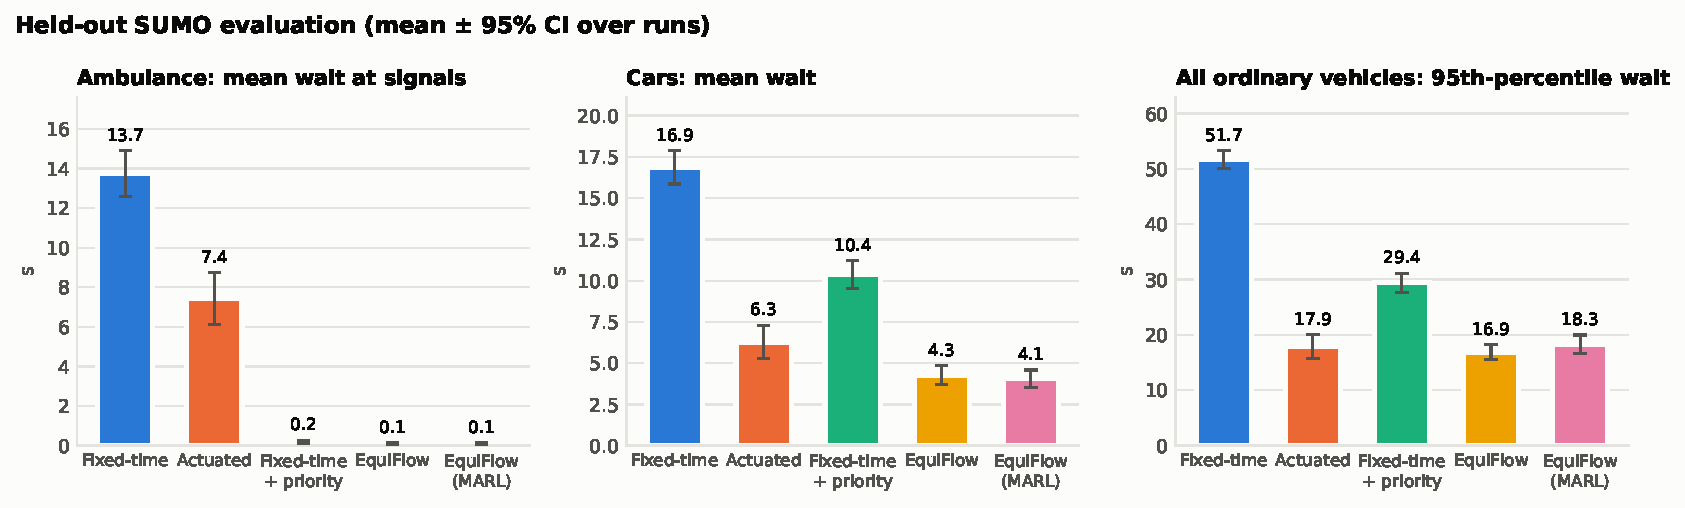
\includegraphics[width=\textwidth]{figures/fig_main_comparison.pdf}
\caption{Held-out evaluation: ambulance wait, car wait and 95th-percentile wait per controller
(mean $\pm$ 95\% CI over 120 runs each).}
\label{fig:it2-main}
\end{figure}

Table~\ref{tab:it2-main} and Figure~\ref{fig:it2-main} give the main comparison. EquiFlow reduces the
ambulance's mean wait at signals from 13.75\,s (fixed-time) and 7.42\,s (actuated) to 0.10\,s, and its travel
time by 16.5\,s (28\%) and 10.1\,s (19\%) respectively. Ordinary traffic also waits less: car wait is 4.28\,s
against 16.87\,s for fixed-time and 6.28\,s for actuated. The paired comparison (Table~\ref{tab:it2-paired})
puts the advantage over actuated at $-2.00 \pm 0.61$\,s (better in 68\% of paired runs), and the worst-served
approach waits 2.3\,s less. The 95th-percentile wait ($-0.96 \pm 1.32$\,s), the longest single wait
($+3.1 \pm 3.3$\,s) and the Jain index across approaches are statistically level with actuated. The price of
priority is paid by the vehicles an ambulance holds: they wait 19.6\,s on average, against 12.4\,s with actuated
control (which never holds them), 25.2\,s with fixed-time plus simple priority and 36.2\,s with fixed-time.

\begin{figure}[htbp]
\centering
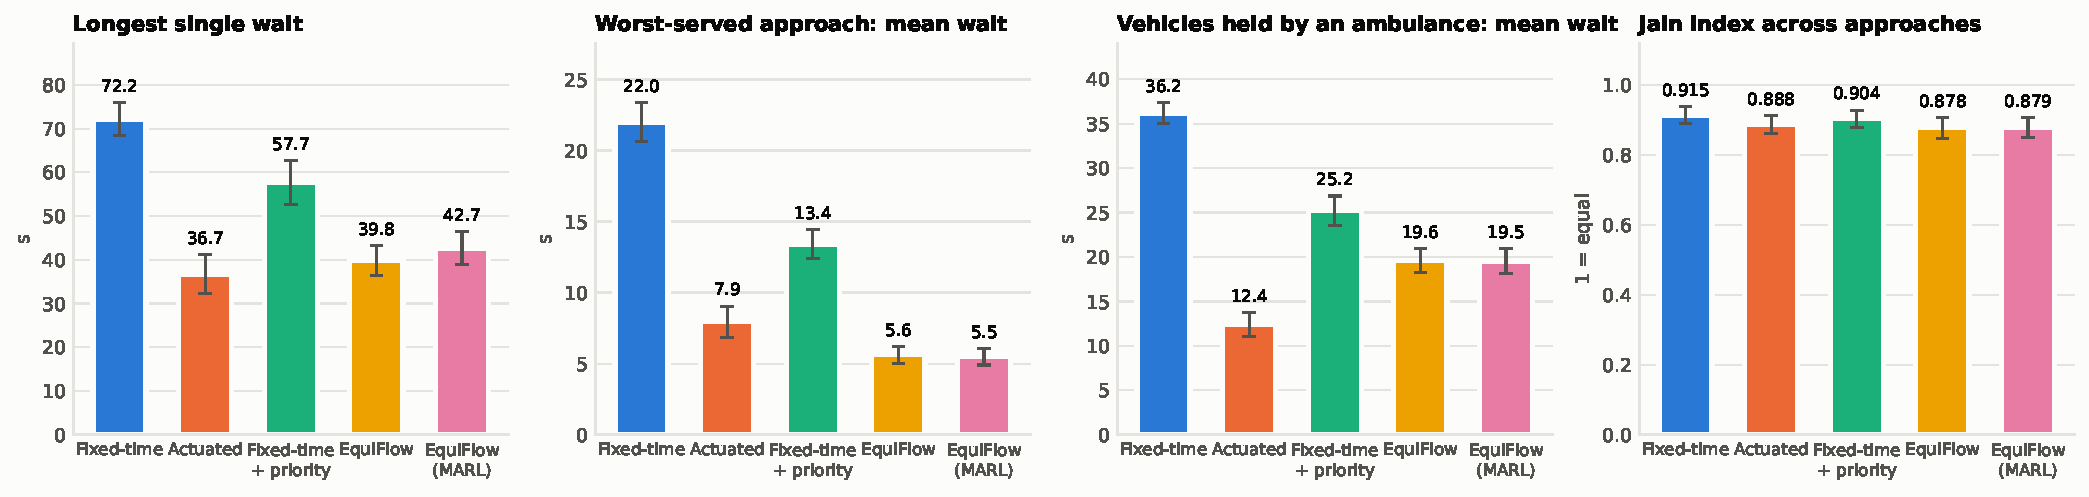
\includegraphics[width=\textwidth]{figures/fig_fairness.pdf}
\caption{Fairness: longest single wait, the worst-served approach's mean wait, the mean wait of the vehicles
held by an ambulance, and Jain's index across approaches.}
\label{fig:it2-fairness}
\end{figure}

\begin{figure}[htbp]
\centering
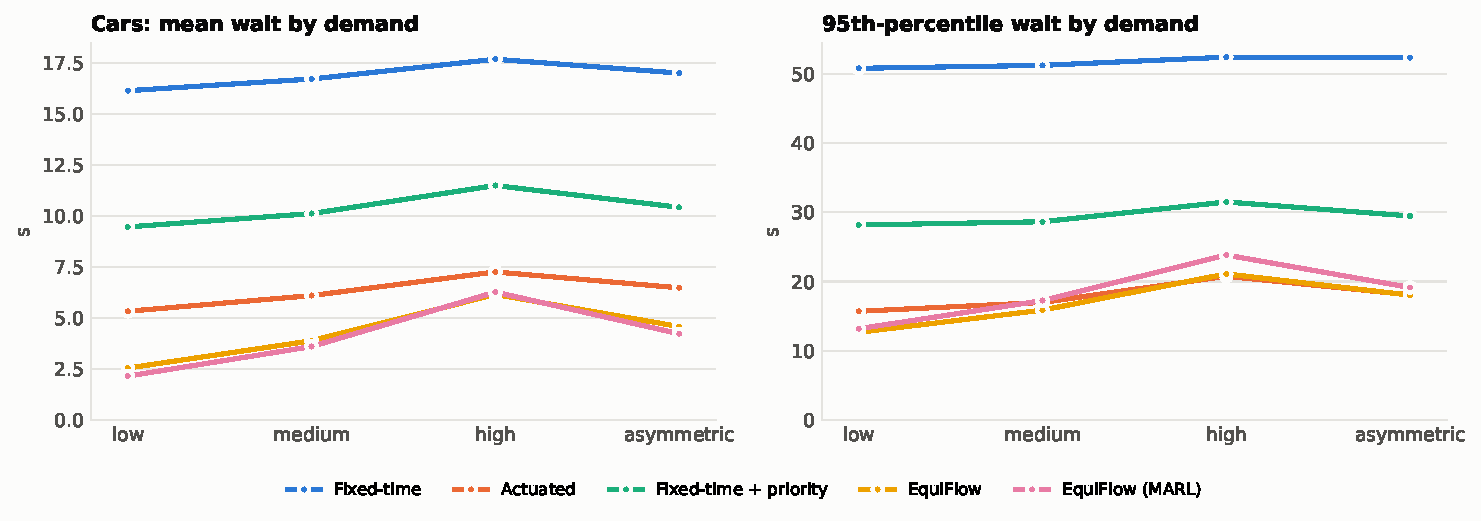
\includegraphics[width=\textwidth]{figures/fig_by_demand.pdf}
\caption{Car mean wait and 95th-percentile wait by demand level.}
\label{fig:it2-demand}
\end{figure}

Under heavy demand (Figure~\ref{fig:it2-demand}) EquiFlow's car wait is below actuated (6.15 against
7.25\,s; 6.92\,s in the first evaluation), and its 95th-percentile wait is now level (21.10 against 20.76\,s, a
paired difference of $+0.33 \pm 2.87$\,s, against $+1.68$\,s in the first evaluation). This is despite every
EquiFlow phase change costing 3\,s of yellow and 2\,s of all-red, against 4\,s of yellow and no all-red in SUMO's
actuated plans; the all-red is kept for safety.

\subsection{Ablations}
\label{sec:it2-ablation}
\begin{figure}[htbp]
\centering
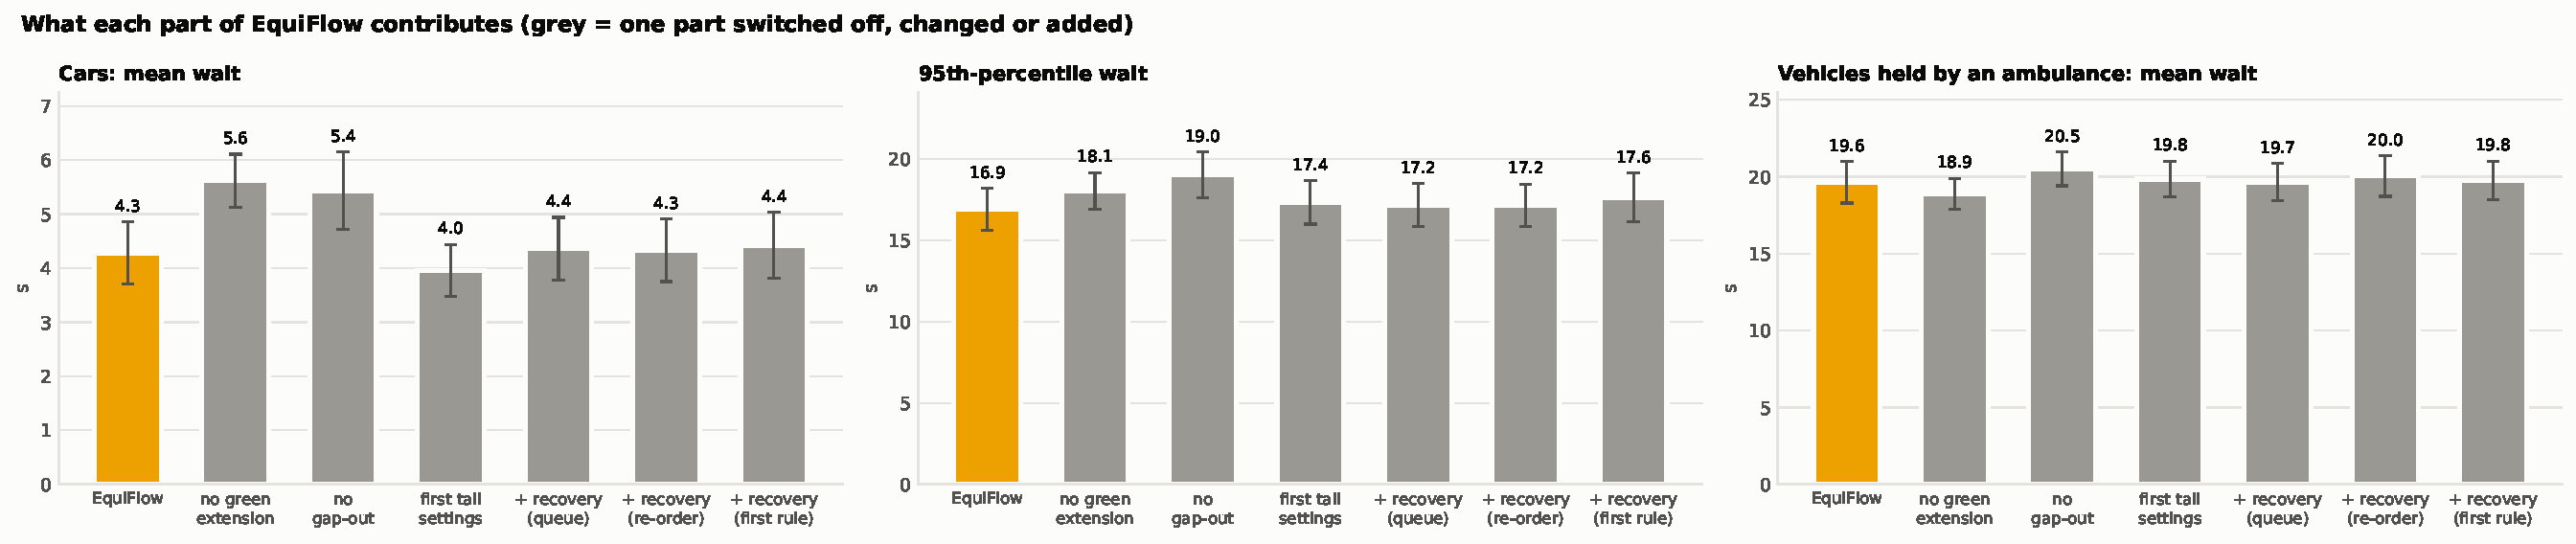
\includegraphics[width=\textwidth]{figures/fig_ablation.pdf}
\caption{Ablations: EquiFlow with one component switched off or replaced.}
\label{fig:it2-ablation}
\end{figure}

Table~\ref{tab:it2-ablation} and Figure~\ref{fig:it2-ablation} switch one component off, change it, or add an
optional one back. \emph{Green extension} gives the largest gain in average waits: without it car wait rises by
1.33\,s (better with it in 95\% of paired runs) and the 95th-percentile wait by 1.16\,s, with no significant
change in the longest wait. In the first evaluation round extension cost 6.6\,s on the longest wait; the tighter
30\,s wait cap and the higher waiting-time weight removed that cost (the first settings have a 4.4\,s longer
longest wait), at 0.3\,s of car wait. \emph{Gap-out} improves every measure: without it car wait rises by 1.15\,s
and the 95th-percentile wait by 2.11\,s (better in 99\% of runs).

\emph{Fair recovery} gives no benefit with any of the three rules. Adding the queue-sized rule raises car wait
by 0.08\,s and the 95th-percentile wait by 0.26\,s; the re-order-only rule changes nothing significantly except a
0.25\,s higher 95th-percentile wait; the first rule is worst (95th percentile +0.74\,s, longest wait +2.2\,s). The
stress scenario (about 40 ambulances per hour, 30 runs per controller) gives the same answer: the queue-sized rule
raises the 95th-percentile wait by 1.3\,s, the first rule by 4.0\,s, and the re-order rule by nothing measurable.
Re-ordering removes the harm but adds no benefit: an adaptive controller that already serves the
longest-waiting busy approach next leaves nothing for a separate recovery phase to fix. Recovery is therefore off
by default.

On the two multi-junction networks (Table~\ref{tab:it2-corridor}) the \emph{green corridor} turns downstream
signals green a little earlier but does not change ambulance travel time, while the vehicles it holds wait
longer: 2.4\,s with the just-in-time rule and 6.8\,s with the first rule. With junctions 300\,m apart, local
priority alone is fast enough, so the corridor is off by default.

\subsection{MARL controller}
\begin{figure}[htbp]
\centering
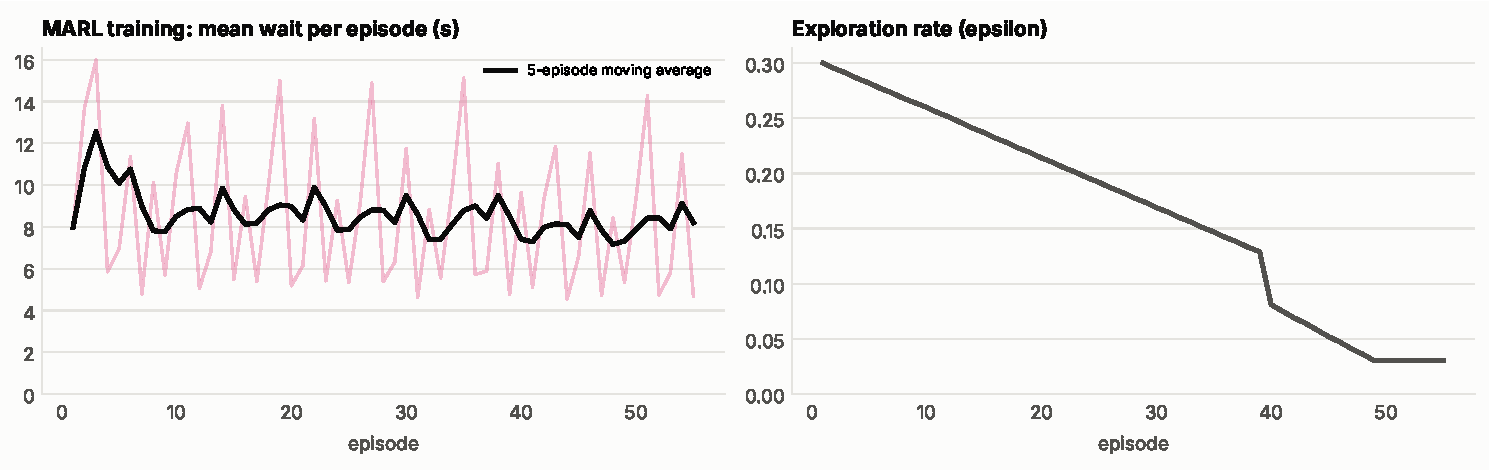
\includegraphics[width=\textwidth]{figures/fig_marl_training.pdf}
\caption{MARL training: mean wait per episode (episodes rotate between networks) and exploration rate.}
\label{fig:it2-marl}
\end{figure}

The first MARL policy (55 training episodes) tied the adaptive heuristic on car wait but had a 1.85\,s higher
95th-percentile wait. Its reward was therefore extended to charge every halted vehicle that has already waited
more than 20\,s (about the 95th-percentile wait), and it was retrained from scratch for 120 episodes on seeds
1--5 with the final junction settings. On the held-out seeds it now beats the heuristic on car wait
($-0.23 \pm 0.18$\,s), but the heuristic's own tail tuning moved further, so MARL's 95th-percentile wait is
$1.43 \pm 0.55$\,s higher and its longest wait 2.9\,s higher, with the same picture on network/demand combinations
it was trained on and on unseen ones (Table~\ref{tab:it2-marl}). The adaptive controller stays the default.

\subsection{Robustness to camera errors}
\begin{figure}[htbp]
\centering
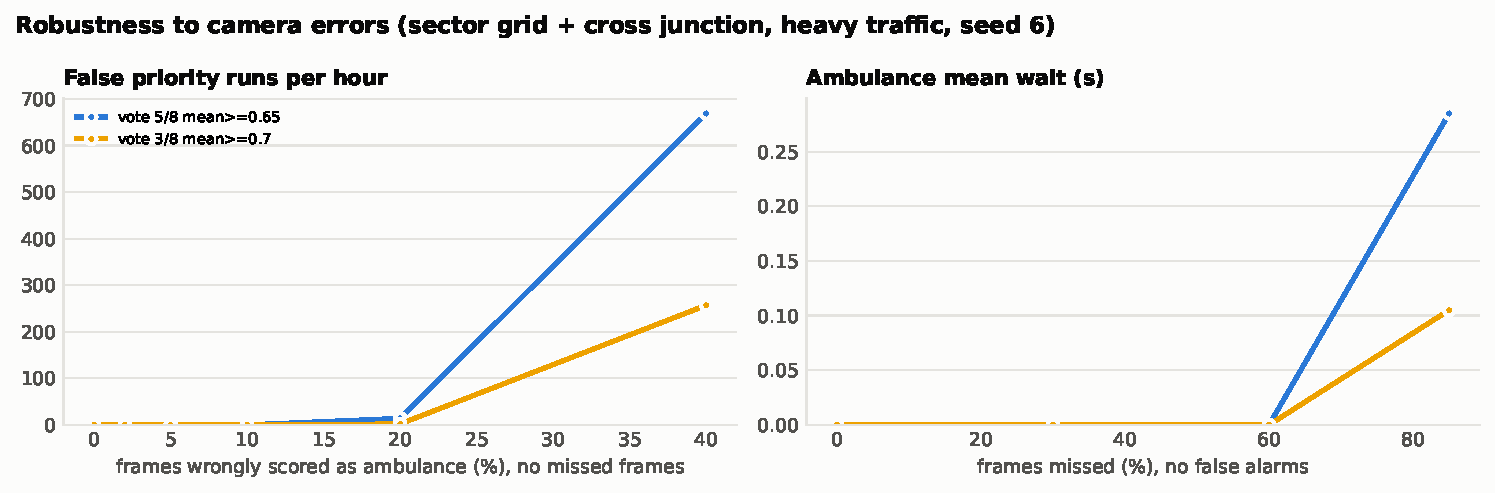
\includegraphics[width=\textwidth]{figures/fig_robustness.pdf}
\caption{False priority runs and ambulance wait as the virtual camera misses frames or scores ordinary
vehicles as ambulances, for the 5-of-8 vote and the live 3-of-8 vote (heavy demand, seed 6).}
\label{fig:it2-robust}
\end{figure}

The sweep was run for both votes (Figure~\ref{fig:it2-robust}). With up to 10\% of frames wrongly scored as
ambulance, neither produces any false priority. At 20\% the 5-of-8 vote (mean $\geq$ 0.65) produces 8--20 false
priority runs per hour and the live 3-of-8 vote (mean $\geq$ 0.70) only 0--4; at 40\% they produce 386--952
and 145--369. The live vote is therefore more tolerant of noisy frames, not less: its stricter mean-score
threshold matters more than the lower vote count. Missing even 85\% of frames barely matters (ambulance wait at
most 0.6\,s). The classifier's per-crop false-alarm rate is 0.9\% on the test split, well inside this margin.

\subsection{Ambulance classifier}
\label{sec:it2-classifier}
\paragraph{Dataset check.} \texttt{Projects/make\_split\_manifest.py} lists all 32\,593 crops with a SHA-1 and a
perceptual hash and looks for images shared between splits. The test split contains no exact copy of a training
image; 134 test crops (3.6\%) are near duplicates of a training crop, all with the same label. The check found
four validation crops labelled ambulance that were copies of training crops labelled other vehicle, and 35
duplicate files inside the training split; all 39 were removed. Removing the four mislabelled copies alone raised
the mid-report model's validation recall from 91.0\% to 91.8\%: all four had been counted as missed ambulances.

\paragraph{Retraining.} Three changes proposed in the mid-report were trained one at a time on the cleaned data and
compared on the validation split only (Table~\ref{tab:it2-cls-val}). Retraining with unchanged settings changes
little; doubling the ambulance crops gives the highest recall but more false alarms; a 128\,px input
(cls\_v5\_img128) is best on PR-AUC and F1 and was selected.

\paragraph{Test split.} Only the selected model and the mid-report model were then run on the held-out test split,
once (Table~\ref{tab:it2-cls-test}). cls\_v5\_img128 is better on every metric: 93.5\% recall at 96.5\% precision
and a 0.9\% false-alarm rate. Recall is lowest on the Pakistani ambulance crops (88.1\%, against 95.9\% on the
public dataset). A threshold chosen on the validation split for 95\% recall gives 95.7\% test recall for the
mid-report model, at 87.7\% precision.

\paragraph{Latency.} On an RTX 4050 laptop GPU the vehicle detector takes 27.7\,ms per 1280\,px frame and the
classifier 1.7\,ms per crop in a batch (Table~\ref{tab:it2-latency}): about 45\,ms per frame, or 22 frames per
second, with ten vehicles in view. Measured back to back, the 128\,px classifier costs the same as the 96\,px one.

\subsection{Tracking on real video}
\label{sec:it2-tracking}
With the new classifier and the old vote (5 of 8, mean $\geq$ 0.65) the pipeline confirmed 5 of the 7 labelled
ambulance passes. \texttt{Projects/tune\_tracking.py} records every track's score per frame once and replays the
vote offline; at the old setting the replay reproduces the pipeline's confirmations exactly on all 12 videos.
Of 360 settings (Table~\ref{tab:it2-tune}), the number of votes K decides the result: every setting with K = 3
and a mean score of 0.70--0.75 confirms all 7 passes with 6 false events, whatever the frame threshold, while
K = 4 or 5 confirm 5. The chosen setting keeps the frame threshold at 0.6 and uses K = 3, mean $\geq$ 0.70.

Table~\ref{tab:it2-tracking} gives the re-run pipeline on all 12 available clips (a thirteenth clip has no source
video): 7 of 7 passes confirmed, on average 0.94\,s after the labelled start, with 6 false confirmations: 3 in
test5, a clip checked to contain no ambulance (a look-alike vehicle), 2 in test12 1.4\,s before a labelled pass,
and 1 in test4. Because the same videos chose and scored the setting, this is optimistic. Choosing the setting on
11 videos and scoring the twelfth, for each video in turn, gives 7 of 7 passes and 11 false events. Seven passes
are far too few for a reliable recall estimate.

\subsection{Performance}
A controller tick takes about 1\,$\mu$s and a MARL decision about 24\,$\mu$s (p99 62\,$\mu$s), against a
100\,000\,$\mu$s tick period (Table~\ref{tab:it2-perf}). A one-hour SUMO run takes about 3\,s.

\section{Failure Analysis}
\begin{table}[htbp]
\centering
\small
\caption{Failure cases found in Iteration 2 and the planned response.}
\label{tab:it2-failures}
\resizebox{\textwidth}{!}{%
\begin{tabular}{lll}
\hline
Failure & Likely cause & Response \\
\hline
Short ambulance tracks missed with a 5-of-8 vote (test12) & too few confident frames before it leaves & resolved: K = 3, re-tuned \\
3 false confirmations in test5 (no ambulance) & ambulance-like vehicle not in training & add its crops as hard negatives \\
Early confirmations (test12, 1.4\,s before the label) & hand-labelled windows are approximate & label from the first visible frame \\
Recall 88\% on Pakistani ambulances (test) & few local ambulance crops in training & collect more local ambulance crops \\
Mislabelled duplicate crops (4 in validation) & copies made while sorting crops & resolved: split manifest + duplicate check \\
False priority at $\geq$20\% per-frame false alarms & vote too permissive for very noisy input & keep per-frame FP $\ll$ 20\%; live 3-of-8 vote is 4$\times$ more tolerant \\
Higher p95 wait than actuated under heavy demand & green length fixed at its start & resolved: extension + tail tuning (gap +0.3\,s, n.s.) \\
Green extension lengthened the longest wait (+6.6\,s) & others held up to the 40\,s cap & resolved: 30\,s cap, wait weight 0.3 \\
Corridor gives no measurable ambulance benefit & junctions 300\,m apart & off by default; just-in-time rule kept as an option \\
Fair recovery gives no benefit (harmful when frequent) & adaptive order already serves delayed approaches & off by default; re-order rule removes the harm \\
MARL better on car wait, worse on tail waits & heuristic tail tuning moved further & longer training, tail-weighted reward \\
\hline
\end{tabular}}
\end{table}

\section{Limitations}
All control results are from simulation; the SUMO cameras are virtual (exact ambulance positions with
simulated classifier scores), so the real camera pipeline and the SUMO evaluation share the controller and the
voting rule but not the video. The live vote (3 of 8) was tuned on the same 12 clips it is scored on, which
hold only 7 ambulance passes. The fair-recovery stress scenario is one synthetic demand pattern. Authentication
is off by default and must be enabled for any deployment.

\section{Iteration Outcome}
The exit criterion is met: the scripted scenario (\texttt{scripts/scripted\_scenario.py}) sends one ambulance,
then two simultaneous ambulances; each is confirmed by detection, receives a protected green, and is followed
by recovery greens, and the whole sequence is recorded in the event log. All 45 automated tests pass. The classifier
was evaluated on the held-out test split and replaced by a better retrained model, all available videos were
processed, and the improvements the first evaluation pointed to were implemented and evaluated on the held-out
seeds: green extension and tail tuning (which closed the heavy-demand gap to actuated control), an approach-level
fairness measure, a re-order-only recovery rule and a recovery stress test, a just-in-time corridor, a retrained
MARL policy and the camera-error sweep for the live vote. Fair recovery and the corridor did not help and are off
by default. The main open items for FYP-2 are reducing the delay of the vehicles an ambulance holds (the cost of
priority that remains), MARL training that also wins on tail waits, more labelled real video, and hard negatives
for ambulance look-alikes.
 after chapter6_iteration1.
% Needs \usepackage{graphicx} (loaded by most report classes).
% All numbers come from sumo/results/heldout/*.csv and the Projects/ evaluation outputs (see docs/RESULTS.md);
% the tables are generated by sumo/latex_tables.py and should be regenerated rather than edited.

\chapter{Iteration 2: Tracking, Control, Integration and Evaluation}
\label{ch:iteration2}

\section{Iteration Objectives}
Iteration~2 turns the perception and simulation work of Iteration~1 into a working, measured system.
Its objectives, taken from the iteration plan, were to:
(i) track ambulances across frames so that a single confident frame cannot trigger priority;
(ii) give a confirmed ambulance a protected green through safe yellow and all-red transitions, also across
neighbouring junctions (green corridor);
(iii) restore service to delayed approaches afterwards (fair recovery) and add a fairness-aware MARL base
controller;
(iv) integrate the modules behind FastAPI and MQTT with a live dashboard; and
(v) evaluate the controllers on repeatable SUMO runs against fixed-time and actuated baselines.
The exit criterion was that a scripted ambulance scenario triggers and completes a logged preemption with
recovery.

\section{Selected Use Cases / Features}
UC-01 (detect an approaching ambulance), UC-02 (estimate traffic state), UC-03 (grant emergency priority),
UC-04 (recover fairly after priority), UC-05 (run a baseline comparison) and UC-06 (monitor the junction on
the dashboard). Requirement coverage after this iteration is summarised in Table~\ref{tab:it2-req}.

\begin{table}[htbp]
\centering
\small
\caption{Functional requirements and test cases addressed in Iteration 2.}
\label{tab:it2-req}
\resizebox{\textwidth}{!}{%
\begin{tabular}{lll}
\hline
Requirement / test & Implementation & Evidence \\
\hline
FR-01--03 detection input, output, logging & \texttt{vision/live.py}, \texttt{eventlog.py} & \texttt{test\_live\_pipeline.py}, CSV event log \\
FR-04 traffic state & SUMO queues; camera approach zones (\texttt{zones:}) & \texttt{test\_fr04\_zone\_...} \\
FR-05 / TC-03 stale detections & 2\,s age limit on external events, K-of-M vote, 60\,s fail-safe & \texttt{test\_tc03\_...} \\
FR-06--08 phases, timing, priority & \texttt{controllers/intersection.py} & \texttt{test\_controller.py} (randomised safety) \\
FR-07 / TC-04 early end of empty green & gap-out after 5\,s, only if another approach has demand & \texttt{test\_tc04\_...} \\
FR-09 / TC-06 logged preemption and recovery & event log + episode table & \texttt{scripts/scripted\_scenario.py} \\
FR-10 recovery uses queue and wait & queue-sized recovery greens, longest wait first & \texttt{test\_fr10\_...} \\
FR-11 baselines & fixed-time, actuated, fixed-time + priority & Section~\ref{sec:it2-results} \\
FR-12 export metrics and configuration & \texttt{run\_manifest.csv} (config + versions per run) & \texttt{results/heldout/} \\
TC-10 repeatability & same seed and configuration give identical results & \texttt{test\_tc10\_...} \\
\hline
\end{tabular}}
\end{table}

\section{Design}
The controller is split into a \emph{base controller} that chooses the next green in normal operation
(fixed-time, adaptive, or the MARL policy) and an \emph{intersection controller} that wraps it with
everything that must never be learned: ambulance priority, minimum green, yellow and all-red, the 90\,s
maximum-wait guard, gap-out and fair recovery. The intersection controller never reads a clock; it is
given the time on every tick, so the same code runs in the live backend (every 0.1\,s) and inside each SUMO
step. Every decision is published as an event on a bus that feeds the REST/WebSocket API, the optional MQTT
bridge and a CSV event log.

\section{Implementation}
\begin{itemize}
\item \textbf{Perception} (\texttt{backend/app/vision/live.py}): YOLO26s vehicle detection with ByteTrack,
the ambulance classifier on each tracked crop (cls\_v5\_img128, retrained in this iteration at 128\,px), and a
confirmation vote over the last 8 frames. The live camera configuration needs 3 ambulance votes (frame score
$\geq$ 0.6) and a mean score of at least 0.70, re-tuned for the new classifier
(Section~\ref{sec:it2-tracking}); the SUMO evaluation and the backend default use 5 of 8 with mean
$\geq$ 0.65. Optional per-approach polygons restrict counting to the lanes that queue for the signal and
report stationary vehicles as the queue.
\item \textbf{Signal control} (\texttt{backend/app/controllers/}): base controllers, the MARL policy
(shared Q-network over per-phase features, pure NumPy) and the intersection controller described above.
\item \textbf{Integration} (\texttt{backend/app/}): FastAPI REST + WebSocket + MJPEG, MQTT topics, a live
SUMO view driven through TraCI, an optional API key on every write endpoint, and the CSV event log.
\item \textbf{Evaluation} (\texttt{sumo/}): \texttt{run\_matrix.py} runs every controller on the same
networks, demand levels and seeds in parallel; \texttt{aggregate.py} computes means, confidence intervals and
paired differences; \texttt{make\_plots.py} and \texttt{latex\_tables.py} produce the figures and tables in
this chapter.
\end{itemize}

\section{Algorithms and Technical Decisions}
\paragraph{Gap-out.} A green that has run at least 5\,s ends early when no vehicle is within 120\,m of its
stop line and another approach has demand. It is never applied during priority and always passes through
the full yellow and all-red.
\paragraph{Green extension.} Actuated control lengthens a green vehicle by vehicle, while the adaptive controller
fixes each green's length when it starts. A base-controller green that reaches its planned length therefore keeps
going while its approach is still at least as busy as every other one, up to 45\,s, and only while no other
approach with a queue has waited 30\,s. To keep the tail of the waiting-time distribution short, the adaptive
controller also weights waiting time more when it chooses the next green (weight 0.3 instead of 0.1). It is never applied during priority or recovery, and every green still
ends through the full yellow and all-red. The two limits were chosen on tuning seeds 1--2, not on the held-out
seeds.
\paragraph{Priority.} After the vote confirms an ambulance, the current green finishes its minimum time,
then yellow and all-red, and the ambulance's approach turns green alone. Priority ends 4\,s after the
ambulance was last seen, or after 60\,s as a fail-safe. Two ambulances are served first come, first served.
\paragraph{Fair recovery.} After priority, the approaches that were held red and have a queue are served in
order of longest wait, each for about as long as its queue needs to clear (2\,s per queued vehicle, at least
5\,s, at most 30\,s). A first version gave every delayed approach a fixed 15\,s green plus extra, and a third
rule only re-orders the delayed approaches and leaves each green's length to the base controller. Because none of
them improved on having no recovery (Section~\ref{sec:it2-ablation}), recovery is off by default and kept as an
option; the scripted exit scenario switches it on to verify the logged recovery sequence.
\paragraph{Green corridor.} Once a camera confirms an ambulance, signals further along its route are asked for
priority \emph{just in time}: only when the ambulance's arrival time is within the time that signal needs to
switch to it (minimum green, yellow and all-red) plus 3\,s, or, if its phase is already green, when that green
would otherwise end just before the ambulance arrives. The first version cleared every signal within 25\,s of
arrival. Neither made ambulances faster on the evaluated networks, so the corridor is off by default.
\paragraph{Stale detections.} An externally reported detection older than 2\,s (or more than 2\,s in the
future) is rejected and logged, so a delayed or replayed message cannot request priority.

\section{Evaluation Set-up}
Six signalised Islamabad junction networks were each run at four demand levels for one simulated hour.
Every controller used the same 120 network/demand/seed combinations with seeds 6--10; the MARL policy was
trained on seeds 1--5, so all evaluation runs are held out. Ambulances are confirmed by a virtual camera per
approach using the real voting rule. Results are reported as mean $\pm$ 95\% confidence interval over runs,
and as \emph{paired} differences on identical runs, which removes the large differences between networks.
Besides network-wide waits, an approach-level measure counts the vehicles an ambulance actually holds: ordinary
vehicles stopped at a junction while a real ambulance is within camera range on another of its approaches. It is
ground truth, so it is measured the same way for controllers that give no priority. A stress scenario (heavy
traffic and about 40 ambulances per hour, three times the heavy level) tests fair recovery separately.

% Generated by sumo/latex_tables.py from the CSV results. Do not edit by hand; re-run the script.

\begin{table}[htbp]
\centering
\small
\caption{Held-out evaluation: mean $\pm$ 95\% confidence interval over one-hour SUMO runs (seeds 6--10).}
\label{tab:it2-main}
\resizebox{\textwidth}{!}{%
\begin{tabular}{lccccc}
\hline
Metric & Fixed-time & Actuated & Fixed + priority & EquiFlow & EquiFlow (MARL) \\
\hline
Car mean wait (s) & 16.87 $\pm$ 1.02 & 6.28 $\pm$ 1.01 & 10.36 $\pm$ 0.86 & 4.28 $\pm$ 0.57 & 4.05 $\pm$ 0.53 \\
Ordinary vehicles, mean wait (s) & 17.07 $\pm$ 1.05 & 6.23 $\pm$ 0.99 & 10.29 $\pm$ 0.84 & 4.32 $\pm$ 0.56 & 4.10 $\pm$ 0.52 \\
95th-percentile wait (s) & 51.71 $\pm$ 1.61 & 17.87 $\pm$ 2.13 & 29.44 $\pm$ 1.69 & 16.91 $\pm$ 1.31 & 18.34 $\pm$ 1.65 \\
Longest single wait (s) & 72.17 $\pm$ 3.72 & 36.71 $\pm$ 4.45 & 57.69 $\pm$ 5.03 & 39.84 $\pm$ 3.34 & 42.69 $\pm$ 3.72 \\
Share waiting $>$60 s & 0.030 $\pm$ 0.005 & 0.002 $\pm$ 0.001 & 0.002 $\pm$ 0.001 & 0.001 $\pm$ 0.000 & 0.001 $\pm$ 0.001 \\
Worst approach, mean wait (s) & 21.98 $\pm$ 1.37 & 7.95 $\pm$ 1.10 & 13.40 $\pm$ 1.01 & 5.63 $\pm$ 0.59 & 5.49 $\pm$ 0.58 \\
Jain index across approaches & 0.915 $\pm$ 0.025 & 0.888 $\pm$ 0.025 & 0.904 $\pm$ 0.025 & 0.878 $\pm$ 0.030 & 0.879 $\pm$ 0.029 \\
Held by an ambulance, mean wait (s) & 36.17 $\pm$ 1.16 & 12.39 $\pm$ 1.37 & 25.22 $\pm$ 1.63 & 19.64 $\pm$ 1.35 & 19.55 $\pm$ 1.43 \\
Held by an ambulance, p95 wait (s) & 56.02 $\pm$ 2.19 & 22.53 $\pm$ 3.00 & 39.74 $\pm$ 3.26 & 29.47 $\pm$ 2.18 & 31.80 $\pm$ 3.17 \\
Ambulance mean wait (s) & 13.75 $\pm$ 1.16 & 7.42 $\pm$ 1.31 & 0.19 $\pm$ 0.08 & 0.10 $\pm$ 0.06 & 0.10 $\pm$ 0.05 \\
Ambulance travel time (s) & 59.14 $\pm$ 2.42 & 52.75 $\pm$ 2.40 & 43.19 $\pm$ 2.21 & 42.68 $\pm$ 2.22 & 42.54 $\pm$ 2.22 \\
Detection to green (s) & -- & -- & 2.57 $\pm$ 0.17 & 2.37 $\pm$ 0.13 & 2.39 $\pm$ 0.16 \\
Recovery interval (s) & -- & -- & 0.00 $\pm$ 0.00 & 0.00 $\pm$ 0.00 & 0.00 $\pm$ 0.00 \\
Runs & 120 & 120 & 120 & 120 & 120 \\
\hline
\end{tabular}}
\end{table}

\begin{table}[htbp]
\centering
\small
\caption{Ablations: EquiFlow with one component switched off, changed or added (all networks).}
\label{tab:it2-ablation}
\resizebox{\textwidth}{!}{%
\begin{tabular}{lccccccc}
\hline
Metric & EquiFlow & No extension & No gap-out & First tail settings & + Recovery (queue) & + Recovery (re-order) & + Recovery (first rule) \\
\hline
Car mean wait (s) & 4.28 $\pm$ 0.57 & 5.62 $\pm$ 0.49 & 5.43 $\pm$ 0.71 & 3.96 $\pm$ 0.48 & 4.36 $\pm$ 0.58 & 4.33 $\pm$ 0.58 & 4.42 $\pm$ 0.61 \\
95th-percentile wait (s) & 16.91 $\pm$ 1.31 & 18.07 $\pm$ 1.12 & 19.02 $\pm$ 1.41 & 17.35 $\pm$ 1.34 & 17.17 $\pm$ 1.32 & 17.16 $\pm$ 1.31 & 17.65 $\pm$ 1.49 \\
Longest single wait (s) & 39.84 $\pm$ 3.34 & 38.48 $\pm$ 3.82 & 42.21 $\pm$ 3.22 & 44.19 $\pm$ 3.08 & 39.78 $\pm$ 3.32 & 40.31 $\pm$ 3.60 & 41.99 $\pm$ 3.90 \\
Jain index across approaches & 0.878 $\pm$ 0.030 & 0.911 $\pm$ 0.025 & 0.889 $\pm$ 0.029 & 0.864 $\pm$ 0.032 & 0.881 $\pm$ 0.030 & 0.880 $\pm$ 0.030 & 0.877 $\pm$ 0.030 \\
Held by an ambulance, mean wait (s) & 19.64 $\pm$ 1.35 & 18.89 $\pm$ 1.00 & 20.50 $\pm$ 1.09 & 19.84 $\pm$ 1.17 & 19.66 $\pm$ 1.21 & 20.04 $\pm$ 1.32 & 19.77 $\pm$ 1.24 \\
Ambulance mean wait (s) & 0.10 $\pm$ 0.06 & 0.13 $\pm$ 0.06 & 0.14 $\pm$ 0.08 & 0.10 $\pm$ 0.04 & 0.10 $\pm$ 0.05 & 0.10 $\pm$ 0.06 & 0.08 $\pm$ 0.03 \\
Ambulance travel time (s) & 42.68 $\pm$ 2.22 & 42.92 $\pm$ 2.22 & 42.82 $\pm$ 2.22 & 42.57 $\pm$ 2.22 & 42.65 $\pm$ 2.22 & 42.66 $\pm$ 2.22 & 42.63 $\pm$ 2.21 \\
Recovery interval (s) & 0.00 $\pm$ 0.00 & 0.00 $\pm$ 0.00 & 0.00 $\pm$ 0.00 & 0.00 $\pm$ 0.00 & 22.94 $\pm$ 0.94 & 21.61 $\pm$ 0.88 & 28.25 $\pm$ 1.35 \\
Runs & 120 & 120 & 120 & 120 & 120 & 120 & 120 \\
\hline
\end{tabular}}
\end{table}

\begin{table}[htbp]
\centering
\small
\caption{Green corridor on the two multi-junction networks (sector grid, diamond): EquiFlow (no corridor) minus EquiFlow with each corridor rule, on identical runs. Negative = EquiFlow lower. $^*$: the 95\% CI excludes zero.}
\label{tab:it2-corridor}
\begin{tabular}{llccc}
\hline
Versus & Metric & Difference (95\% CI) & EquiFlow better in & Runs \\
\hline
+ Corridor (just in time) & Car mean wait (s) & -0.06 $\pm$ 0.07 & 40\% & 40 \\
+ Corridor (just in time) & 95th-percentile wait (s) & -0.37 $\pm$ 0.32$^*$ & 32\% & 40 \\
+ Corridor (just in time) & Longest single wait (s) & -0.17 $\pm$ 1.30 & 22\% & 40 \\
+ Corridor (just in time) & Held by an ambulance, mean wait (s) & -2.43 $\pm$ 1.31$^*$ & 63\% & 35 \\
+ Corridor (just in time) & Ambulance mean wait (s) & -0.02 $\pm$ 0.03 & 8\% & 40 \\
+ Corridor (just in time) & Ambulance travel time (s) & +0.04 $\pm$ 0.12 & 18\% & 40 \\
+ Corridor (25 s ETA) & Car mean wait (s) & -0.06 $\pm$ 0.07 & 55\% & 40 \\
+ Corridor (25 s ETA) & 95th-percentile wait (s) & -0.71 $\pm$ 0.47$^*$ & 52\% & 40 \\
+ Corridor (25 s ETA) & Longest single wait (s) & -4.33 $\pm$ 2.17$^*$ & 60\% & 40 \\
+ Corridor (25 s ETA) & Held by an ambulance, mean wait (s) & -6.76 $\pm$ 1.92$^*$ & 91\% & 35 \\
+ Corridor (25 s ETA) & Ambulance mean wait (s) & -0.01 $\pm$ 0.02 & 2\% & 40 \\
+ Corridor (25 s ETA) & Ambulance travel time (s) & +0.08 $\pm$ 0.11 & 20\% & 40 \\
\hline
\end{tabular}
\end{table}

\begin{table}[htbp]
\centering
\small
\caption{Paired comparison on identical runs (same network, demand and seed): EquiFlow minus the other controller. Negative values mean EquiFlow is lower. $^*$: the 95\% CI excludes zero.}
\label{tab:it2-paired}
\begin{tabular}{llccc}
\hline
Versus & Metric & Difference (95\% CI) & EquiFlow better in & Runs \\
\hline
Fixed-time & Car mean wait (s) & -12.59 $\pm$ 0.66$^*$ & 100\% & 120 \\
Fixed-time & 95th-percentile wait (s) & -34.80 $\pm$ 1.19$^*$ & 100\% & 120 \\
Fixed-time & Longest single wait (s) & -32.33 $\pm$ 3.77$^*$ & 97\% & 120 \\
Fixed-time & Ambulance mean wait (s) & -13.64 $\pm$ 1.13$^*$ & 100\% & 120 \\
Actuated & Car mean wait (s) & -2.00 $\pm$ 0.61$^*$ & 68\% & 120 \\
Actuated & 95th-percentile wait (s) & -0.96 $\pm$ 1.32 & 48\% & 120 \\
Actuated & Longest single wait (s) & +3.13 $\pm$ 3.28 & 30\% & 120 \\
Actuated & Ambulance mean wait (s) & -7.32 $\pm$ 1.29$^*$ & 99\% & 120 \\
Fixed + priority & Car mean wait (s) & -6.08 $\pm$ 0.42$^*$ & 100\% & 120 \\
Fixed + priority & 95th-percentile wait (s) & -12.53 $\pm$ 0.82$^*$ & 100\% & 120 \\
Fixed + priority & Longest single wait (s) & -17.85 $\pm$ 3.19$^*$ & 85\% & 120 \\
Fixed + priority & Ambulance mean wait (s) & -0.09 $\pm$ 0.06$^*$ & 28\% & 120 \\
EquiFlow (MARL) & Car mean wait (s) & +0.23 $\pm$ 0.18$^*$ & 48\% & 120 \\
EquiFlow (MARL) & 95th-percentile wait (s) & -1.43 $\pm$ 0.55$^*$ & 60\% & 120 \\
EquiFlow (MARL) & Longest single wait (s) & -2.85 $\pm$ 1.97$^*$ & 62\% & 120 \\
EquiFlow (MARL) & Ambulance mean wait (s) & +0.01 $\pm$ 0.05 & 12\% & 120 \\
No gap-out & Car mean wait (s) & -1.15 $\pm$ 0.18$^*$ & 99\% & 120 \\
No gap-out & 95th-percentile wait (s) & -2.11 $\pm$ 0.27$^*$ & 91\% & 120 \\
No gap-out & Longest single wait (s) & -2.37 $\pm$ 1.94$^*$ & 60\% & 120 \\
No gap-out & Ambulance mean wait (s) & -0.04 $\pm$ 0.05 & 17\% & 120 \\
No extension & Car mean wait (s) & -1.33 $\pm$ 0.18$^*$ & 95\% & 120 \\
No extension & 95th-percentile wait (s) & -1.16 $\pm$ 0.38$^*$ & 59\% & 120 \\
No extension & Longest single wait (s) & +1.36 $\pm$ 2.00 & 32\% & 120 \\
No extension & Ambulance mean wait (s) & -0.03 $\pm$ 0.04 & 21\% & 120 \\
First tail settings & Car mean wait (s) & +0.32 $\pm$ 0.13$^*$ & 34\% & 120 \\
First tail settings & 95th-percentile wait (s) & -0.44 $\pm$ 0.29$^*$ & 41\% & 120 \\
First tail settings & Longest single wait (s) & -4.35 $\pm$ 2.09$^*$ & 62\% & 120 \\
First tail settings & Ambulance mean wait (s) & +0.00 $\pm$ 0.05 & 11\% & 120 \\
+ Recovery (queue) & Car mean wait (s) & -0.08 $\pm$ 0.07$^*$ & 59\% & 120 \\
+ Recovery (queue) & 95th-percentile wait (s) & -0.26 $\pm$ 0.21$^*$ & 46\% & 120 \\
+ Recovery (queue) & Longest single wait (s) & +0.06 $\pm$ 1.72 & 42\% & 120 \\
+ Recovery (queue) & Ambulance mean wait (s) & +0.00 $\pm$ 0.03 & 9\% & 120 \\
+ Recovery (re-order) & Car mean wait (s) & -0.05 $\pm$ 0.06 & 53\% & 120 \\
+ Recovery (re-order) & 95th-percentile wait (s) & -0.25 $\pm$ 0.18$^*$ & 40\% & 120 \\
+ Recovery (re-order) & Longest single wait (s) & -0.47 $\pm$ 1.58 & 33\% & 120 \\
+ Recovery (re-order) & Ambulance mean wait (s) & +0.00 $\pm$ 0.04 & 3\% & 120 \\
+ Recovery (first rule) & Car mean wait (s) & -0.14 $\pm$ 0.09$^*$ & 59\% & 120 \\
+ Recovery (first rule) & 95th-percentile wait (s) & -0.74 $\pm$ 0.34$^*$ & 45\% & 120 \\
+ Recovery (first rule) & Longest single wait (s) & -2.15 $\pm$ 1.81$^*$ & 48\% & 120 \\
+ Recovery (first rule) & Ambulance mean wait (s) & +0.02 $\pm$ 0.05 & 8\% & 120 \\
\hline
\end{tabular}
\end{table}

\begin{table}[htbp]
\centering
\small
\caption{MARL minus adaptive EquiFlow on identical runs, split by whether the network/demand combination was used in MARL training. All seeds are unseen. Negative = MARL lower.}
\label{tab:it2-marl}
\begin{tabular}{lcc}
\hline
Metric & Trained combinations & Unseen combinations \\
\hline
Car mean wait (s) & -0.23 $\pm$ 0.27 (n=40) & -0.23 $\pm$ 0.24 (n=80) \\
95th-percentile wait (s) & +0.84 $\pm$ 0.54 (n=40) & +1.73 $\pm$ 0.77 (n=80) \\
Jain index across approaches & +0.001 $\pm$ 0.011 (n=40) & +0.001 $\pm$ 0.010 (n=80) \\
Ambulance mean wait (s) & +0.00 $\pm$ 0.03 (n=40) & -0.01 $\pm$ 0.07 (n=80) \\
\hline
\end{tabular}
\end{table}

\begin{table}[htbp]
\centering
\small
\caption{Signal controller timing on one CPU core (sumo/benchmark.py). The live backend ticks every 100\,000\,$\mu$s.}
\label{tab:it2-perf}
\begin{tabular}{lcccc}
\hline
Measured & Mean ($\mu$s) & Median & p99 & Max \\
\hline
tick (fixed\_time) & 0.94 & 0.92 & 3.21 & 99.37 \\
decision (fixed\_time) & 0.42 & 0.38 & 0.63 & 467.97 \\
tick (adaptive) & 1.07 & 0.95 & 3.77 & 680.95 \\
decision (adaptive) & 1.39 & 1.2 & 2.68 & 935.52 \\
tick (marl) & 1.35 & 0.94 & 5.07 & 173.0 \\
decision (marl) & 23.83 & 19.82 & 61.69 & 4408.28 \\
\hline
\end{tabular}
\end{table}

\begin{table}[htbp]
\centering
\small
\caption{Tracking pipeline (YOLO26s + ByteTrack + cls\_v5\_img128, 3-of-8 vote with mean score $\geq$ 0.70) on the Islamabad videos. A pass counts as detected if confirmed within 1\,s of its hand-labelled window.}
\label{tab:it2-tracking}
\begin{tabular}{lcccccc}
\hline
Video & Crops used in & Passes & Detected & Missed & False events & Latency (s) \\
\hline
test1 & no & 1 & 1 & 0 & 0 & 0.48 \\
test11 & test & 0 & 0 & 0 & 0 & -- \\
test12 & no & 3 & 3 & 0 & 2 & 2.00 0.00 0.60 \\
test2 & no & 1 & 1 & 0 & 0 & 0.07 \\
test3 & no & 1 & 1 & 0 & 0 & 3.37 \\
test4 & no & 1 & 1 & 0 & 1 & 0.07 \\
test5 & no & 0 & 0 & 0 & 3 & -- \\
test6 & train & 0 & 0 & 0 & 0 & -- \\
test8 & train & 0 & 0 & 0 & 0 & -- \\
test9 & val & 0 & 0 & 0 & 0 & -- \\
v1 & train & 0 & 0 & 0 & 0 & -- \\
v2 & train & 0 & 0 & 0 & 0 & -- \\
\hline
\end{tabular}
\end{table}

\begin{table}[htbp]
\centering
\small
\caption{Ambulance classifier on the held-out test split (Projects/eval\_detector.py, threshold 0.5; 768 ambulance and 2\,953 other-vehicle crops).}
\label{tab:it2-cls-test}
\begin{tabular}{lccccccc}
\hline
Model & Accuracy & Precision & Recall & F1 & False alarms & ROC-AUC & PR-AUC \\
\hline
cls\_v4-2 (mid-report) & 97.7\% & 95.7\% & 92.8\% & 0.942 & 1.1\% & 0.993 & 0.981 \\
cls\_v5\_img128 (pipeline) & 98.0\% & 96.5\% & 93.5\% & 0.950 & 0.9\% & 0.995 & 0.985 \\
\hline
\end{tabular}
\end{table}

\begin{table}[htbp]
\centering
\small
\caption{Classifier training runs on the cleaned validation split (yolo26n-cls, 30 epochs; Projects/train\_cls\_v5.py). The model was chosen here and then run once on the test split.}
\label{tab:it2-cls-val}
\begin{tabular}{llccccc}
\hline
Run & Change & PR-AUC & Recall & Precision & F1 & False alarms \\
\hline
cls\_v4-2 & mid-report model & 0.973 & 91.8\% & 95.6\% & 0.937 & 0.7\% \\
cls\_v5\_base & same settings, cleaned data & 0.975 & 91.8\% & 94.5\% & 0.931 & 0.8\% \\
cls\_v5\_img128 & input 128\,px & 0.979 & 92.8\% & 95.0\% & 0.939 & 0.8\% \\
cls\_v5\_os2 & ambulance crops $\times$2 & 0.975 & 93.7\% & 92.8\% & 0.933 & 1.1\% \\
\hline
\end{tabular}
\end{table}

\begin{table}[htbp]
\centering
\small
\caption{Re-tuning the confirmation vote for cls\_v5\_img128 on the 12 Islamabad videos (Projects/tune\_tracking.py, 360 settings replayed offline; window M = 8 frames).}
\label{tab:it2-tune}
\begin{tabular}{lcccccc}
\hline
Setting & Frame threshold & Mean score & K of 8 & Passes detected & False events & Latency (s) \\
\hline
before & 0.6 & 0.65 & 5 & 5 of 7 & 6 & 0.99 \\
after & 0.6 & 0.7 & 3 & 7 of 7 & 6 & 0.94 \\
\hline
\end{tabular}
\end{table}

\begin{table}[htbp]
\centering
\small
\caption{Perception latency on an RTX 4050 laptop GPU (Projects/eval\_detector.py, a real 1280\,px video frame).}
\label{tab:it2-latency}
\begin{tabular}{lccc}
\hline
Stage & Mean (ms) & Median (ms) & p95 (ms) \\
\hline
YOLO26s vehicle detector, one frame & 27.71 & 26.93 & 32.01 \\
classifier, one crop & 7.94 & 7.53 & 10.65 \\
classifier, batch of 16 crops (1.71\,ms per crop) & 27.4 & 26.78 & 33.74 \\
\hline
full pipeline, 10 vehicles in view (estimate) & 44.8 & & \\
\hline
\end{tabular}
\end{table}



\section{Results}
\label{sec:it2-results}
\begin{figure}[htbp]
\centering
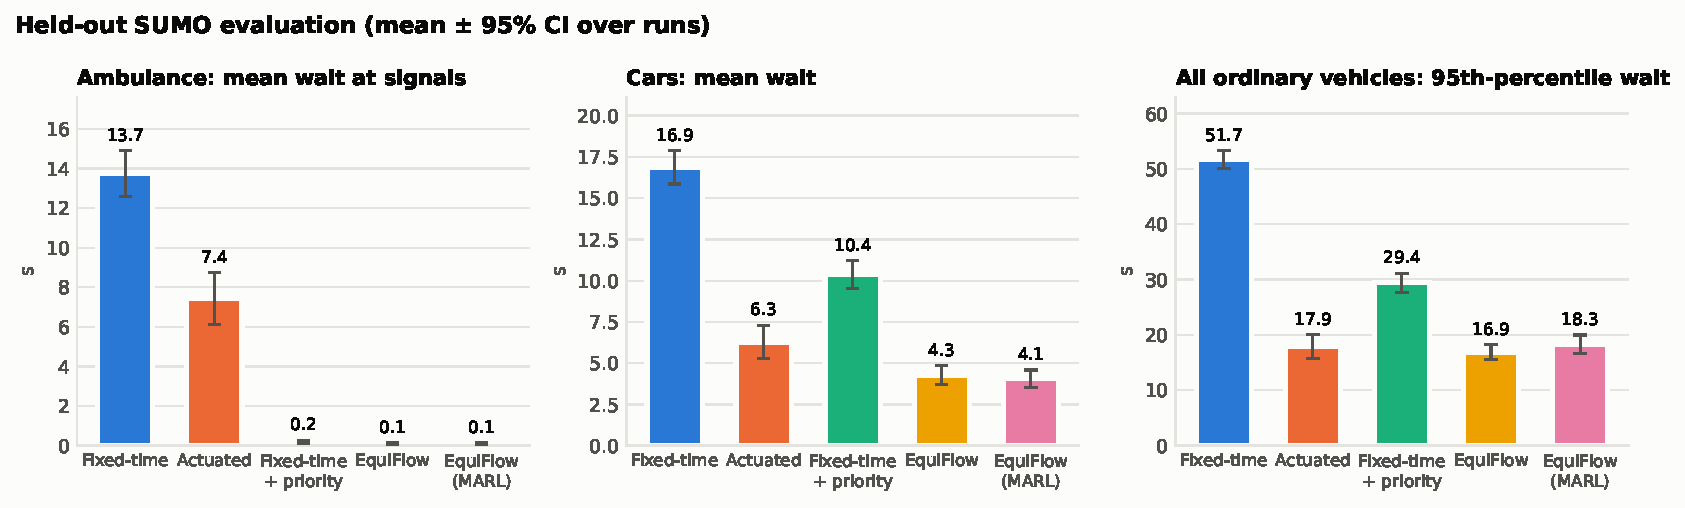
\includegraphics[width=\textwidth]{figures/fig_main_comparison.pdf}
\caption{Held-out evaluation: ambulance wait, car wait and 95th-percentile wait per controller
(mean $\pm$ 95\% CI over 120 runs each).}
\label{fig:it2-main}
\end{figure}

Table~\ref{tab:it2-main} and Figure~\ref{fig:it2-main} give the main comparison. EquiFlow reduces the
ambulance's mean wait at signals from 13.75\,s (fixed-time) and 7.42\,s (actuated) to 0.10\,s, and its travel
time by 16.5\,s (28\%) and 10.1\,s (19\%) respectively. Ordinary traffic also waits less: car wait is 4.28\,s
against 16.87\,s for fixed-time and 6.28\,s for actuated. The paired comparison (Table~\ref{tab:it2-paired})
puts the advantage over actuated at $-2.00 \pm 0.61$\,s (better in 68\% of paired runs), and the worst-served
approach waits 2.3\,s less. The 95th-percentile wait ($-0.96 \pm 1.32$\,s), the longest single wait
($+3.1 \pm 3.3$\,s) and the Jain index across approaches are statistically level with actuated. The price of
priority is paid by the vehicles an ambulance holds: they wait 19.6\,s on average, against 12.4\,s with actuated
control (which never holds them), 25.2\,s with fixed-time plus simple priority and 36.2\,s with fixed-time.

\begin{figure}[htbp]
\centering
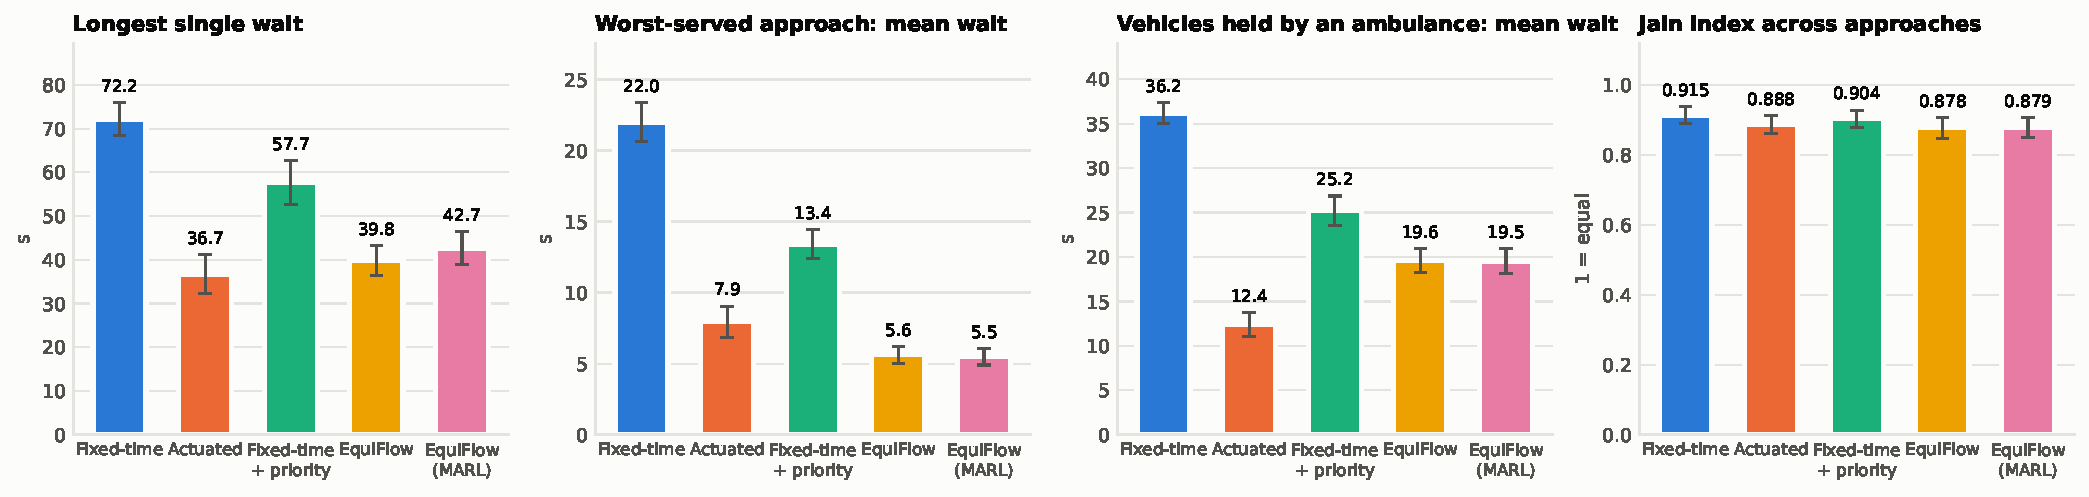
\includegraphics[width=\textwidth]{figures/fig_fairness.pdf}
\caption{Fairness: longest single wait, the worst-served approach's mean wait, the mean wait of the vehicles
held by an ambulance, and Jain's index across approaches.}
\label{fig:it2-fairness}
\end{figure}

\begin{figure}[htbp]
\centering
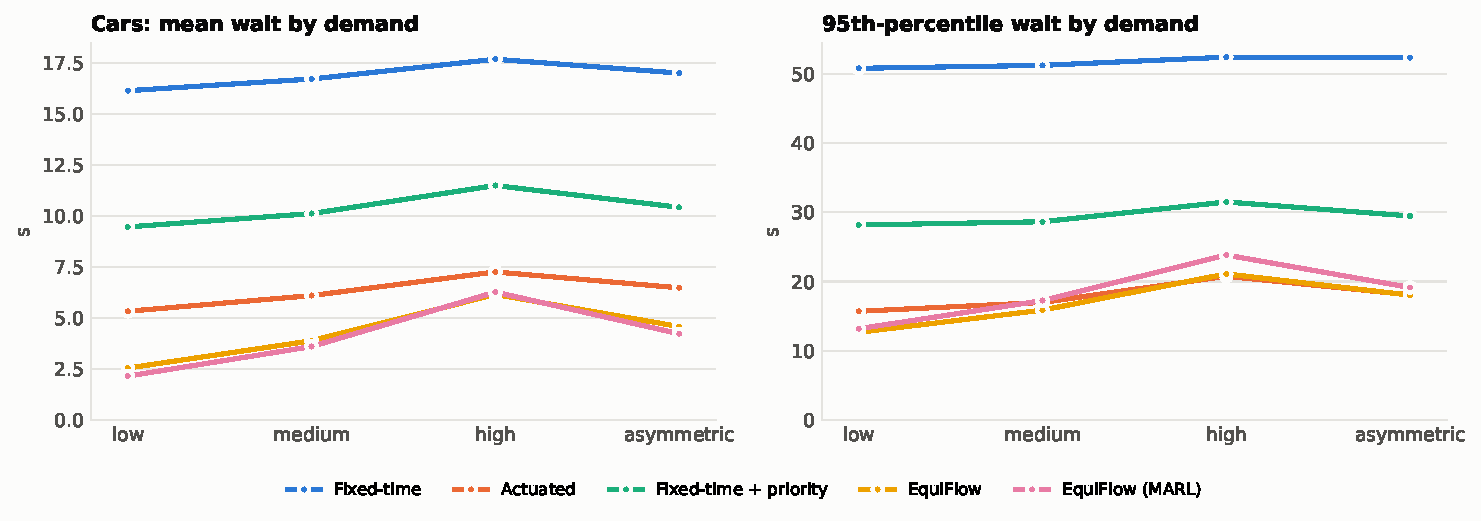
\includegraphics[width=\textwidth]{figures/fig_by_demand.pdf}
\caption{Car mean wait and 95th-percentile wait by demand level.}
\label{fig:it2-demand}
\end{figure}

Under heavy demand (Figure~\ref{fig:it2-demand}) EquiFlow's car wait is below actuated (6.15 against
7.25\,s; 6.92\,s in the first evaluation), and its 95th-percentile wait is now level (21.10 against 20.76\,s, a
paired difference of $+0.33 \pm 2.87$\,s, against $+1.68$\,s in the first evaluation). This is despite every
EquiFlow phase change costing 3\,s of yellow and 2\,s of all-red, against 4\,s of yellow and no all-red in SUMO's
actuated plans; the all-red is kept for safety.

\subsection{Ablations}
\label{sec:it2-ablation}
\begin{figure}[htbp]
\centering
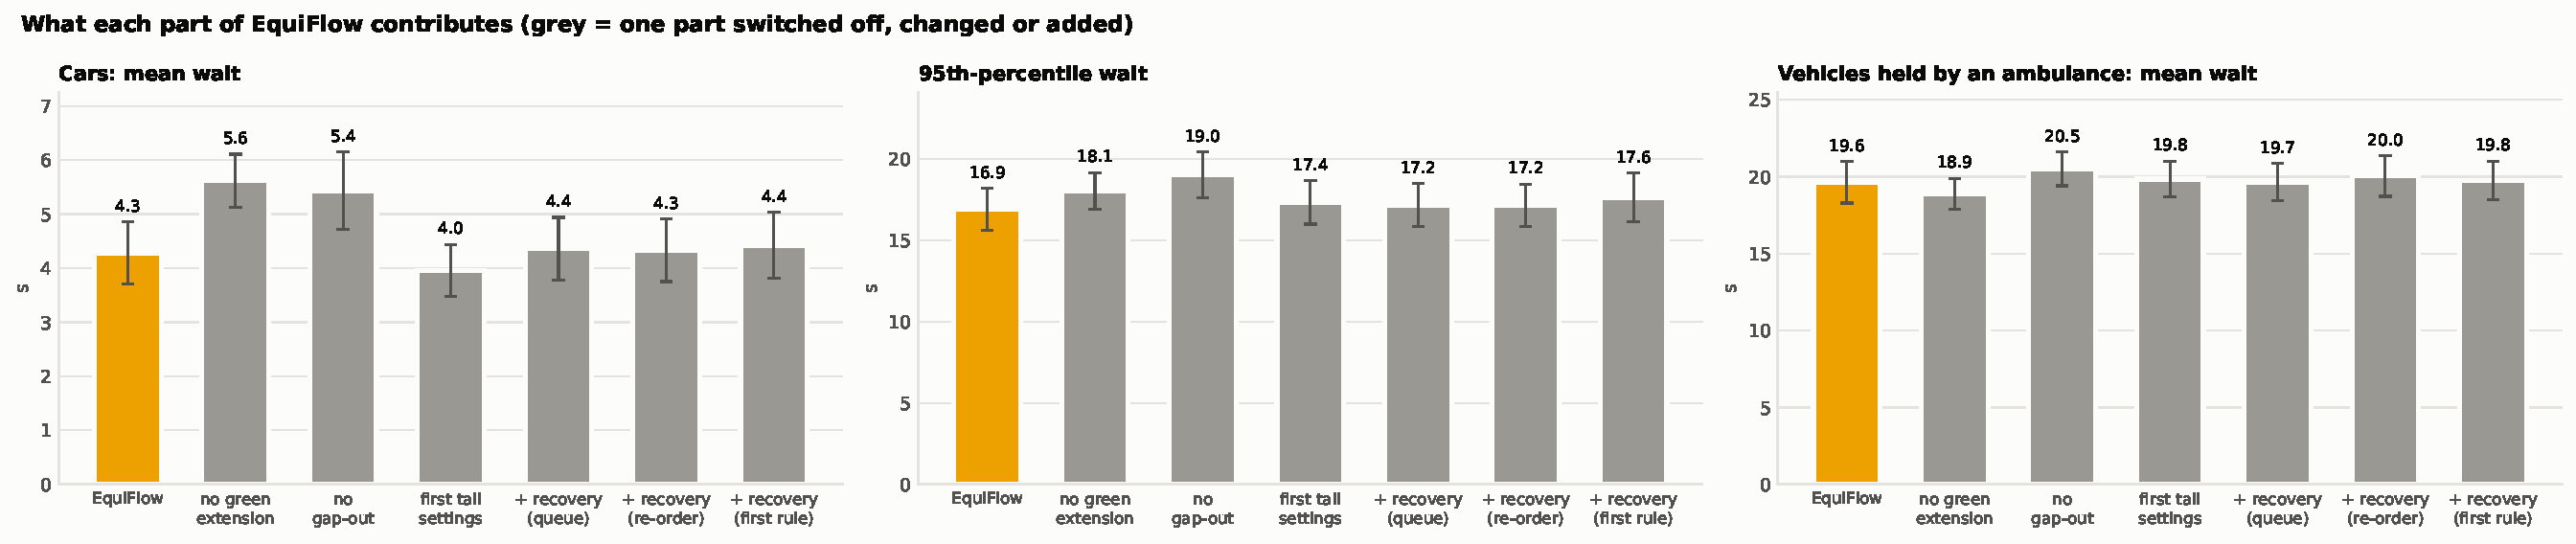
\includegraphics[width=\textwidth]{figures/fig_ablation.pdf}
\caption{Ablations: EquiFlow with one component switched off or replaced.}
\label{fig:it2-ablation}
\end{figure}

Table~\ref{tab:it2-ablation} and Figure~\ref{fig:it2-ablation} switch one component off, change it, or add an
optional one back. \emph{Green extension} gives the largest gain in average waits: without it car wait rises by
1.33\,s (better with it in 95\% of paired runs) and the 95th-percentile wait by 1.16\,s, with no significant
change in the longest wait. In the first evaluation round extension cost 6.6\,s on the longest wait; the tighter
30\,s wait cap and the higher waiting-time weight removed that cost (the first settings have a 4.4\,s longer
longest wait), at 0.3\,s of car wait. \emph{Gap-out} improves every measure: without it car wait rises by 1.15\,s
and the 95th-percentile wait by 2.11\,s (better in 99\% of runs).

\emph{Fair recovery} gives no benefit with any of the three rules. Adding the queue-sized rule raises car wait
by 0.08\,s and the 95th-percentile wait by 0.26\,s; the re-order-only rule changes nothing significantly except a
0.25\,s higher 95th-percentile wait; the first rule is worst (95th percentile +0.74\,s, longest wait +2.2\,s). The
stress scenario (about 40 ambulances per hour, 30 runs per controller) gives the same answer: the queue-sized rule
raises the 95th-percentile wait by 1.3\,s, the first rule by 4.0\,s, and the re-order rule by nothing measurable.
Re-ordering removes the harm but adds no benefit: an adaptive controller that already serves the
longest-waiting busy approach next leaves nothing for a separate recovery phase to fix. Recovery is therefore off
by default.

On the two multi-junction networks (Table~\ref{tab:it2-corridor}) the \emph{green corridor} turns downstream
signals green a little earlier but does not change ambulance travel time, while the vehicles it holds wait
longer: 2.4\,s with the just-in-time rule and 6.8\,s with the first rule. With junctions 300\,m apart, local
priority alone is fast enough, so the corridor is off by default.

\subsection{MARL controller}
\begin{figure}[htbp]
\centering
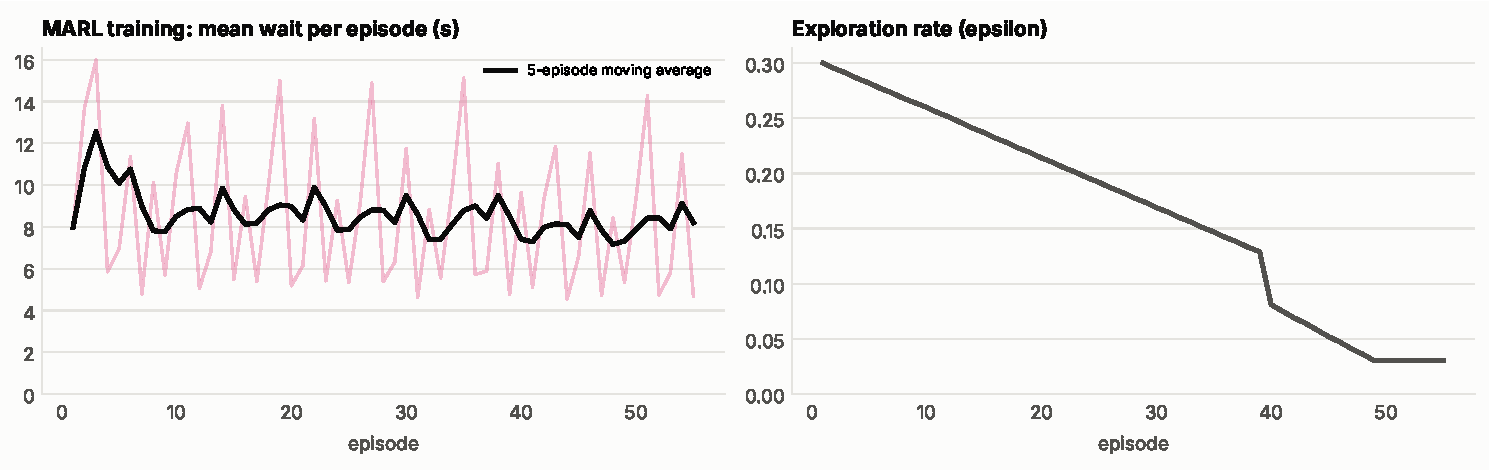
\includegraphics[width=\textwidth]{figures/fig_marl_training.pdf}
\caption{MARL training: mean wait per episode (episodes rotate between networks) and exploration rate.}
\label{fig:it2-marl}
\end{figure}

The first MARL policy (55 training episodes) tied the adaptive heuristic on car wait but had a 1.85\,s higher
95th-percentile wait. Its reward was therefore extended to charge every halted vehicle that has already waited
more than 20\,s (about the 95th-percentile wait), and it was retrained from scratch for 120 episodes on seeds
1--5 with the final junction settings. On the held-out seeds it now beats the heuristic on car wait
($-0.23 \pm 0.18$\,s), but the heuristic's own tail tuning moved further, so MARL's 95th-percentile wait is
$1.43 \pm 0.55$\,s higher and its longest wait 2.9\,s higher, with the same picture on network/demand combinations
it was trained on and on unseen ones (Table~\ref{tab:it2-marl}). The adaptive controller stays the default.

\subsection{Robustness to camera errors}
\begin{figure}[htbp]
\centering
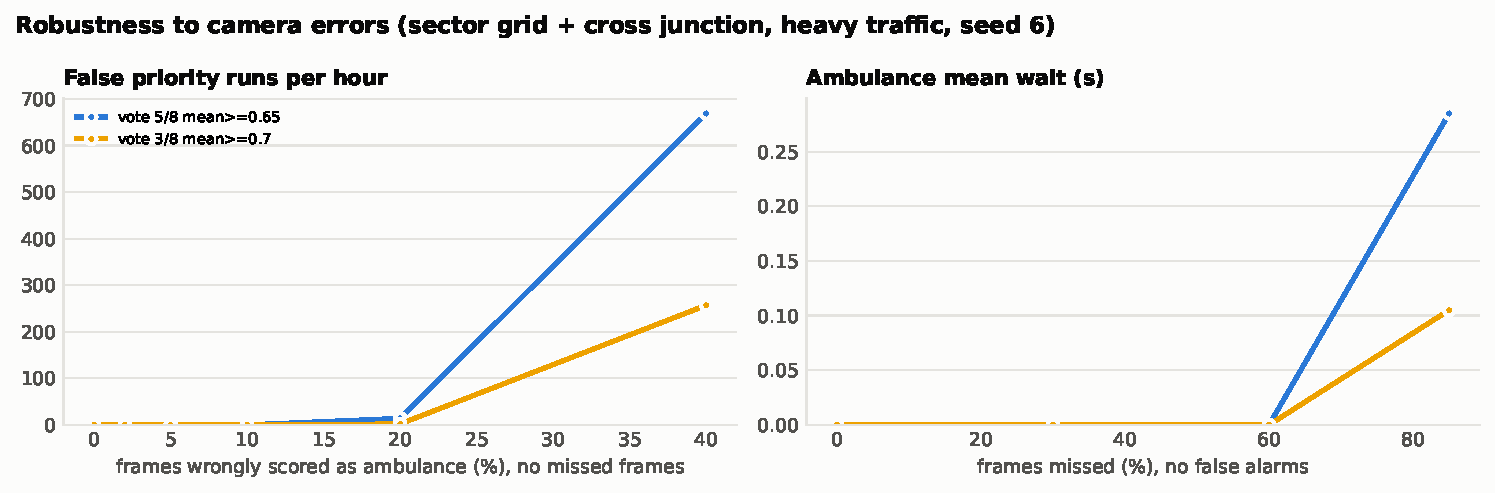
\includegraphics[width=\textwidth]{figures/fig_robustness.pdf}
\caption{False priority runs and ambulance wait as the virtual camera misses frames or scores ordinary
vehicles as ambulances, for the 5-of-8 vote and the live 3-of-8 vote (heavy demand, seed 6).}
\label{fig:it2-robust}
\end{figure}

The sweep was run for both votes (Figure~\ref{fig:it2-robust}). With up to 10\% of frames wrongly scored as
ambulance, neither produces any false priority. At 20\% the 5-of-8 vote (mean $\geq$ 0.65) produces 8--20 false
priority runs per hour and the live 3-of-8 vote (mean $\geq$ 0.70) only 0--4; at 40\% they produce 386--952
and 145--369. The live vote is therefore more tolerant of noisy frames, not less: its stricter mean-score
threshold matters more than the lower vote count. Missing even 85\% of frames barely matters (ambulance wait at
most 0.6\,s). The classifier's per-crop false-alarm rate is 0.9\% on the test split, well inside this margin.

\subsection{Ambulance classifier}
\label{sec:it2-classifier}
\paragraph{Dataset check.} \texttt{Projects/make\_split\_manifest.py} lists all 32\,593 crops with a SHA-1 and a
perceptual hash and looks for images shared between splits. The test split contains no exact copy of a training
image; 134 test crops (3.6\%) are near duplicates of a training crop, all with the same label. The check found
four validation crops labelled ambulance that were copies of training crops labelled other vehicle, and 35
duplicate files inside the training split; all 39 were removed. Removing the four mislabelled copies alone raised
the mid-report model's validation recall from 91.0\% to 91.8\%: all four had been counted as missed ambulances.

\paragraph{Retraining.} Three changes proposed in the mid-report were trained one at a time on the cleaned data and
compared on the validation split only (Table~\ref{tab:it2-cls-val}). Retraining with unchanged settings changes
little; doubling the ambulance crops gives the highest recall but more false alarms; a 128\,px input
(cls\_v5\_img128) is best on PR-AUC and F1 and was selected.

\paragraph{Test split.} Only the selected model and the mid-report model were then run on the held-out test split,
once (Table~\ref{tab:it2-cls-test}). cls\_v5\_img128 is better on every metric: 93.5\% recall at 96.5\% precision
and a 0.9\% false-alarm rate. Recall is lowest on the Pakistani ambulance crops (88.1\%, against 95.9\% on the
public dataset). A threshold chosen on the validation split for 95\% recall gives 95.7\% test recall for the
mid-report model, at 87.7\% precision.

\paragraph{Latency.} On an RTX 4050 laptop GPU the vehicle detector takes 27.7\,ms per 1280\,px frame and the
classifier 1.7\,ms per crop in a batch (Table~\ref{tab:it2-latency}): about 45\,ms per frame, or 22 frames per
second, with ten vehicles in view. Measured back to back, the 128\,px classifier costs the same as the 96\,px one.

\subsection{Tracking on real video}
\label{sec:it2-tracking}
With the new classifier and the old vote (5 of 8, mean $\geq$ 0.65) the pipeline confirmed 5 of the 7 labelled
ambulance passes. \texttt{Projects/tune\_tracking.py} records every track's score per frame once and replays the
vote offline; at the old setting the replay reproduces the pipeline's confirmations exactly on all 12 videos.
Of 360 settings (Table~\ref{tab:it2-tune}), the number of votes K decides the result: every setting with K = 3
and a mean score of 0.70--0.75 confirms all 7 passes with 6 false events, whatever the frame threshold, while
K = 4 or 5 confirm 5. The chosen setting keeps the frame threshold at 0.6 and uses K = 3, mean $\geq$ 0.70.

Table~\ref{tab:it2-tracking} gives the re-run pipeline on all 12 available clips (a thirteenth clip has no source
video): 7 of 7 passes confirmed, on average 0.94\,s after the labelled start, with 6 false confirmations: 3 in
test5, a clip checked to contain no ambulance (a look-alike vehicle), 2 in test12 1.4\,s before a labelled pass,
and 1 in test4. Because the same videos chose and scored the setting, this is optimistic. Choosing the setting on
11 videos and scoring the twelfth, for each video in turn, gives 7 of 7 passes and 11 false events. Seven passes
are far too few for a reliable recall estimate.

\subsection{Performance}
A controller tick takes about 1\,$\mu$s and a MARL decision about 24\,$\mu$s (p99 62\,$\mu$s), against a
100\,000\,$\mu$s tick period (Table~\ref{tab:it2-perf}). A one-hour SUMO run takes about 3\,s.

\section{Failure Analysis}
\begin{table}[htbp]
\centering
\small
\caption{Failure cases found in Iteration 2 and the planned response.}
\label{tab:it2-failures}
\resizebox{\textwidth}{!}{%
\begin{tabular}{lll}
\hline
Failure & Likely cause & Response \\
\hline
Short ambulance tracks missed with a 5-of-8 vote (test12) & too few confident frames before it leaves & resolved: K = 3, re-tuned \\
3 false confirmations in test5 (no ambulance) & ambulance-like vehicle not in training & add its crops as hard negatives \\
Early confirmations (test12, 1.4\,s before the label) & hand-labelled windows are approximate & label from the first visible frame \\
Recall 88\% on Pakistani ambulances (test) & few local ambulance crops in training & collect more local ambulance crops \\
Mislabelled duplicate crops (4 in validation) & copies made while sorting crops & resolved: split manifest + duplicate check \\
False priority at $\geq$20\% per-frame false alarms & vote too permissive for very noisy input & keep per-frame FP $\ll$ 20\%; live 3-of-8 vote is 4$\times$ more tolerant \\
Higher p95 wait than actuated under heavy demand & green length fixed at its start & resolved: extension + tail tuning (gap +0.3\,s, n.s.) \\
Green extension lengthened the longest wait (+6.6\,s) & others held up to the 40\,s cap & resolved: 30\,s cap, wait weight 0.3 \\
Corridor gives no measurable ambulance benefit & junctions 300\,m apart & off by default; just-in-time rule kept as an option \\
Fair recovery gives no benefit (harmful when frequent) & adaptive order already serves delayed approaches & off by default; re-order rule removes the harm \\
MARL better on car wait, worse on tail waits & heuristic tail tuning moved further & longer training, tail-weighted reward \\
\hline
\end{tabular}}
\end{table}

\section{Limitations}
All control results are from simulation; the SUMO cameras are virtual (exact ambulance positions with
simulated classifier scores), so the real camera pipeline and the SUMO evaluation share the controller and the
voting rule but not the video. The live vote (3 of 8) was tuned on the same 12 clips it is scored on, which
hold only 7 ambulance passes. The fair-recovery stress scenario is one synthetic demand pattern. Authentication
is off by default and must be enabled for any deployment.

\section{Iteration Outcome}
The exit criterion is met: the scripted scenario (\texttt{scripts/scripted\_scenario.py}) sends one ambulance,
then two simultaneous ambulances; each is confirmed by detection, receives a protected green, and is followed
by recovery greens, and the whole sequence is recorded in the event log. All 45 automated tests pass. The classifier
was evaluated on the held-out test split and replaced by a better retrained model, all available videos were
processed, and the improvements the first evaluation pointed to were implemented and evaluated on the held-out
seeds: green extension and tail tuning (which closed the heavy-demand gap to actuated control), an approach-level
fairness measure, a re-order-only recovery rule and a recovery stress test, a just-in-time corridor, a retrained
MARL policy and the camera-error sweep for the live vote. Fair recovery and the corridor did not help and are off
by default. The main open items for FYP-2 are reducing the delay of the vehicles an ambulance holds (the cost of
priority that remains), MARL training that also wins on tail waits, more labelled real video, and hard negatives
for ambulance look-alikes.
 after chapter6_iteration1.
% Needs \usepackage{graphicx} (loaded by most report classes).
% All numbers come from sumo/results/heldout/*.csv and the Projects/ evaluation outputs (see docs/RESULTS.md);
% the tables are generated by sumo/latex_tables.py and should be regenerated rather than edited.

\chapter{Iteration 2: Tracking, Control, Integration and Evaluation}
\label{ch:iteration2}

\section{Iteration Objectives}
Iteration~2 turns the perception and simulation work of Iteration~1 into a working, measured system.
Its objectives, taken from the iteration plan, were to:
(i) track ambulances across frames so that a single confident frame cannot trigger priority;
(ii) give a confirmed ambulance a protected green through safe yellow and all-red transitions, also across
neighbouring junctions (green corridor);
(iii) restore service to delayed approaches afterwards (fair recovery) and add a fairness-aware MARL base
controller;
(iv) integrate the modules behind FastAPI and MQTT with a live dashboard; and
(v) evaluate the controllers on repeatable SUMO runs against fixed-time and actuated baselines.
The exit criterion was that a scripted ambulance scenario triggers and completes a logged preemption with
recovery.

\section{Selected Use Cases / Features}
UC-01 (detect an approaching ambulance), UC-02 (estimate traffic state), UC-03 (grant emergency priority),
UC-04 (recover fairly after priority), UC-05 (run a baseline comparison) and UC-06 (monitor the junction on
the dashboard). Requirement coverage after this iteration is summarised in Table~\ref{tab:it2-req}.

\begin{table}[htbp]
\centering
\small
\caption{Functional requirements and test cases addressed in Iteration 2.}
\label{tab:it2-req}
\resizebox{\textwidth}{!}{%
\begin{tabular}{lll}
\hline
Requirement / test & Implementation & Evidence \\
\hline
FR-01--03 detection input, output, logging & \texttt{vision/live.py}, \texttt{eventlog.py} & \texttt{test\_live\_pipeline.py}, CSV event log \\
FR-04 traffic state & SUMO queues; camera approach zones (\texttt{zones:}) & \texttt{test\_fr04\_zone\_...} \\
FR-05 / TC-03 stale detections & 2\,s age limit on external events, K-of-M vote, 60\,s fail-safe & \texttt{test\_tc03\_...} \\
FR-06--08 phases, timing, priority & \texttt{controllers/intersection.py} & \texttt{test\_controller.py} (randomised safety) \\
FR-07 / TC-04 early end of empty green & gap-out after 5\,s, only if another approach has demand & \texttt{test\_tc04\_...} \\
FR-09 / TC-06 logged preemption and recovery & event log + episode table & \texttt{scripts/scripted\_scenario.py} \\
FR-10 recovery uses queue and wait & queue-sized recovery greens, longest wait first & \texttt{test\_fr10\_...} \\
FR-11 baselines & fixed-time, actuated, fixed-time + priority & Section~\ref{sec:it2-results} \\
FR-12 export metrics and configuration & \texttt{run\_manifest.csv} (config + versions per run) & \texttt{results/heldout/} \\
TC-10 repeatability & same seed and configuration give identical results & \texttt{test\_tc10\_...} \\
\hline
\end{tabular}}
\end{table}

\section{Design}
The controller is split into a \emph{base controller} that chooses the next green in normal operation
(fixed-time, adaptive, or the MARL policy) and an \emph{intersection controller} that wraps it with
everything that must never be learned: ambulance priority, minimum green, yellow and all-red, the 90\,s
maximum-wait guard, gap-out and fair recovery. The intersection controller never reads a clock; it is
given the time on every tick, so the same code runs in the live backend (every 0.1\,s) and inside each SUMO
step. Every decision is published as an event on a bus that feeds the REST/WebSocket API, the optional MQTT
bridge and a CSV event log.

\section{Implementation}
\begin{itemize}
\item \textbf{Perception} (\texttt{backend/app/vision/live.py}): YOLO26s vehicle detection with ByteTrack,
the ambulance classifier on each tracked crop (cls\_v5\_img128, retrained in this iteration at 128\,px), and a
confirmation vote over the last 8 frames. The live camera configuration needs 3 ambulance votes (frame score
$\geq$ 0.6) and a mean score of at least 0.70, re-tuned for the new classifier
(Section~\ref{sec:it2-tracking}); the SUMO evaluation and the backend default use 5 of 8 with mean
$\geq$ 0.65. Optional per-approach polygons restrict counting to the lanes that queue for the signal and
report stationary vehicles as the queue.
\item \textbf{Signal control} (\texttt{backend/app/controllers/}): base controllers, the MARL policy
(shared Q-network over per-phase features, pure NumPy) and the intersection controller described above.
\item \textbf{Integration} (\texttt{backend/app/}): FastAPI REST + WebSocket + MJPEG, MQTT topics, a live
SUMO view driven through TraCI, an optional API key on every write endpoint, and the CSV event log.
\item \textbf{Evaluation} (\texttt{sumo/}): \texttt{run\_matrix.py} runs every controller on the same
networks, demand levels and seeds in parallel; \texttt{aggregate.py} computes means, confidence intervals and
paired differences; \texttt{make\_plots.py} and \texttt{latex\_tables.py} produce the figures and tables in
this chapter.
\end{itemize}

\section{Algorithms and Technical Decisions}
\paragraph{Gap-out.} A green that has run at least 5\,s ends early when no vehicle is within 120\,m of its
stop line and another approach has demand. It is never applied during priority and always passes through
the full yellow and all-red.
\paragraph{Green extension.} Actuated control lengthens a green vehicle by vehicle, while the adaptive controller
fixes each green's length when it starts. A base-controller green that reaches its planned length therefore keeps
going while its approach is still at least as busy as every other one, up to 45\,s, and only while no other
approach with a queue has waited 30\,s. To keep the tail of the waiting-time distribution short, the adaptive
controller also weights waiting time more when it chooses the next green (weight 0.3 instead of 0.1). It is never applied during priority or recovery, and every green still
ends through the full yellow and all-red. The two limits were chosen on tuning seeds 1--2, not on the held-out
seeds.
\paragraph{Priority.} After the vote confirms an ambulance, the current green finishes its minimum time,
then yellow and all-red, and the ambulance's approach turns green alone. Priority ends 4\,s after the
ambulance was last seen, or after 60\,s as a fail-safe. Two ambulances are served first come, first served.
\paragraph{Fair recovery.} After priority, the approaches that were held red and have a queue are served in
order of longest wait, each for about as long as its queue needs to clear (2\,s per queued vehicle, at least
5\,s, at most 30\,s). A first version gave every delayed approach a fixed 15\,s green plus extra, and a third
rule only re-orders the delayed approaches and leaves each green's length to the base controller. Because none of
them improved on having no recovery (Section~\ref{sec:it2-ablation}), recovery is off by default and kept as an
option; the scripted exit scenario switches it on to verify the logged recovery sequence.
\paragraph{Green corridor.} Once a camera confirms an ambulance, signals further along its route are asked for
priority \emph{just in time}: only when the ambulance's arrival time is within the time that signal needs to
switch to it (minimum green, yellow and all-red) plus 3\,s, or, if its phase is already green, when that green
would otherwise end just before the ambulance arrives. The first version cleared every signal within 25\,s of
arrival. Neither made ambulances faster on the evaluated networks, so the corridor is off by default.
\paragraph{Stale detections.} An externally reported detection older than 2\,s (or more than 2\,s in the
future) is rejected and logged, so a delayed or replayed message cannot request priority.

\section{Evaluation Set-up}
Six signalised Islamabad junction networks were each run at four demand levels for one simulated hour.
Every controller used the same 120 network/demand/seed combinations with seeds 6--10; the MARL policy was
trained on seeds 1--5, so all evaluation runs are held out. Ambulances are confirmed by a virtual camera per
approach using the real voting rule. Results are reported as mean $\pm$ 95\% confidence interval over runs,
and as \emph{paired} differences on identical runs, which removes the large differences between networks.
Besides network-wide waits, an approach-level measure counts the vehicles an ambulance actually holds: ordinary
vehicles stopped at a junction while a real ambulance is within camera range on another of its approaches. It is
ground truth, so it is measured the same way for controllers that give no priority. A stress scenario (heavy
traffic and about 40 ambulances per hour, three times the heavy level) tests fair recovery separately.

% Generated by sumo/latex_tables.py from the CSV results. Do not edit by hand; re-run the script.

\begin{table}[htbp]
\centering
\small
\caption{Held-out evaluation: mean $\pm$ 95\% confidence interval over one-hour SUMO runs (seeds 6--10).}
\label{tab:it2-main}
\resizebox{\textwidth}{!}{%
\begin{tabular}{lccccc}
\hline
Metric & Fixed-time & Actuated & Fixed + priority & EquiFlow & EquiFlow (MARL) \\
\hline
Car mean wait (s) & 16.87 $\pm$ 1.02 & 6.28 $\pm$ 1.01 & 10.36 $\pm$ 0.86 & 4.28 $\pm$ 0.57 & 4.05 $\pm$ 0.53 \\
Ordinary vehicles, mean wait (s) & 17.07 $\pm$ 1.05 & 6.23 $\pm$ 0.99 & 10.29 $\pm$ 0.84 & 4.32 $\pm$ 0.56 & 4.10 $\pm$ 0.52 \\
95th-percentile wait (s) & 51.71 $\pm$ 1.61 & 17.87 $\pm$ 2.13 & 29.44 $\pm$ 1.69 & 16.91 $\pm$ 1.31 & 18.34 $\pm$ 1.65 \\
Longest single wait (s) & 72.17 $\pm$ 3.72 & 36.71 $\pm$ 4.45 & 57.69 $\pm$ 5.03 & 39.84 $\pm$ 3.34 & 42.69 $\pm$ 3.72 \\
Share waiting $>$60 s & 0.030 $\pm$ 0.005 & 0.002 $\pm$ 0.001 & 0.002 $\pm$ 0.001 & 0.001 $\pm$ 0.000 & 0.001 $\pm$ 0.001 \\
Worst approach, mean wait (s) & 21.98 $\pm$ 1.37 & 7.95 $\pm$ 1.10 & 13.40 $\pm$ 1.01 & 5.63 $\pm$ 0.59 & 5.49 $\pm$ 0.58 \\
Jain index across approaches & 0.915 $\pm$ 0.025 & 0.888 $\pm$ 0.025 & 0.904 $\pm$ 0.025 & 0.878 $\pm$ 0.030 & 0.879 $\pm$ 0.029 \\
Held by an ambulance, mean wait (s) & 36.17 $\pm$ 1.16 & 12.39 $\pm$ 1.37 & 25.22 $\pm$ 1.63 & 19.64 $\pm$ 1.35 & 19.55 $\pm$ 1.43 \\
Held by an ambulance, p95 wait (s) & 56.02 $\pm$ 2.19 & 22.53 $\pm$ 3.00 & 39.74 $\pm$ 3.26 & 29.47 $\pm$ 2.18 & 31.80 $\pm$ 3.17 \\
Ambulance mean wait (s) & 13.75 $\pm$ 1.16 & 7.42 $\pm$ 1.31 & 0.19 $\pm$ 0.08 & 0.10 $\pm$ 0.06 & 0.10 $\pm$ 0.05 \\
Ambulance travel time (s) & 59.14 $\pm$ 2.42 & 52.75 $\pm$ 2.40 & 43.19 $\pm$ 2.21 & 42.68 $\pm$ 2.22 & 42.54 $\pm$ 2.22 \\
Detection to green (s) & -- & -- & 2.57 $\pm$ 0.17 & 2.37 $\pm$ 0.13 & 2.39 $\pm$ 0.16 \\
Recovery interval (s) & -- & -- & 0.00 $\pm$ 0.00 & 0.00 $\pm$ 0.00 & 0.00 $\pm$ 0.00 \\
Runs & 120 & 120 & 120 & 120 & 120 \\
\hline
\end{tabular}}
\end{table}

\begin{table}[htbp]
\centering
\small
\caption{Ablations: EquiFlow with one component switched off, changed or added (all networks).}
\label{tab:it2-ablation}
\resizebox{\textwidth}{!}{%
\begin{tabular}{lccccccc}
\hline
Metric & EquiFlow & No extension & No gap-out & First tail settings & + Recovery (queue) & + Recovery (re-order) & + Recovery (first rule) \\
\hline
Car mean wait (s) & 4.28 $\pm$ 0.57 & 5.62 $\pm$ 0.49 & 5.43 $\pm$ 0.71 & 3.96 $\pm$ 0.48 & 4.36 $\pm$ 0.58 & 4.33 $\pm$ 0.58 & 4.42 $\pm$ 0.61 \\
95th-percentile wait (s) & 16.91 $\pm$ 1.31 & 18.07 $\pm$ 1.12 & 19.02 $\pm$ 1.41 & 17.35 $\pm$ 1.34 & 17.17 $\pm$ 1.32 & 17.16 $\pm$ 1.31 & 17.65 $\pm$ 1.49 \\
Longest single wait (s) & 39.84 $\pm$ 3.34 & 38.48 $\pm$ 3.82 & 42.21 $\pm$ 3.22 & 44.19 $\pm$ 3.08 & 39.78 $\pm$ 3.32 & 40.31 $\pm$ 3.60 & 41.99 $\pm$ 3.90 \\
Jain index across approaches & 0.878 $\pm$ 0.030 & 0.911 $\pm$ 0.025 & 0.889 $\pm$ 0.029 & 0.864 $\pm$ 0.032 & 0.881 $\pm$ 0.030 & 0.880 $\pm$ 0.030 & 0.877 $\pm$ 0.030 \\
Held by an ambulance, mean wait (s) & 19.64 $\pm$ 1.35 & 18.89 $\pm$ 1.00 & 20.50 $\pm$ 1.09 & 19.84 $\pm$ 1.17 & 19.66 $\pm$ 1.21 & 20.04 $\pm$ 1.32 & 19.77 $\pm$ 1.24 \\
Ambulance mean wait (s) & 0.10 $\pm$ 0.06 & 0.13 $\pm$ 0.06 & 0.14 $\pm$ 0.08 & 0.10 $\pm$ 0.04 & 0.10 $\pm$ 0.05 & 0.10 $\pm$ 0.06 & 0.08 $\pm$ 0.03 \\
Ambulance travel time (s) & 42.68 $\pm$ 2.22 & 42.92 $\pm$ 2.22 & 42.82 $\pm$ 2.22 & 42.57 $\pm$ 2.22 & 42.65 $\pm$ 2.22 & 42.66 $\pm$ 2.22 & 42.63 $\pm$ 2.21 \\
Recovery interval (s) & 0.00 $\pm$ 0.00 & 0.00 $\pm$ 0.00 & 0.00 $\pm$ 0.00 & 0.00 $\pm$ 0.00 & 22.94 $\pm$ 0.94 & 21.61 $\pm$ 0.88 & 28.25 $\pm$ 1.35 \\
Runs & 120 & 120 & 120 & 120 & 120 & 120 & 120 \\
\hline
\end{tabular}}
\end{table}

\begin{table}[htbp]
\centering
\small
\caption{Green corridor on the two multi-junction networks (sector grid, diamond): EquiFlow (no corridor) minus EquiFlow with each corridor rule, on identical runs. Negative = EquiFlow lower. $^*$: the 95\% CI excludes zero.}
\label{tab:it2-corridor}
\begin{tabular}{llccc}
\hline
Versus & Metric & Difference (95\% CI) & EquiFlow better in & Runs \\
\hline
+ Corridor (just in time) & Car mean wait (s) & -0.06 $\pm$ 0.07 & 40\% & 40 \\
+ Corridor (just in time) & 95th-percentile wait (s) & -0.37 $\pm$ 0.32$^*$ & 32\% & 40 \\
+ Corridor (just in time) & Longest single wait (s) & -0.17 $\pm$ 1.30 & 22\% & 40 \\
+ Corridor (just in time) & Held by an ambulance, mean wait (s) & -2.43 $\pm$ 1.31$^*$ & 63\% & 35 \\
+ Corridor (just in time) & Ambulance mean wait (s) & -0.02 $\pm$ 0.03 & 8\% & 40 \\
+ Corridor (just in time) & Ambulance travel time (s) & +0.04 $\pm$ 0.12 & 18\% & 40 \\
+ Corridor (25 s ETA) & Car mean wait (s) & -0.06 $\pm$ 0.07 & 55\% & 40 \\
+ Corridor (25 s ETA) & 95th-percentile wait (s) & -0.71 $\pm$ 0.47$^*$ & 52\% & 40 \\
+ Corridor (25 s ETA) & Longest single wait (s) & -4.33 $\pm$ 2.17$^*$ & 60\% & 40 \\
+ Corridor (25 s ETA) & Held by an ambulance, mean wait (s) & -6.76 $\pm$ 1.92$^*$ & 91\% & 35 \\
+ Corridor (25 s ETA) & Ambulance mean wait (s) & -0.01 $\pm$ 0.02 & 2\% & 40 \\
+ Corridor (25 s ETA) & Ambulance travel time (s) & +0.08 $\pm$ 0.11 & 20\% & 40 \\
\hline
\end{tabular}
\end{table}

\begin{table}[htbp]
\centering
\small
\caption{Paired comparison on identical runs (same network, demand and seed): EquiFlow minus the other controller. Negative values mean EquiFlow is lower. $^*$: the 95\% CI excludes zero.}
\label{tab:it2-paired}
\begin{tabular}{llccc}
\hline
Versus & Metric & Difference (95\% CI) & EquiFlow better in & Runs \\
\hline
Fixed-time & Car mean wait (s) & -12.59 $\pm$ 0.66$^*$ & 100\% & 120 \\
Fixed-time & 95th-percentile wait (s) & -34.80 $\pm$ 1.19$^*$ & 100\% & 120 \\
Fixed-time & Longest single wait (s) & -32.33 $\pm$ 3.77$^*$ & 97\% & 120 \\
Fixed-time & Ambulance mean wait (s) & -13.64 $\pm$ 1.13$^*$ & 100\% & 120 \\
Actuated & Car mean wait (s) & -2.00 $\pm$ 0.61$^*$ & 68\% & 120 \\
Actuated & 95th-percentile wait (s) & -0.96 $\pm$ 1.32 & 48\% & 120 \\
Actuated & Longest single wait (s) & +3.13 $\pm$ 3.28 & 30\% & 120 \\
Actuated & Ambulance mean wait (s) & -7.32 $\pm$ 1.29$^*$ & 99\% & 120 \\
Fixed + priority & Car mean wait (s) & -6.08 $\pm$ 0.42$^*$ & 100\% & 120 \\
Fixed + priority & 95th-percentile wait (s) & -12.53 $\pm$ 0.82$^*$ & 100\% & 120 \\
Fixed + priority & Longest single wait (s) & -17.85 $\pm$ 3.19$^*$ & 85\% & 120 \\
Fixed + priority & Ambulance mean wait (s) & -0.09 $\pm$ 0.06$^*$ & 28\% & 120 \\
EquiFlow (MARL) & Car mean wait (s) & +0.23 $\pm$ 0.18$^*$ & 48\% & 120 \\
EquiFlow (MARL) & 95th-percentile wait (s) & -1.43 $\pm$ 0.55$^*$ & 60\% & 120 \\
EquiFlow (MARL) & Longest single wait (s) & -2.85 $\pm$ 1.97$^*$ & 62\% & 120 \\
EquiFlow (MARL) & Ambulance mean wait (s) & +0.01 $\pm$ 0.05 & 12\% & 120 \\
No gap-out & Car mean wait (s) & -1.15 $\pm$ 0.18$^*$ & 99\% & 120 \\
No gap-out & 95th-percentile wait (s) & -2.11 $\pm$ 0.27$^*$ & 91\% & 120 \\
No gap-out & Longest single wait (s) & -2.37 $\pm$ 1.94$^*$ & 60\% & 120 \\
No gap-out & Ambulance mean wait (s) & -0.04 $\pm$ 0.05 & 17\% & 120 \\
No extension & Car mean wait (s) & -1.33 $\pm$ 0.18$^*$ & 95\% & 120 \\
No extension & 95th-percentile wait (s) & -1.16 $\pm$ 0.38$^*$ & 59\% & 120 \\
No extension & Longest single wait (s) & +1.36 $\pm$ 2.00 & 32\% & 120 \\
No extension & Ambulance mean wait (s) & -0.03 $\pm$ 0.04 & 21\% & 120 \\
First tail settings & Car mean wait (s) & +0.32 $\pm$ 0.13$^*$ & 34\% & 120 \\
First tail settings & 95th-percentile wait (s) & -0.44 $\pm$ 0.29$^*$ & 41\% & 120 \\
First tail settings & Longest single wait (s) & -4.35 $\pm$ 2.09$^*$ & 62\% & 120 \\
First tail settings & Ambulance mean wait (s) & +0.00 $\pm$ 0.05 & 11\% & 120 \\
+ Recovery (queue) & Car mean wait (s) & -0.08 $\pm$ 0.07$^*$ & 59\% & 120 \\
+ Recovery (queue) & 95th-percentile wait (s) & -0.26 $\pm$ 0.21$^*$ & 46\% & 120 \\
+ Recovery (queue) & Longest single wait (s) & +0.06 $\pm$ 1.72 & 42\% & 120 \\
+ Recovery (queue) & Ambulance mean wait (s) & +0.00 $\pm$ 0.03 & 9\% & 120 \\
+ Recovery (re-order) & Car mean wait (s) & -0.05 $\pm$ 0.06 & 53\% & 120 \\
+ Recovery (re-order) & 95th-percentile wait (s) & -0.25 $\pm$ 0.18$^*$ & 40\% & 120 \\
+ Recovery (re-order) & Longest single wait (s) & -0.47 $\pm$ 1.58 & 33\% & 120 \\
+ Recovery (re-order) & Ambulance mean wait (s) & +0.00 $\pm$ 0.04 & 3\% & 120 \\
+ Recovery (first rule) & Car mean wait (s) & -0.14 $\pm$ 0.09$^*$ & 59\% & 120 \\
+ Recovery (first rule) & 95th-percentile wait (s) & -0.74 $\pm$ 0.34$^*$ & 45\% & 120 \\
+ Recovery (first rule) & Longest single wait (s) & -2.15 $\pm$ 1.81$^*$ & 48\% & 120 \\
+ Recovery (first rule) & Ambulance mean wait (s) & +0.02 $\pm$ 0.05 & 8\% & 120 \\
\hline
\end{tabular}
\end{table}

\begin{table}[htbp]
\centering
\small
\caption{MARL minus adaptive EquiFlow on identical runs, split by whether the network/demand combination was used in MARL training. All seeds are unseen. Negative = MARL lower.}
\label{tab:it2-marl}
\begin{tabular}{lcc}
\hline
Metric & Trained combinations & Unseen combinations \\
\hline
Car mean wait (s) & -0.23 $\pm$ 0.27 (n=40) & -0.23 $\pm$ 0.24 (n=80) \\
95th-percentile wait (s) & +0.84 $\pm$ 0.54 (n=40) & +1.73 $\pm$ 0.77 (n=80) \\
Jain index across approaches & +0.001 $\pm$ 0.011 (n=40) & +0.001 $\pm$ 0.010 (n=80) \\
Ambulance mean wait (s) & +0.00 $\pm$ 0.03 (n=40) & -0.01 $\pm$ 0.07 (n=80) \\
\hline
\end{tabular}
\end{table}

\begin{table}[htbp]
\centering
\small
\caption{Signal controller timing on one CPU core (sumo/benchmark.py). The live backend ticks every 100\,000\,$\mu$s.}
\label{tab:it2-perf}
\begin{tabular}{lcccc}
\hline
Measured & Mean ($\mu$s) & Median & p99 & Max \\
\hline
tick (fixed\_time) & 0.94 & 0.92 & 3.21 & 99.37 \\
decision (fixed\_time) & 0.42 & 0.38 & 0.63 & 467.97 \\
tick (adaptive) & 1.07 & 0.95 & 3.77 & 680.95 \\
decision (adaptive) & 1.39 & 1.2 & 2.68 & 935.52 \\
tick (marl) & 1.35 & 0.94 & 5.07 & 173.0 \\
decision (marl) & 23.83 & 19.82 & 61.69 & 4408.28 \\
\hline
\end{tabular}
\end{table}

\begin{table}[htbp]
\centering
\small
\caption{Tracking pipeline (YOLO26s + ByteTrack + cls\_v5\_img128, 3-of-8 vote with mean score $\geq$ 0.70) on the Islamabad videos. A pass counts as detected if confirmed within 1\,s of its hand-labelled window.}
\label{tab:it2-tracking}
\begin{tabular}{lcccccc}
\hline
Video & Crops used in & Passes & Detected & Missed & False events & Latency (s) \\
\hline
test1 & no & 1 & 1 & 0 & 0 & 0.48 \\
test11 & test & 0 & 0 & 0 & 0 & -- \\
test12 & no & 3 & 3 & 0 & 2 & 2.00 0.00 0.60 \\
test2 & no & 1 & 1 & 0 & 0 & 0.07 \\
test3 & no & 1 & 1 & 0 & 0 & 3.37 \\
test4 & no & 1 & 1 & 0 & 1 & 0.07 \\
test5 & no & 0 & 0 & 0 & 3 & -- \\
test6 & train & 0 & 0 & 0 & 0 & -- \\
test8 & train & 0 & 0 & 0 & 0 & -- \\
test9 & val & 0 & 0 & 0 & 0 & -- \\
v1 & train & 0 & 0 & 0 & 0 & -- \\
v2 & train & 0 & 0 & 0 & 0 & -- \\
\hline
\end{tabular}
\end{table}

\begin{table}[htbp]
\centering
\small
\caption{Ambulance classifier on the held-out test split (Projects/eval\_detector.py, threshold 0.5; 768 ambulance and 2\,953 other-vehicle crops).}
\label{tab:it2-cls-test}
\begin{tabular}{lccccccc}
\hline
Model & Accuracy & Precision & Recall & F1 & False alarms & ROC-AUC & PR-AUC \\
\hline
cls\_v4-2 (mid-report) & 97.7\% & 95.7\% & 92.8\% & 0.942 & 1.1\% & 0.993 & 0.981 \\
cls\_v5\_img128 (pipeline) & 98.0\% & 96.5\% & 93.5\% & 0.950 & 0.9\% & 0.995 & 0.985 \\
\hline
\end{tabular}
\end{table}

\begin{table}[htbp]
\centering
\small
\caption{Classifier training runs on the cleaned validation split (yolo26n-cls, 30 epochs; Projects/train\_cls\_v5.py). The model was chosen here and then run once on the test split.}
\label{tab:it2-cls-val}
\begin{tabular}{llccccc}
\hline
Run & Change & PR-AUC & Recall & Precision & F1 & False alarms \\
\hline
cls\_v4-2 & mid-report model & 0.973 & 91.8\% & 95.6\% & 0.937 & 0.7\% \\
cls\_v5\_base & same settings, cleaned data & 0.975 & 91.8\% & 94.5\% & 0.931 & 0.8\% \\
cls\_v5\_img128 & input 128\,px & 0.979 & 92.8\% & 95.0\% & 0.939 & 0.8\% \\
cls\_v5\_os2 & ambulance crops $\times$2 & 0.975 & 93.7\% & 92.8\% & 0.933 & 1.1\% \\
\hline
\end{tabular}
\end{table}

\begin{table}[htbp]
\centering
\small
\caption{Re-tuning the confirmation vote for cls\_v5\_img128 on the 12 Islamabad videos (Projects/tune\_tracking.py, 360 settings replayed offline; window M = 8 frames).}
\label{tab:it2-tune}
\begin{tabular}{lcccccc}
\hline
Setting & Frame threshold & Mean score & K of 8 & Passes detected & False events & Latency (s) \\
\hline
before & 0.6 & 0.65 & 5 & 5 of 7 & 6 & 0.99 \\
after & 0.6 & 0.7 & 3 & 7 of 7 & 6 & 0.94 \\
\hline
\end{tabular}
\end{table}

\begin{table}[htbp]
\centering
\small
\caption{Perception latency on an RTX 4050 laptop GPU (Projects/eval\_detector.py, a real 1280\,px video frame).}
\label{tab:it2-latency}
\begin{tabular}{lccc}
\hline
Stage & Mean (ms) & Median (ms) & p95 (ms) \\
\hline
YOLO26s vehicle detector, one frame & 27.71 & 26.93 & 32.01 \\
classifier, one crop & 7.94 & 7.53 & 10.65 \\
classifier, batch of 16 crops (1.71\,ms per crop) & 27.4 & 26.78 & 33.74 \\
\hline
full pipeline, 10 vehicles in view (estimate) & 44.8 & & \\
\hline
\end{tabular}
\end{table}



\section{Results}
\label{sec:it2-results}
\begin{figure}[htbp]
\centering
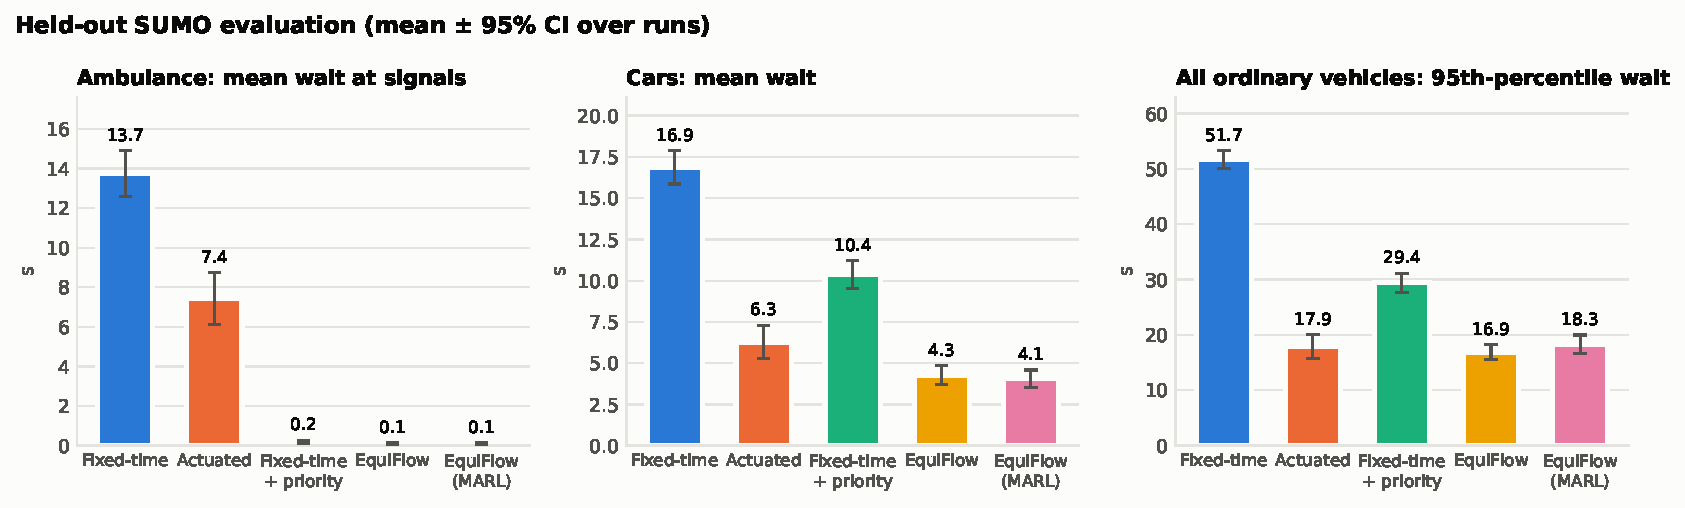
\includegraphics[width=\textwidth]{figures/fig_main_comparison.pdf}
\caption{Held-out evaluation: ambulance wait, car wait and 95th-percentile wait per controller
(mean $\pm$ 95\% CI over 120 runs each).}
\label{fig:it2-main}
\end{figure}

Table~\ref{tab:it2-main} and Figure~\ref{fig:it2-main} give the main comparison. EquiFlow reduces the
ambulance's mean wait at signals from 13.75\,s (fixed-time) and 7.42\,s (actuated) to 0.10\,s, and its travel
time by 16.5\,s (28\%) and 10.1\,s (19\%) respectively. Ordinary traffic also waits less: car wait is 4.28\,s
against 16.87\,s for fixed-time and 6.28\,s for actuated. The paired comparison (Table~\ref{tab:it2-paired})
puts the advantage over actuated at $-2.00 \pm 0.61$\,s (better in 68\% of paired runs), and the worst-served
approach waits 2.3\,s less. The 95th-percentile wait ($-0.96 \pm 1.32$\,s), the longest single wait
($+3.1 \pm 3.3$\,s) and the Jain index across approaches are statistically level with actuated. The price of
priority is paid by the vehicles an ambulance holds: they wait 19.6\,s on average, against 12.4\,s with actuated
control (which never holds them), 25.2\,s with fixed-time plus simple priority and 36.2\,s with fixed-time.

\begin{figure}[htbp]
\centering
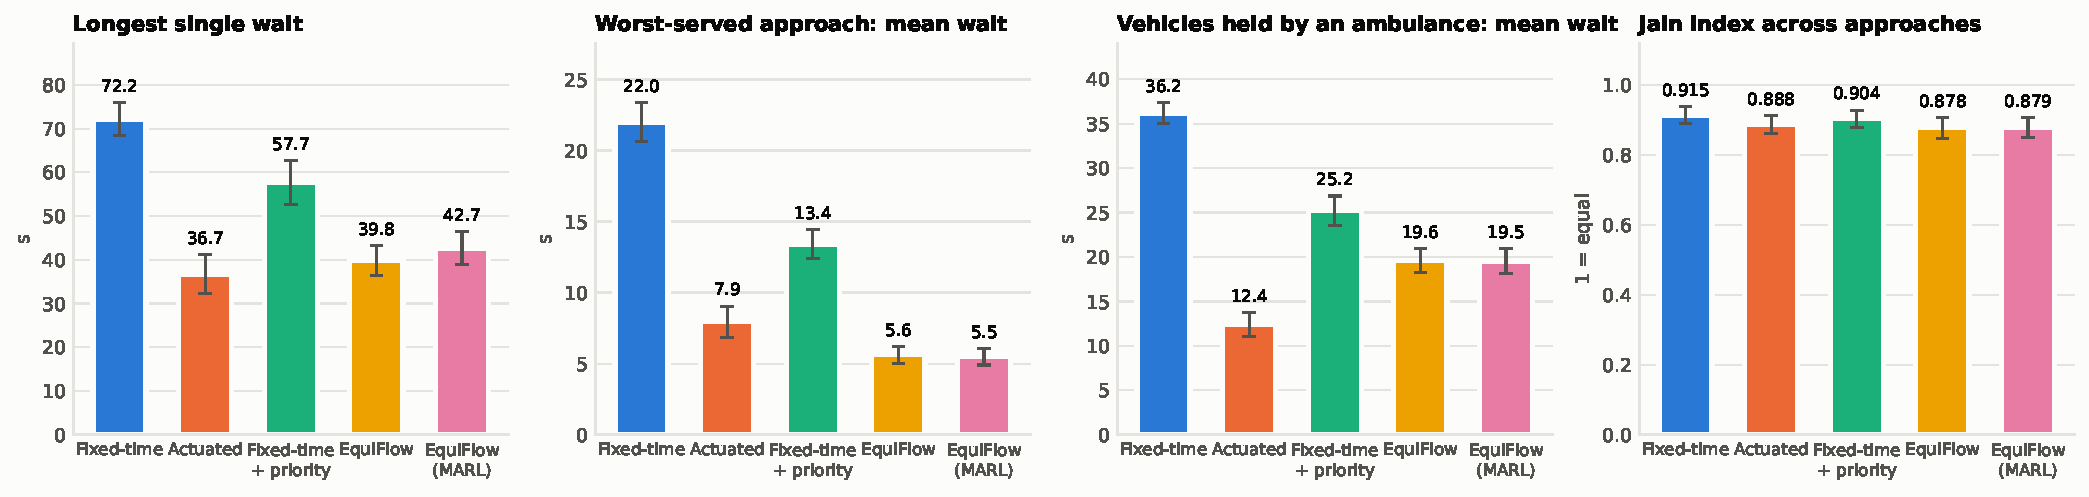
\includegraphics[width=\textwidth]{figures/fig_fairness.pdf}
\caption{Fairness: longest single wait, the worst-served approach's mean wait, the mean wait of the vehicles
held by an ambulance, and Jain's index across approaches.}
\label{fig:it2-fairness}
\end{figure}

\begin{figure}[htbp]
\centering
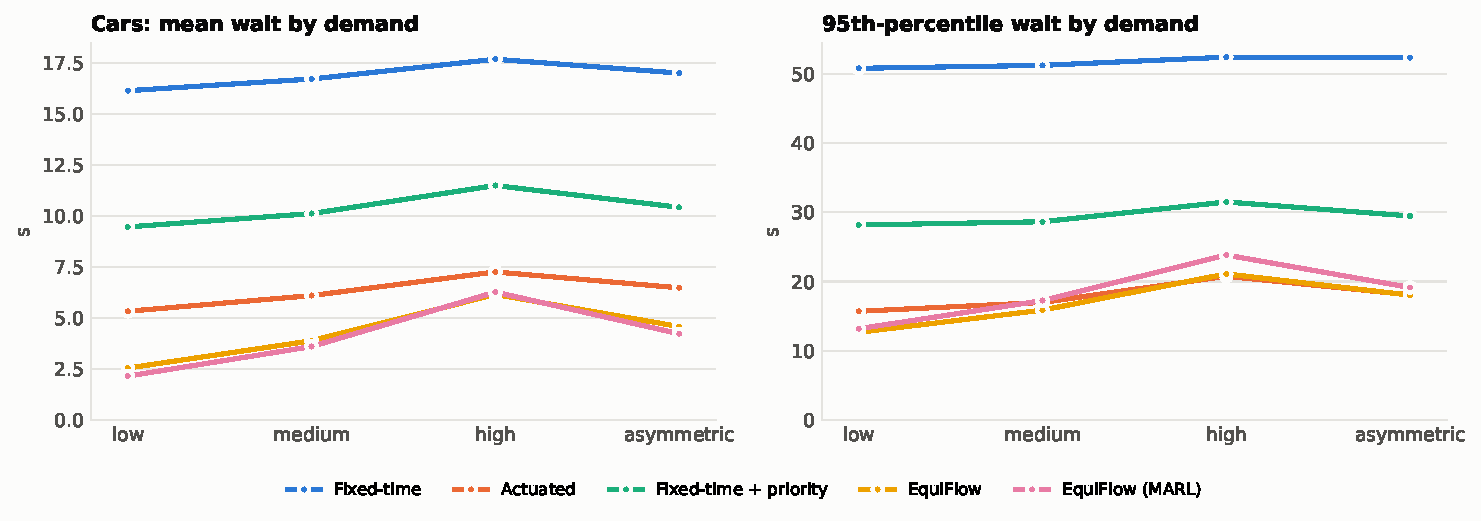
\includegraphics[width=\textwidth]{figures/fig_by_demand.pdf}
\caption{Car mean wait and 95th-percentile wait by demand level.}
\label{fig:it2-demand}
\end{figure}

Under heavy demand (Figure~\ref{fig:it2-demand}) EquiFlow's car wait is below actuated (6.15 against
7.25\,s; 6.92\,s in the first evaluation), and its 95th-percentile wait is now level (21.10 against 20.76\,s, a
paired difference of $+0.33 \pm 2.87$\,s, against $+1.68$\,s in the first evaluation). This is despite every
EquiFlow phase change costing 3\,s of yellow and 2\,s of all-red, against 4\,s of yellow and no all-red in SUMO's
actuated plans; the all-red is kept for safety.

\subsection{Ablations}
\label{sec:it2-ablation}
\begin{figure}[htbp]
\centering
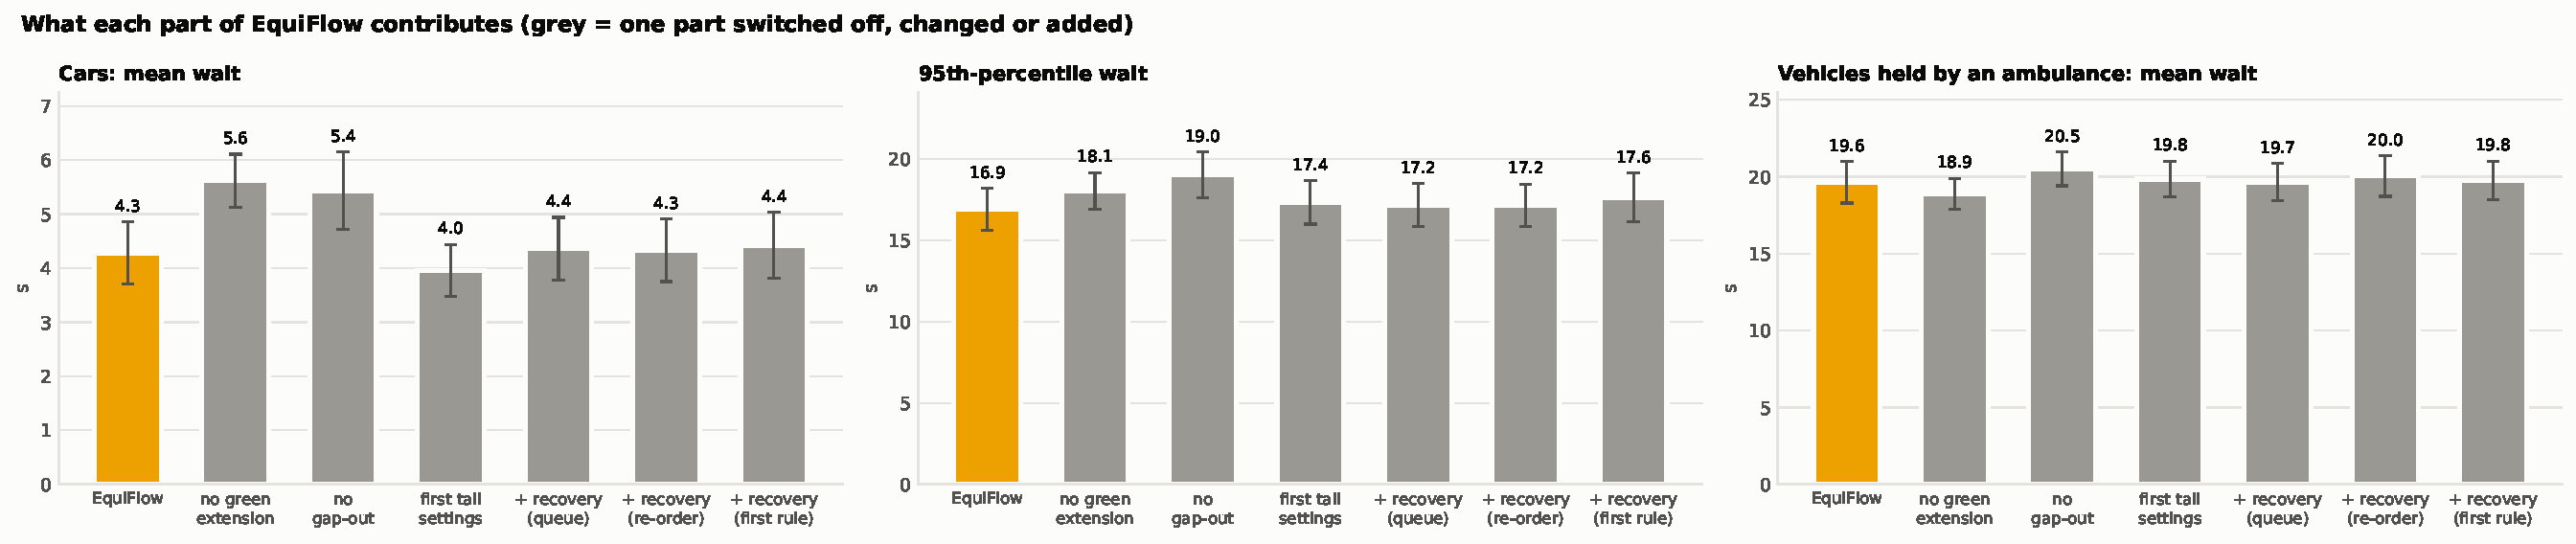
\includegraphics[width=\textwidth]{figures/fig_ablation.pdf}
\caption{Ablations: EquiFlow with one component switched off or replaced.}
\label{fig:it2-ablation}
\end{figure}

Table~\ref{tab:it2-ablation} and Figure~\ref{fig:it2-ablation} switch one component off, change it, or add an
optional one back. \emph{Green extension} gives the largest gain in average waits: without it car wait rises by
1.33\,s (better with it in 95\% of paired runs) and the 95th-percentile wait by 1.16\,s, with no significant
change in the longest wait. In the first evaluation round extension cost 6.6\,s on the longest wait; the tighter
30\,s wait cap and the higher waiting-time weight removed that cost (the first settings have a 4.4\,s longer
longest wait), at 0.3\,s of car wait. \emph{Gap-out} improves every measure: without it car wait rises by 1.15\,s
and the 95th-percentile wait by 2.11\,s (better in 99\% of runs).

\emph{Fair recovery} gives no benefit with any of the three rules. Adding the queue-sized rule raises car wait
by 0.08\,s and the 95th-percentile wait by 0.26\,s; the re-order-only rule changes nothing significantly except a
0.25\,s higher 95th-percentile wait; the first rule is worst (95th percentile +0.74\,s, longest wait +2.2\,s). The
stress scenario (about 40 ambulances per hour, 30 runs per controller) gives the same answer: the queue-sized rule
raises the 95th-percentile wait by 1.3\,s, the first rule by 4.0\,s, and the re-order rule by nothing measurable.
Re-ordering removes the harm but adds no benefit: an adaptive controller that already serves the
longest-waiting busy approach next leaves nothing for a separate recovery phase to fix. Recovery is therefore off
by default.

On the two multi-junction networks (Table~\ref{tab:it2-corridor}) the \emph{green corridor} turns downstream
signals green a little earlier but does not change ambulance travel time, while the vehicles it holds wait
longer: 2.4\,s with the just-in-time rule and 6.8\,s with the first rule. With junctions 300\,m apart, local
priority alone is fast enough, so the corridor is off by default.

\subsection{MARL controller}
\begin{figure}[htbp]
\centering
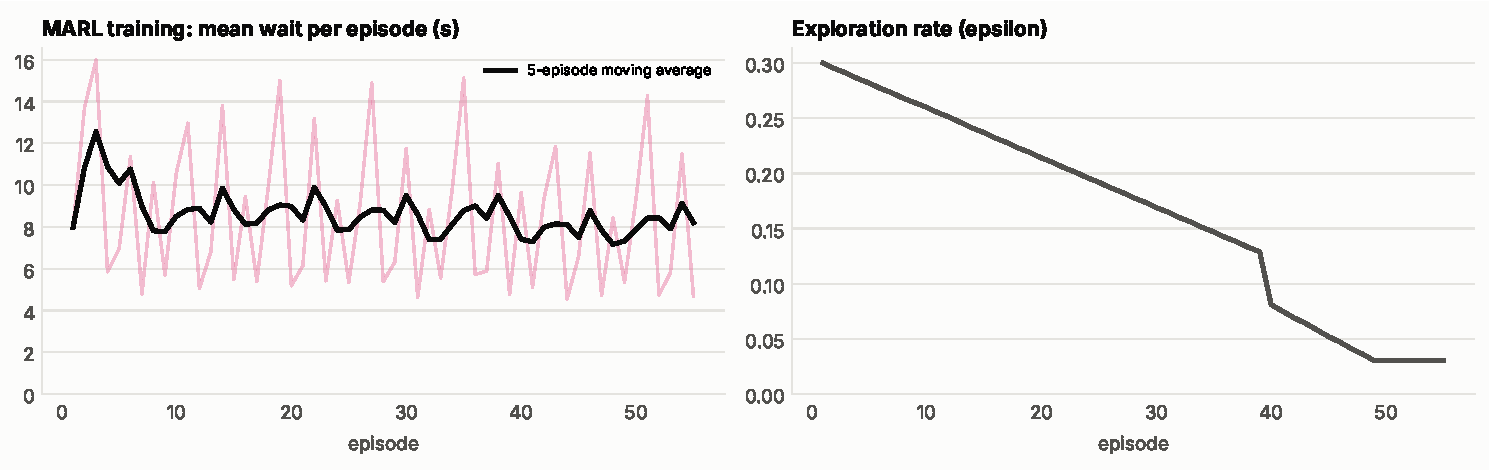
\includegraphics[width=\textwidth]{figures/fig_marl_training.pdf}
\caption{MARL training: mean wait per episode (episodes rotate between networks) and exploration rate.}
\label{fig:it2-marl}
\end{figure}

The first MARL policy (55 training episodes) tied the adaptive heuristic on car wait but had a 1.85\,s higher
95th-percentile wait. Its reward was therefore extended to charge every halted vehicle that has already waited
more than 20\,s (about the 95th-percentile wait), and it was retrained from scratch for 120 episodes on seeds
1--5 with the final junction settings. On the held-out seeds it now beats the heuristic on car wait
($-0.23 \pm 0.18$\,s), but the heuristic's own tail tuning moved further, so MARL's 95th-percentile wait is
$1.43 \pm 0.55$\,s higher and its longest wait 2.9\,s higher, with the same picture on network/demand combinations
it was trained on and on unseen ones (Table~\ref{tab:it2-marl}). The adaptive controller stays the default.

\subsection{Robustness to camera errors}
\begin{figure}[htbp]
\centering
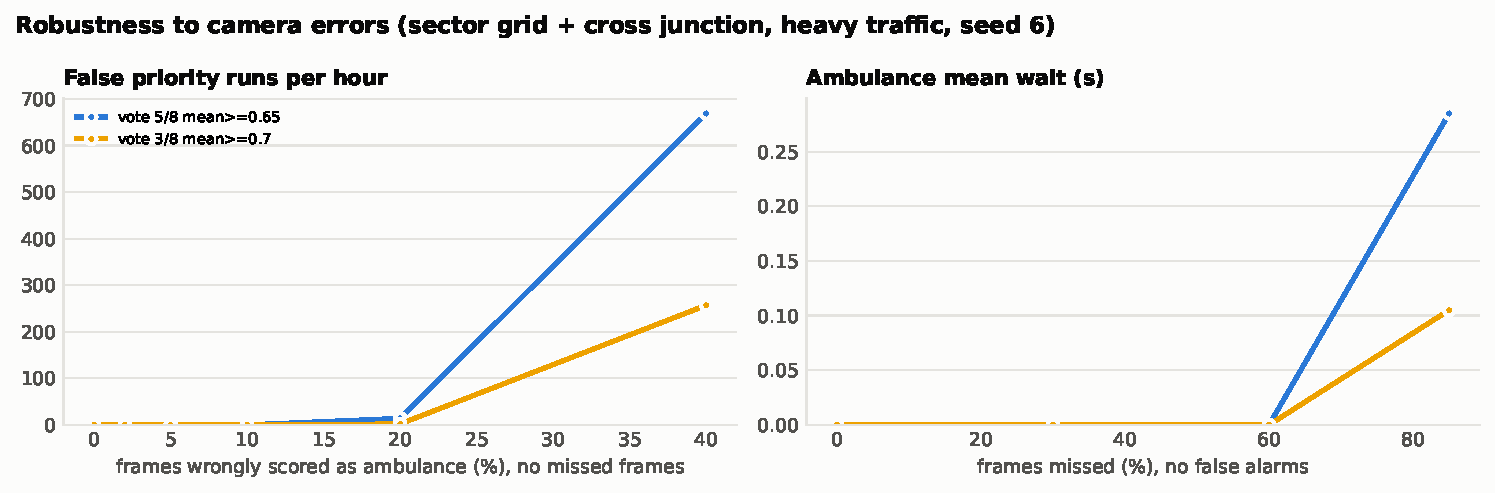
\includegraphics[width=\textwidth]{figures/fig_robustness.pdf}
\caption{False priority runs and ambulance wait as the virtual camera misses frames or scores ordinary
vehicles as ambulances, for the 5-of-8 vote and the live 3-of-8 vote (heavy demand, seed 6).}
\label{fig:it2-robust}
\end{figure}

The sweep was run for both votes (Figure~\ref{fig:it2-robust}). With up to 10\% of frames wrongly scored as
ambulance, neither produces any false priority. At 20\% the 5-of-8 vote (mean $\geq$ 0.65) produces 8--20 false
priority runs per hour and the live 3-of-8 vote (mean $\geq$ 0.70) only 0--4; at 40\% they produce 386--952
and 145--369. The live vote is therefore more tolerant of noisy frames, not less: its stricter mean-score
threshold matters more than the lower vote count. Missing even 85\% of frames barely matters (ambulance wait at
most 0.6\,s). The classifier's per-crop false-alarm rate is 0.9\% on the test split, well inside this margin.

\subsection{Ambulance classifier}
\label{sec:it2-classifier}
\paragraph{Dataset check.} \texttt{Projects/make\_split\_manifest.py} lists all 32\,593 crops with a SHA-1 and a
perceptual hash and looks for images shared between splits. The test split contains no exact copy of a training
image; 134 test crops (3.6\%) are near duplicates of a training crop, all with the same label. The check found
four validation crops labelled ambulance that were copies of training crops labelled other vehicle, and 35
duplicate files inside the training split; all 39 were removed. Removing the four mislabelled copies alone raised
the mid-report model's validation recall from 91.0\% to 91.8\%: all four had been counted as missed ambulances.

\paragraph{Retraining.} Three changes proposed in the mid-report were trained one at a time on the cleaned data and
compared on the validation split only (Table~\ref{tab:it2-cls-val}). Retraining with unchanged settings changes
little; doubling the ambulance crops gives the highest recall but more false alarms; a 128\,px input
(cls\_v5\_img128) is best on PR-AUC and F1 and was selected.

\paragraph{Test split.} Only the selected model and the mid-report model were then run on the held-out test split,
once (Table~\ref{tab:it2-cls-test}). cls\_v5\_img128 is better on every metric: 93.5\% recall at 96.5\% precision
and a 0.9\% false-alarm rate. Recall is lowest on the Pakistani ambulance crops (88.1\%, against 95.9\% on the
public dataset). A threshold chosen on the validation split for 95\% recall gives 95.7\% test recall for the
mid-report model, at 87.7\% precision.

\paragraph{Latency.} On an RTX 4050 laptop GPU the vehicle detector takes 27.7\,ms per 1280\,px frame and the
classifier 1.7\,ms per crop in a batch (Table~\ref{tab:it2-latency}): about 45\,ms per frame, or 22 frames per
second, with ten vehicles in view. Measured back to back, the 128\,px classifier costs the same as the 96\,px one.

\subsection{Tracking on real video}
\label{sec:it2-tracking}
With the new classifier and the old vote (5 of 8, mean $\geq$ 0.65) the pipeline confirmed 5 of the 7 labelled
ambulance passes. \texttt{Projects/tune\_tracking.py} records every track's score per frame once and replays the
vote offline; at the old setting the replay reproduces the pipeline's confirmations exactly on all 12 videos.
Of 360 settings (Table~\ref{tab:it2-tune}), the number of votes K decides the result: every setting with K = 3
and a mean score of 0.70--0.75 confirms all 7 passes with 6 false events, whatever the frame threshold, while
K = 4 or 5 confirm 5. The chosen setting keeps the frame threshold at 0.6 and uses K = 3, mean $\geq$ 0.70.

Table~\ref{tab:it2-tracking} gives the re-run pipeline on all 12 available clips (a thirteenth clip has no source
video): 7 of 7 passes confirmed, on average 0.94\,s after the labelled start, with 6 false confirmations: 3 in
test5, a clip checked to contain no ambulance (a look-alike vehicle), 2 in test12 1.4\,s before a labelled pass,
and 1 in test4. Because the same videos chose and scored the setting, this is optimistic. Choosing the setting on
11 videos and scoring the twelfth, for each video in turn, gives 7 of 7 passes and 11 false events. Seven passes
are far too few for a reliable recall estimate.

\subsection{Performance}
A controller tick takes about 1\,$\mu$s and a MARL decision about 24\,$\mu$s (p99 62\,$\mu$s), against a
100\,000\,$\mu$s tick period (Table~\ref{tab:it2-perf}). A one-hour SUMO run takes about 3\,s.

\section{Failure Analysis}
\begin{table}[htbp]
\centering
\small
\caption{Failure cases found in Iteration 2 and the planned response.}
\label{tab:it2-failures}
\resizebox{\textwidth}{!}{%
\begin{tabular}{lll}
\hline
Failure & Likely cause & Response \\
\hline
Short ambulance tracks missed with a 5-of-8 vote (test12) & too few confident frames before it leaves & resolved: K = 3, re-tuned \\
3 false confirmations in test5 (no ambulance) & ambulance-like vehicle not in training & add its crops as hard negatives \\
Early confirmations (test12, 1.4\,s before the label) & hand-labelled windows are approximate & label from the first visible frame \\
Recall 88\% on Pakistani ambulances (test) & few local ambulance crops in training & collect more local ambulance crops \\
Mislabelled duplicate crops (4 in validation) & copies made while sorting crops & resolved: split manifest + duplicate check \\
False priority at $\geq$20\% per-frame false alarms & vote too permissive for very noisy input & keep per-frame FP $\ll$ 20\%; live 3-of-8 vote is 4$\times$ more tolerant \\
Higher p95 wait than actuated under heavy demand & green length fixed at its start & resolved: extension + tail tuning (gap +0.3\,s, n.s.) \\
Green extension lengthened the longest wait (+6.6\,s) & others held up to the 40\,s cap & resolved: 30\,s cap, wait weight 0.3 \\
Corridor gives no measurable ambulance benefit & junctions 300\,m apart & off by default; just-in-time rule kept as an option \\
Fair recovery gives no benefit (harmful when frequent) & adaptive order already serves delayed approaches & off by default; re-order rule removes the harm \\
MARL better on car wait, worse on tail waits & heuristic tail tuning moved further & longer training, tail-weighted reward \\
\hline
\end{tabular}}
\end{table}

\section{Limitations}
All control results are from simulation; the SUMO cameras are virtual (exact ambulance positions with
simulated classifier scores), so the real camera pipeline and the SUMO evaluation share the controller and the
voting rule but not the video. The live vote (3 of 8) was tuned on the same 12 clips it is scored on, which
hold only 7 ambulance passes. The fair-recovery stress scenario is one synthetic demand pattern. Authentication
is off by default and must be enabled for any deployment.

\section{Iteration Outcome}
The exit criterion is met: the scripted scenario (\texttt{scripts/scripted\_scenario.py}) sends one ambulance,
then two simultaneous ambulances; each is confirmed by detection, receives a protected green, and is followed
by recovery greens, and the whole sequence is recorded in the event log. All 45 automated tests pass. The classifier
was evaluated on the held-out test split and replaced by a better retrained model, all available videos were
processed, and the improvements the first evaluation pointed to were implemented and evaluated on the held-out
seeds: green extension and tail tuning (which closed the heavy-demand gap to actuated control), an approach-level
fairness measure, a re-order-only recovery rule and a recovery stress test, a just-in-time corridor, a retrained
MARL policy and the camera-error sweep for the live vote. Fair recovery and the corridor did not help and are off
by default. The main open items for FYP-2 are reducing the delay of the vehicles an ambulance holds (the cost of
priority that remains), MARL training that also wins on tail waits, more labelled real video, and hard negatives
for ambulance look-alikes.
